\documentclass[12pt]{article}
\usepackage[margin=2.5cm]{geometry}
\usepackage{amsmath}
\usepackage{amssymb}
\usepackage{mathtools}  
\usepackage{diffcoeff}  
\usepackage{siunitx}
\usepackage[table,xcdraw]{xcolor}
\usepackage{amsfonts}
\usepackage{subfiles}
\usepackage{hyperref}
\usepackage{newtxtext, newtxmath}
\usepackage{enumitem}
\usepackage{titling}
\usepackage{listings}
\usepackage{float}
\usepackage{hyperref}
\setlength{\droptitle}{-6em}
\usepackage{placeins}
\usepackage{graphicx}
\usepackage{subcaption}
\usepackage[utf8]{inputenc}
\usepackage{fancyhdr}
\usepackage{color}
\usepackage{xspace}
\usepackage{pifont}

%%% This is about changing the headers and footers (i.e. Top and bottom of the page)
\pagestyle{fancy}% use fancyheaders with the bar on the top
\fancyhf{} % Clear the normal style
\fancyhead[L]{\bfseries\leftmark} %this places the section number and name in the top left
\fancyhead[R]{\bfseries\thepage}% this places the pagenumber in the top right
%%%% Add the bibliography with some settings:
% package:
% \usepackage[square, comma, numbers, sort&compress ]{natbib}
\usepackage[style=authoryear,citestyle=authoryear,maxcitenames=2,maxbibnames=20,uniquename=false,uniquelist=false,eprint=false]{biblatex}
\addbibresource{bibbestand.bib}

\renewbibmacro*{doi+eprint+url}{%   
  \iftoggle{bbx:url}     
    {\iffieldundef{doi}{\usebibmacro{url+urldate}}{}}     
    {}%   
  \newunit\newblock   
  \iftoggle{bbx:eprint}     
    {\usebibmacro{eprint}}     
    {}%   
  \newunit\newblock  
  \iftoggle{bbx:doi}     
    {\printfield{doi}}     
    {}}

%%%%% frontmatter/mainmatter/backmatter:
\newcommand\frontmatter{%
    \cleardoublepage
    \pagenumbering{roman}} %small Roman numbers

\newcommand\mainmatter{%
    \cleardoublepage
    \pagenumbering{arabic}} %normal numbers

\newcommand\backmatter{%
    \cleardoublepage %% double page style
    %\clearpage %% single page style
    \pagenumbering{Roman}} %capital Roman numbers


\begin{document}
\newgeometry{margin=1.5cm} %% Special margins on the titlepage. It is also possible to set each margin separately; see package Geometry.
%%% Titelpagina in een apart bestand

\begin{titlepage} %%% This is your titlepage. Everything should match the conditions as they are right now for a physics thesis; hopefully the conditions won't change soon. In order to change this page into your very own title page, replace the noted parts with your own (like 'Your title').
	\noindent
    \begin{minipage}{0.4\textwidth}
        
\includegraphics[height=0.2\textheight]{UU_logo_2021_NL_RGB.png}
    \end{minipage}\hfill
    \begin{minipage}{0.4\textwidth}
        
\includegraphics[height=0.1\textheight]{logoIMAU_hd.png} 
    \end{minipage}
    \par\vspace{0.5cm}
    \begin{center}
    {\huge\bfseries Emulating SAI Scenarios in CESM2 and the Effects on the Southern Hemisphere Large-Scale Atmospheric Circulation\par} %% ENTER TITLE HERE
    \end{center}
	\vspace{1cm}
    {\scshape\Large Master Thesis\par}
	\vspace{0.5cm} % You change this to set the distance 'Bachelor Thesis' to 'Your name', and all the other vspaces to set the heights of everything.
	{\Large\itshape Simone Lingbeek\par}
    {\large Climate Physics\par}
    \vspace{6cm}
    % \centering
    % \fbox{ %% fbox puts a black border around your picture
    % \includegraphics[height=0.35\textheight]{Clipboard01} %% If you use a picture, place it here. If you don't, delete this, from '\centering' to '\par'.
    % %% change the height ration until it fits.
    % } %% the fbox ends here
    % \vspace{0.5cm}
    % \par
    \raggedleft
	{\Large\itshape Supervisors}:\par\vspace{0.25cm}
	{\large Dr. Claudia Wieners\par} %% first supervisor
    Institute for Marine and Atmospheric research Utrecht (IMAU)\par %% their institute
    \vspace{0.25cm}
    {\large Dr. Michiel Baatsen\par} %%second supervisor
    Institute for Marine and Atmospheric research Utrecht (IMAU)\par %% their institute
    \vspace{0.5cm}
	{\Large\itshape Daily supervisor}:\par\vspace{0.25cm}
    {\large Jasper de Jong\par} %%daily supervisor
    Institute for Marine and Atmospheric research Utrecht (IMAU) %% their institute
    %% copy/paste from \vspace{0.25cm} to here for more supervisors.

	\vfill
	{\large July 2024 \par}%%% The date. Replace \today with the necessary date if your necessary date isn't today.
    
\end{titlepage}    

\restoregeometry %%% Restores the margins for the rest of the document.


\tableofcontents
\newpage

\section{Introduction}
\subsection{Climate change and geoengineering}
In the effort of limiting the effects global climate change, eliminating fossil fuels is the most important step to take. Regrettably, the complete elimination of fossil fuels in time to prevent the most disastrous effects of climate change and limit global warming to even 2°C is becoming increasingly unlikely. Even with all currently committed climate action goals, projections show the earth warming significantly above the 1.5°C and 2°C targets from the Paris Agreement \parencite{NDCsynth}. With this outlook, methods to temporarily lower the earth's global temperature are looked at to buy the global community time to lower atmospheric greenhouse gases. One such method is solar radiation management with stratospheric aerosol injections (SAI). 

Geoengineering can be seen as a toolbox of methods that change the earth's climate system to achieve a desired effect. Limiting global mean surface temperature (GMST) increase is the primary goal of geoengineering. The methods of geoengineering can be divided into two basic categories, Carbon Dioxide Removal (CDR) and Solar Radiation Management (SRM) \parencite{shepherd2009}. CDR focuses on lowering the amount of greenhouse gases in the atmosphere, by capturing CO$_2$ directly or enhancing and facilitating natural processes to speed up the extraction of CO$_2$ from the atmosphere or oceans. SRM on the other hand focuses on altering the earth's radiation budget. This can be done by increasing the amount of long wave radiation the earth emits into space, for instance with cirrus cloud thinning, but the most widely discussed approach is increasing how much short wave radiation from the sun is reflected back into space, i.e. increasing the planetary albedo. This is done for instance by making deserts more reflective or making clouds brighter like through marine cloud brightening \parencite{reflecting}. 

\subsection{Geoengineering in the Form of Stratospheric Aerosol Injections}
This thesis considers SRM in the form of stratospheric aerosol injections (SAI). Through injection of sulphate aerosols or their precursors at specific points in the stratosphere the earth's radiation budget is changed. At this high altitude the aerosols reflect short wave radiation, lowering the amount of sunlight reaching the earth's surface and subsequently GMST is lowered. It has been argued that SAI is one of the most feasible options for SRM \parencite{lenton2009,shepherd2009}.

A direct result of SAI is the absorption of long wave radiation emitted by the earth by the aerosols, resulting in warming in the stratosphere \parencite{Ammann2010}. This impacts the global atmospheric circulation patterns and precipitation patterns. It is also important to keep in mind that the effects other than warming caused by increased greenhouse gases are still present in the earth system, for instance ocean acidification will continue if CO$_2$ concentrations continue to rise. The introduction of sulphate aerosols has unintended consequences too, including in delayed repair of the ozone hole and an increase in acid deposition, and interference with cloud formation. 

Eventhough complete understanding of the physical consequences of SAI is not within reach as of now, the physical feasibility in regards to limiting global warming is rather certain. Practically, the succesful deployment of SAI is only possible if the global community can reach consensus on its employment and can ensure no party deploys SAI undemocratically and to the detriment of others. Even then, long-term political and economical stability are crucial, as an abrupt halt would lead to rapid warming \parencite{robock2009}. 

The employment of SAI is not as straight-forward as appears at first glance, and before any decisions can be made about SRM, with SAI or through other means, more research is needed. The National Academy of Sciences made extensive recommendations for solar geoengineering research \parencite{reflecting}, including research into the impacts on atmospheric processes, the climate response, desigining a monitoring system, how to govern solar geoengineering activities and ethical considerations for current and future generations. 

\subsection{General Structure}
In this thesis we investigate the climate response to SAI, more specifically the atmospheric dynamics of the Southern Hemisphere. We will use the results from a previous study on SAI conducted with an earth system model with an extensive atmospheric component and comprehensive atmospheric chemistry to build an emulator with a model with a smaller atmospheric component that incorporates no atmospheric chemistry. We do this primarily to save on computation time. We will validate this experiment in Part I, and use it to assess the impact of SAI on the Southern Hemisphere atmospheric circulation in Part II. We will focus on changes in the large scale components of the atmospheric circulation. 

The southern hemisphere is of particular interest because of the Antarctic Ice Sheet that is home to a number of tipping points. The triggering of these tipping points can potentially lead to disastrous levels of sea level rise and once these tipping points are reached, there is no way to reverse the effects. Understanding the dynamics of the Southern Hemisphere and the response to SAI is crucial to accurately predict the future evolution of these tipping points and if triggering them can be avoided with the help of SAI. 

\newpage
\section{Introduction Part I}
\subsection{Previous Research on SAI in Earth System Models}
Large scale studies on SRM started with the Geoengineering Model Intercomparison Project (GeoMIP) \parencite{geomip2011}. Experiments reduced the incoming solar radiation either directly or through injection of SO$_2$ in the stratosphere at one point on the equator, which was then distributed in the atmosphere very quickly by the zonal circulation and on larger time scales the meridional circulation.

It was found that injection of aerosols at just the equator, and uniform solar radiation reduction lead to over-cooling of the tropics and under-cooling of the poles. \textcite{kravitz2016} proposed a different approach, where climate targets were considered the main goal and how to reach those goals through SAI was viewed as a design problem. One set of targets proposed was the global mean surface temperature ($T_0$), the interhemispheric temperature gradient ($T_1$) and the pole-to-equator temperature gradient ($T_2$). The proposed SAI strategy included four injection points, two on each hemisphere, and a feedback algorithm that adjusts the injection rate at those points to achieve the temperature goals. This method was applied by \textcite{kravitz2017} and \textcite{macmartin2017}, and then in the Geoengineering Large Ensemble (GLENS) project \parencite{tilmes2018}. 

\subsection{The GLENS Project and Subsequent CESM2 Simulations}
The GLENS project is a 20-member ensemble of gradual SAI simulations. From 2020 onwards SO$_2$ is injected at four injection points at $\pm$ 15°N and $\pm$ 30°N about 5 km above the tropopause. A feedback-control algorithm is used to adjust the injection amounts at each point individually based on the departure of the $T_{0,1,2}$ temperatures defined by \textcite{kravitz2016} from 2020 levels.

The GLENS project was performed using the Community Earth System Model version 1 (CESM1) \parencite{hurrell2013}, with the Whole Atmosphere Community Climate Model (WACCM) as its atmosphere component. This model uses a 0.9° latitude $\times$ 1.25° longitude rectangular grid with 70 vertical layers that reach up to 140 km, or about 10$^{-6}$ hPa. It includes comprehensive atmospheric chemistry for the middle atmosphere, incorporating ozone chemistry and chemistry relating to stratospheric sulfate formation. A simpler chemistry scheme is used for the troposphere. Aerosol chemistry is coupled to WACCM through the three-mode version of the Modal Aerosol Module (MAM3).

After the GLENS project the method using four injection points and a feedback algorithm was further explored using the more recent Community Earth System Model version 2, also using a newer version of the WACCM, now version 6 (CESM2(WACCM6)) \parencite{tilmes2020}. WACCM6 has the same horizontal and vertical resolution, but now includes comprehensive chemistry from the troposphere up to the lower thermosphere. The MAM4 modal aerosol scheme is used for the troposphere and stratosphere. We will refer to this model as `WACCM'.

Because WACCM is comprehensive in both vertical resolution and atmospheric chemistry, it is well-suited to simulate SAI scenarios. However, due to this it is also a very cumbersome model, requiring more computing time and resources compared to less comprehensive models. This limits its use in ensemble studies and studies considering a large range of scenarios. Computational cost also limits its use for simulations with a longer timeseries at higher resolution, required to study smaller scale phenomena like tropical cyclones. 

\subsection{Building an Emulator for SAI with CESM2(CAM6)}
Reducing the amount of computing resources needed for an experiment can be done by using a smaller, less comprehensive model and using previous results from WACCM as external forcing to the model, essentially building an emulator. \textcite{pfluger2024} introduce a method for building such an emulator of WACCM to model SAI. They use the same CESM2 model configuration is used as in \textcite{tilmes2020}, but the Community Atmosphere Model version 6 (CAM6) is used for the atmosphere component \parencite{danabasoglu2020}. This model has only 32 vertical levels and no atmospheric chemistry. We will refer to this model as `CAM'. The aerosol field established in the WACCM simulation is used as an external forcing. To maintain 2020 levels of GMST, the necessary globally averaged aerosol optical depth (AOD) field is found though the same feedforward-feedback algorithm. All other forcing fields are then scaled accordingly. In contrast to the WACCM simulations, the temperature gradients $T_1$ and $T_2$ are not adjusted for. 

The WACCM SAI experiment is well-suited to build an emulator for, as the employment of SAI is used as a means to reach a climatic goal. It prescribes an aerosol burden in response to model behaviour, in stead of gauging the model response to a certain aerosol burden. This removes the amount of SO$_2$ injected into the stratosphere from the experiment design and allows for translation of the aerosol distribution to another model that might respond differently to the introduction of aerosols.

\subsection{Scenarios Part I}
There are two simulations performed with CAM and WACCM. The first simulation follows the historical spin-up and is continued by the SSP5-8.5 scenario \parencite{RIAHI2007887}. The second simulation branches from the first simulation in 2020 and from then on introduces SAI to stabilise temperatures using the SSP5-8.5 scenario as background. Here we will refer to it as the gradual SAI scenario. A schematic view of the GMST response in each scenario is shown in Figure \ref{fig:schematic_scens_pt1}.

\begin{figure}[H]
    \centering
    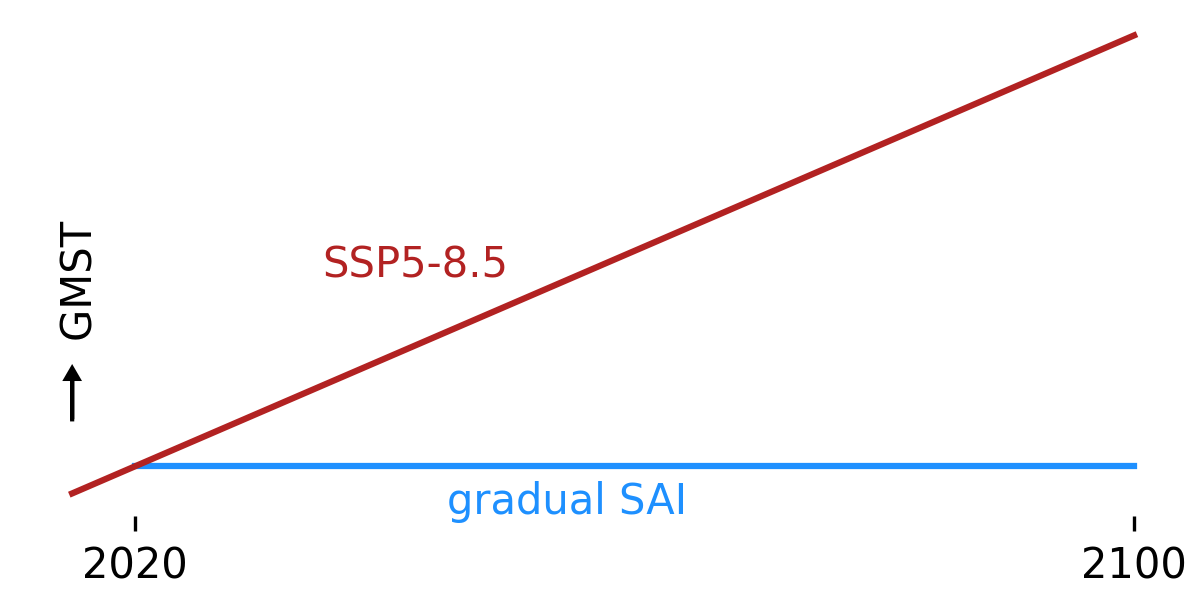
\includegraphics[width=0.6\linewidth]{images/schematic_scens_pt1.png}
    \caption{Schematic of the global mean surface temperature in the two scenarios used in Part I, the SSP5-8.5 and gradual SAI scenarios.}    
    \label{fig:schematic_scens_pt1}
\end{figure}


\newpage
\subsection{Research Questions Part I}
The fist part of this thesis is the validation of this method and model in its use as an emulator, simulating SAI scenarios based on the WACCM results. Two experiments, a high-warming scenario and a gradual SAI scenario, are used to assess the impact of SAI in each model (CAM and WACCM). We calculate the three temperature targets for all models and we will look at the model results for 2-meter temperature for additional insight into the performance of CAM in regards to regulating surface temperatures. We discuss both annual and seasonal patterns. Additionally, we discuss precipitation patterns.

The most important difference in dynamics between the two models lies in the inclusion of ozone chemistry and thus the interaction of stratospheric aerosols and ozone. It is known that sulphate aerosols in the stratosphere accelerate chemical ozone loss through halogen activation and strengthening of the polar vortex \parencite{bednarz2023ozone}. CAM does not include this process, and assessing whether the dynamical response to SAI is comparable to WACCM is thus important. To this end we assess any differences in the vertical profile between the two models, we compare the zonally averaged potential temperature and zonal winds. 

We formulate the following research questions for Part I:
\newline

\noindent \textit{When applying the stratospheric aerosol emulator to a gradual SAI scenario in CESM2(CAM6), are we able to reproduce from \textcite{tilmes2020}
    \begin{enumerate}[label=\roman*]
        \item the temperature targets $T_0$, $T_1$ and $T_2$?
        \item the spatial and seasonal variations of temperature, precipitation and general aspects of the atmospheric circulation?
    \end{enumerate}
}

\subsection{Results SAI in WACCM}
The experiments performed with WACCM \parencite{tilmes2020} showed that surface temperatures were generally controlled with SAI. Under SAI the tropics warmed slightly, the mid-latitudes cooled slightly and the poles warmed slightly as well. Zonal mean precipitation showed an increase in the tropics and a decrease or no significant change everywhere else. An apparent warming hole over the Northern Atlantic was observed in all simulations and was likely related to observed changes in the Atlantic Meridional Overturning Circulation. No changes in seasonal patterns were discussed, nor were changes in potential temperature and atmospheric circulation. 


\newpage
\section{Introduction Part II}
\subsection{Rapid Cooling with SAI as an Emeregency Intervention}
As sufficient climate policies to prevent global warming of 1.5°C or even 2°C \parencite{NDCsynth}, it is unlikely the global community will implement a proactive gradual SAI scenario in time as well. Employing SAI much later on after prolonged heating of the climate system is a realistic, more reactive, scenario. The earth could be cooled very rapidly, allowing the end-of-century GMST goals to be reached after the climate system has endured an even longer period of warming than it has to date. The effects of such an intervention are largely uncertain. While it is rather certain that SAI could lower GMST, it is not certain what effects of previous warming can be reversed, if at all. The SAI 2080 scenario introduced in \textcite{pfluger2024} is such a scenario, SAI is employed from 2080 onwards to achieve rapid cooling to 2020 levels. 

\subsection{Scenarios Part II}
For the second part of this thesis we consider the two CAM simulations from Part I, the SSP5-8.5 and the gradual SAI simulations, and the SAI 2080 scenario from \textcite{pfluger2024}. We will refer to this simulation as the rapid cooling SAI simulation. The rapid cooling simulation is branched from the SSP5-8.5 simulation in 2080, SAI is then deployed to restore $T_0$ to 2020 levels. The control algorithm is adjusted up to the first six years to prevent extremely high aerosol concentrations that would result in too rapid cooling. A schematic view of the GMST response for this scenario is shown in Figure \ref{fig:schematic_scens}.

\begin{figure}[H]
    \centering
    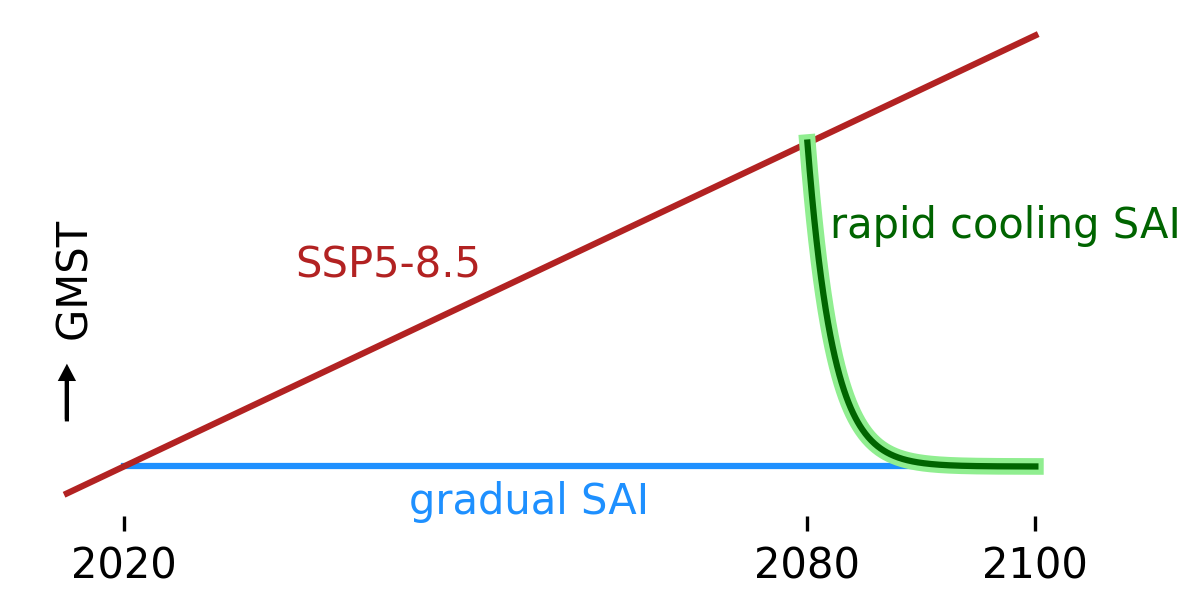
\includegraphics[width=0.65\linewidth]{images/schematic_scens.png}
    \caption{Schematic of the global mean surface temperature in the two scenarios used in Part I, the SSP5-8.5, the gradual SAI and the rapid cooling SAI scenarios.}  
    \label{fig:schematic_scens}  
\end{figure}


\subsection{The Southern Hemisphere Atmopshere}
The atmosphere is home to a number of large scale circulation phenomena. Though the two hemispheres are symmetrical in the occurence of these phenomena, the exact location, frequency of occurence and other behaviour of these phenomena differs between the two hemispheres. The Southern Hemisphere circulation is generally more stable than its counterpart in the Northern Hemisphere. In this thesis we focus on three so-called jets, large scale circulation phenomena that persist throughout the year or in a specific season.
We discuss the subtropical jet and the the eddy-driven jet in the lower stratosphere (up to 50 hPa), and the polar night jet in the upper stratosphere (above 50 hPa).


\subsubsection{The Subtropical Jet}
The subtropical jet (STJ) forms at the convergence of the upper branches of the Hadley and Ferrel cells in the lower stratosphere, with a maximum around 200 hPa, see Figure \ref{fig:jetcrosssection} (the Southern Hemisphere is analogous to the Northern Hemisphere). Influenced by the Coriolis force westerly winds form here, the magnitude of which is determined by the temperature gradient below the convergence zone \parencite{zolotov2018variability}. The STJ occurs year-round but is strongest in winter, in tandem with the stronger winter Hadley cell, where it is located around 30°S.

In the past decades, the southern hemisphere STJ has been observed to shift poleward and slightly decrease in wind speed, though not significant \parencite{zolotov2018variability}. The STJ was also observed to be increasingly wavy \parencite{martin2023}. Under high global warming the STJ is projected to shift further poleward and increase in strength \parencite{chenoli2017historical}. 

Simulations with SAI at singular injection points showed a small but significant decrease in the strength of the STJ \parencite{richter2017}. From historical simulations it has been argued as well that anthropogenic aerosols contribute to deceleration \parencite{wang2020}.

\begin{figure}[t]
    \centering
    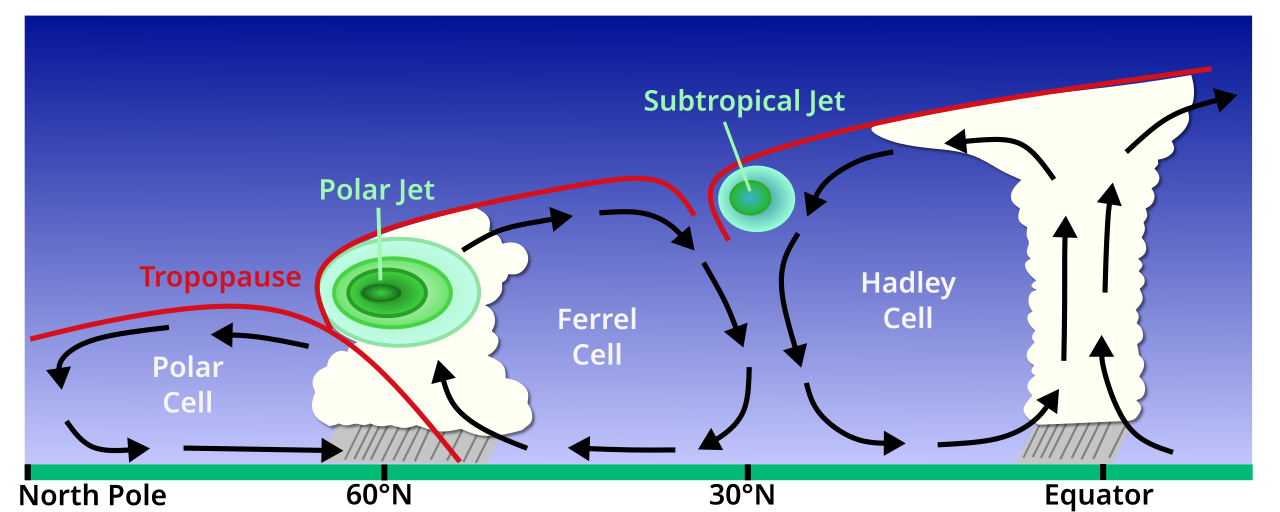
\includegraphics[width=0.8\linewidth]{images/Jetcrosssection.png}
    \caption{Cross section of the Northern Hemisphere atmospheric ciruclation, with the suptropical jet and polar jet (or eddy-driven jet) in relation to the circulation cells. Image by: Original: National Weather Service, JetStream Vector: Sleske - Own work based on: Jetcrosssection.jpg, CC BY-SA 4.0, \href{https://commons.wikimedia.org/w/index.php?curid=75169357}{https://commons.wikimedia.org/w/index.php?curid=75169357}}  
    \label{fig:jetcrosssection}  
\end{figure}


\subsubsection{The Eddy-driven Jet}
At the divergence of the upper branches of the Ferrel and Polar cells another jet forms, the polar jet in Figure \ref{fig:jetcrosssection}. This jet is at a lower altitude and stronger than the STJ. However, it is also much wavier than the STJ \parencite{martin2023}. Because of this, and to avoid confusion with the polar night jet, we will refer to this jet as the eddy-driven jet (EDJ). 

The EDJ has been observed to become increasingly wavy in the past decades, also shifting poleward, even more strongly than the STJ, but no significant trend in the wind speed was observed \parencite{martin2023}. Under high global warming the EDJ is projected to shift further poleward \parencite{Curtis_2020}.

It is not certain how the EDJ will respond under SAI, though it has been shown that the EDJ is influenced by the strength of the polar night jet in the upper stratosphere, where a strengthened jet leads to a poleward shift of the EDJ \parencite{kidston2015stratospheric}. Any changes in the polar night jet due to SAI are thus likely to cause changes in the EDJ as well.

\subsubsection{The Polar Night Jet}
The polar night jet (PNJ) forms in the upper stratosphere during winter in response to the large equator-to-pole meridional temperature gradient. The pole becomes encircled with a belt of strong westerly winds in the upper parts of the stratosphere, above $\approx$50 hPa at around 60°S \parencite{lee2021}. 

With high warming the PNJ is projected to increase in strength, most notably in late SH spring, effectively delaying the ultimate breakdown of the PNJ \parencite{ceppi2019}.

The warming in the lower stratosphere due to SAI leads to an increase of the equator-to-pole meridional temperature gradient, causing increasing zonal winds via the thermal wind balance. This effect is strongest in the late winter/early spring \parencite{bednarz2023injection,bednarz2023ozone}.

When disturbances near the surface propagate to the stratosphere, the PNJ can suddenly weaken, leading to a sudden increase in temperatures of the polar stratosphere and sometimes a complete breakdown of the jet. These events are called sudden stratospheric warming events (SSWs) and occur very rarely in the Southern Hemisphere in the current climate. Their frequency is projected to strongly decrease with increasing global warming \parencite{jucker2021}. 


\subsection{Antarctica and the Southern Hemisphere Atmosphere}
The high-latitude Southern Hemisphere is of particular interest in the context of climate change and the prevention of it. The Antarctic Ice Sheet (AIS) could contribute greatly to global sea level rise if it were to become unstable under global warming. Observed instabilities of the West-Antarctic Ice Sheet (WAIS) alone could contribute to significant sea level rise \parencite{IPCC_2021_WGI_Ch_9}. 

Large scale atmospheric dynamical changes affect the Antarctic ice sheet, changes in temperature, precipitation and wind fields alter the surface mass balance of the ice sheet. More distantly dynamical changes affect the ice sheet through changes in the ocean, mainly in the rate and location of overturning circulations. A warmer ocean together with a warmer atmosphere can lead to the loss of ice shelves \parencite{WANG2023} and their disappearance has been observed to increase the flow of glaciers feeding into the ocean \parencite{scambos2004}, contributing to mass loss of the AIS. 

The Southern Hemisphere high stratosphere has low variability in the current climate, but any changes could have far-reaching effects on the surface climate. It has been observed that SH stratospheric polar vortex weakekening contributes to climate anomalies in Australia and New Zealand, southeast Africa and southern South America. Additionally, the wind stress over the ocean around Antarctica is weakened and the Ross and Amundsen seas experience warmer climate \parencite{domeisen2020}. There is thus a clear interaction between the atmospheric dynamics and local climate in the Southern Hemisphere. 

The effect of SAI on the Antarctic ice sheet has been studied by \textcite{mccusker2015}, who found that a rapid introduction of sulphate aerosols in the stratosphere could not prevent the collapse of the WAIS. \textcite{sutter2023} found similar results. However, both studies use very simple aerosol schemes, that for instance only inject aerosols in the tropics. These types of schemes are known to lead to over-cooling of the tropics and under-cooling of the poles. As stated before, the studies using a feedback-control algorithm to maintain the $T_{0,1,2}$ temperature targets were laregely successful in this regard. 


\subsection{Research Questions Part II}
In the second part of this thesis the effect of SAI on the high-latitude Southern Hemisphere atmospheric dynamics is investigated, both in the gradual and rapid cooling scenarios. The focus here lies on large scale circulation patterns, as they largely dictate local climate in the Southern Hemisphere. 

We formulate the following research quesitons for Part II:
\newline

\noindent \textit{What are the impacts of the gradual SAI scenario on the Southern Hemisphere
    \begin{enumerate}[label=\roman*]
        \item subtropical and polar jets in the lower stratosphere?
        \item polar night jet and sudden stratospheric warming events in the upper stratosphere?
    \end{enumerate}
How do the results for i and ii change under the rapid cooling SAI scenario?
}
\newpage

\part{Model Validation}

\section{Methods Part I}
\subsection{Temperature Targets}\label{temptargets}
The WACCM simulations use the feedback algorithm to maintain three temperature targets in their SAI scenario. These temperature targets are defined in \textcite{kravitz2016} as the projection of $T(\psi)$ onto the first three components of the Legendre polynomial expansion of $\sin(\psi)$,

\begin{equation}\label{eq:Tpsi}
    \begin{split}
        T_0 &= \frac{1}{2} \int\displaylimits_{-\pi/2}^{\pi/2} T(\psi) \cos(\psi) \mathop{d\psi},\\
        T_1 &= \frac{1}{2} \int\displaylimits_{-\pi/2}^{\pi/2} T(\psi) \sin(\psi) \cos(\psi) \mathop{d\psi},\\
        T_2 &= \frac{1}{2} \int\displaylimits_{-\pi/2}^{\pi/2} T(\psi) \frac{1}{2}(2\sin^2(\psi) -1) \cos(\psi) \mathop{d\psi},
    \end{split}
\end{equation}

\noindent where $\psi$ is latitude, $T(\psi)$ is the zonal-mean temperature for each latitude.

The $T_0$ temperature target translates to global mean surface temperature (GMST), the $T_1$ is interpreted as the inter-hemispheric temperature gradient and $T_2$ is interpreted as the equator-to-pole temperature gradient. From the model output these temperature targets can be evaluated using Eq. \ref{eq:Tpsi}. 


\subsection{Using the CESM2(CAM6) Emulator for SAI simulations}\label{emulator_pt1}
The emulator for SAI simulations is introduced in \textcite{pfluger2024}, it implements SAI via prescribed aerosol fields, as opposed to sulphate injections that result in aerosol fields through model physics. As per \textcite{pfluger2024}, the protocol works as follows:
\begin{itemize}
    \item Every year, observe the deviation of GMST from the target.
    \item Based on past GMST deviations, infer the level of SAI - expressed in terms of global mean aerosol optical depth (AOD) - which is necessary to achieve the desired target.
    \item Use the AOD to scale all SAI-related aerosol fields appropriately.
    \item Feed the scaled fields into CAM6.
\end{itemize}

The first two steps are implemented via the feedforward-feedback control algorithm as established in \textcite{kravitz2017}. The control algorithm stabilises only GMST, not inter-hemispheric and equator-to-pole temperature gradients from section \ref{temptargets}.

The prescribed aerosol fields are the averaged aerosol fields from the WACCM simulation, this simulation is called the \textit{Geo SSP5-8.5 1.5 scenario} in \textcite{tilmes2020}. The fields are normalised, averaged and fit, to then arrive at an amplitude for each aersol component.

\textcolor{teal}{Stukje over aerosolveld hoe het eruit ziet + jaarlijkse totale massa figuren}


\subsection{Definition of Scenarios and Time Periods for Part I}
There are two simulations performed with each CESM2 configuration. The first simulation follows the historical spin-up and is continued by the SSP5-8.5 scenario. The second simulation branches from the first simulation in 2020 and from then on introduces SAI to stabilise temperatures using the SSP5-8.5 scenario as background. Here we will refer to it as the gradual SAI scenario. 

Throughout this first part, three time periods are selected to visualise and interpret the results from the simulations. For each period the 20-year mean is taken, unless specified otherwise. These periods are defined as follows:

\begin{itemize}
    \item \textbf{Reference} The period 2016-2035 of the SSP5-8.5 simulation.
    \item \textbf{Control} The period 2080-2099 of the SSP5-8.5 simulation.
    \item \textbf{SAI 2020} The period 2080-2099 of the gradual SAI simulation.
\end{itemize} %tabel van maken


\subsection{Vertical Interpolation}
The atmospheric vertical levels of CESM are defined at hybrid pressure coordinates. However, for ease of computation and visualisation, conversion to pressure coordinates is preferred. The hybrid pressure coordinates are converted to pressure coordinates for each timestep at each gridpoint. Then a logarithmic interpolation scheme is used to project the model output onto uniform constant pressure coordinates. For a variable $f$ at pressure coordinate $p$ the scheme takes the form

\begin{equation}
    f = \frac{f_1 - f_0}{\ln\frac{p_1}{p_0}} \cdot \ln \frac{p}{p_1} + f_0.
\end{equation}

For CAM the model output is converted to 34 pressure levels ranging from 3.5 to 993 hPa. We add two levels in the upper stratosphere, compared to the model output, for ease of analysis of patterns. For WACCM the SSP5-8.5 model output was pubplished in pressure levels, 19 pressure levels ranging from 1 to 1000 hPa. The WACCM gradual SAI scenario model output is converted to those same 19 pressure levels to enable direct comparison.

No interpolation is needed of the horizontal grids as these are identical in all models. 


\subsection{Potential Temperature}
With the vertical coordinate converted to pressure coordinates, the potential temperature $\theta$ is calculated through
\begin{equation}
    \theta = T\left( \frac{p_{ref}}{p} \right)^\kappa, 
\end{equation}
where $T$ is the air temperature, $p_{ref} = 1000$ hPa is the reference pressure, $p$ is the pressure. $\kappa$ is the ratio $\frac{c_p - c_v}{c_p}$, with $c_p = 1004$ J kg$^{-1}$ K$^{-1}$ the specific heat of an ideal gas at constant pressure and $c_v = 717$ J kg$^{-1}$ K$^{-1}$ that at constant volume. 

\newpage

\section{Results Part I}
This section contains the results of the comparison between the CAM and WACCM simulations. 

\subsection{Temperature Targets}
The deviations from the temperature targets in Eq. \ref{eq:Tpsi} were calculated from 2-meter temperature for all simulations. The results are shown in Figure \ref{fig:Tgrad1}. The results from the SSP5-8.5 simulations with CAM and WACCM are near identical for $T_0$, showing comparable variability and arriving at virtually the same final GMST. The results from the graudal SAI simulations are also comparable, both simulations succeeding in maintaining 2020 GMST levels with comparable variability. 

Deviations from $T_1$ and $T_2$ are again comparable in CAM and WACCM. The SSP5-8.5 simulation in CAM arrives at a deviation from $T_1$ about 25\% lower than in WACCM, but given the large variability present in both models this is not significant. The gradual SAI simulation in CAM is again comparable to WACCM, maintaining $T_1$ and $T_2$ with similar variability. 

\begin{figure}[H]
	\centering
	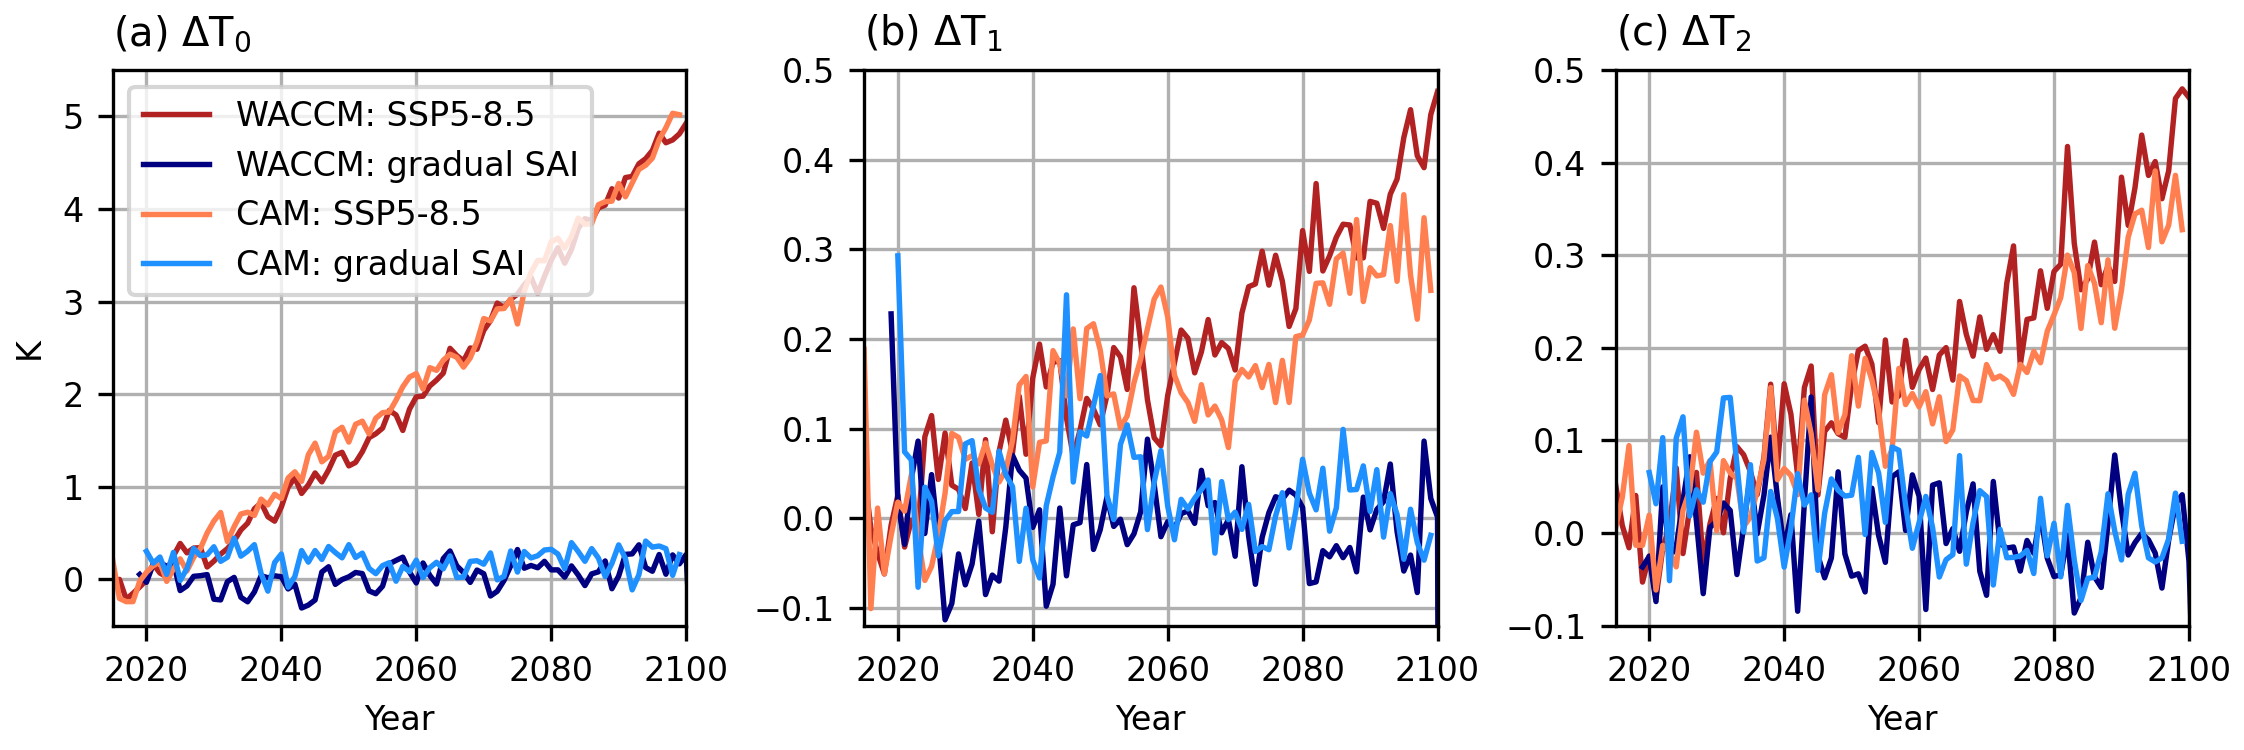
\includegraphics[width=0.95\linewidth]{images/Tgrad_v.png}
	\caption{Deviations from temperature targets $T_0$, $T_1$, $T_2$ as compared to 2016-2025 mean, for the SSP5-8.5 and gradual SAI scenarios in CAM and WACCM.}
	\label{fig:Tgrad1}
\end{figure}


\subsection{2-meter Temperature and Precipitation in CAM}
Figure \ref{fig:CAM_scens} shows the Reference 2-meter temperature and precipitation, their anomalies for Control compared to the Reference and their anomalies for SAI 2020 compared to Control. In Figure \ref{fig:CAM_scens}(b) the Control period shows expected warming patterns, with the land area warming more than the sea and the poles warming more relatively due to polar amplification. Higher warming off the coast of Antarctica and in the Arctic Ocean indicates a retreat of sea-ice at both poles. The anomalous warming over the eastern Pacific ocean resembles the spatial sea surface temperature pattern of El Ni\~no. The slight cooling over the northern Atlantic ocean resembles a North Atlantic warming hole, generally attributed to changes in ocean heat transport and weakening of the Atlantic meridional overturning circulation (AMOC) but also atmospheric circulation changes due to anthropogenic forcing \parencite{menary2018anatomy,he2022}. 

The SAI 2020 anomaly compared to the Control, shown in Figure \ref{fig:CAM_scens}(c), shows that SAI is able to compensate for most of the warming in Control. The land area is cooled more than the sea, as are the poles. Sea-ice retreat is largely prevented in both the Arctic and the Antarctic. The anomalous warming over the eastern Pacific ocean is not prevented, as well as the North Atlantic warming hole. 

The precipitation anomaly in Control, shown in Figure \ref{fig:CAM_scens}(e), shows a general increase in precipitation. Most significant drying can be attributed to a shift in the intertropical convergence zone (ITCZ), with a southward shift over the Atlantic and eastern Pacific Ocean, expected patterns under increased anthropogenic forcing \parencite{mamalakis2021zonally}. The shift over the eastern Pacific Ocean is possibly related to the El Ni\~no pattern observed in Fig. \ref{fig:CAM_scens}(b). No significant shift or other change in ITCZ is observed over the Indian and western Pacific Ocean.

In Figure \ref{fig:CAM_scens}(f) the precipitation anomaly of SAI 2020 compared to Control shows opposite trends, apparently preventing most increase in precipitation. The southward shift of the ITCZ is mostly prevented, though not entirely over the eastern Pacific.

\begin{figure}[H]
	\centering
	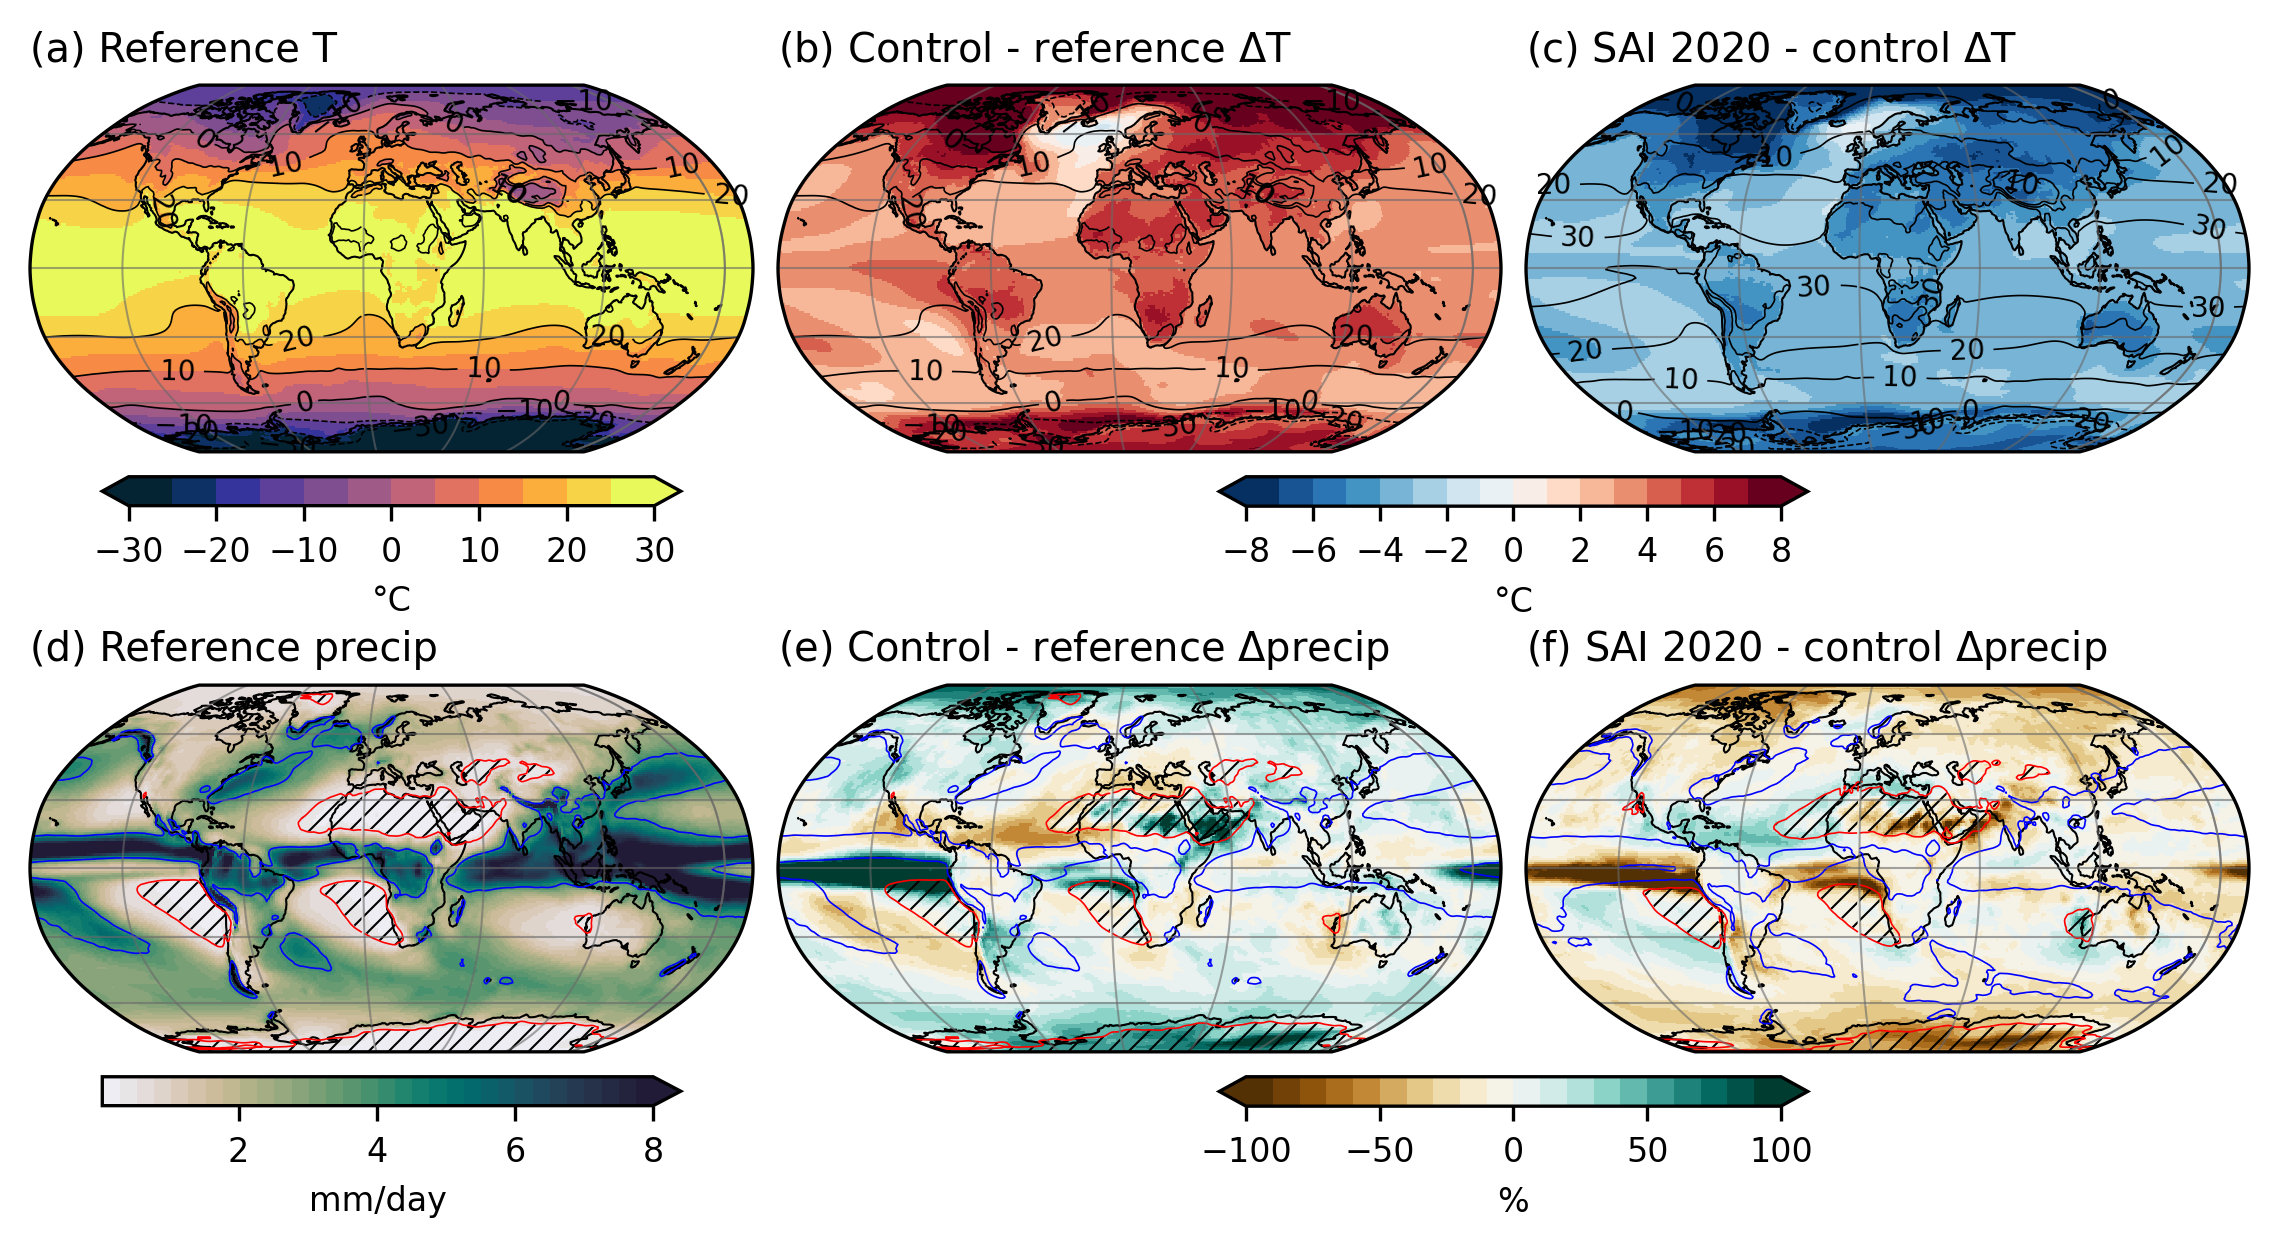
\includegraphics[width=0.95\linewidth]{images/CAM_scens.png}
	\caption{CAM model results; (a): Reference annual mean 2-meter temperature. (b): Annual mean 2-meter temperature anomaly for Control compared to Reference, Reference shown in black contours in 10°C intervals (c): Annual mean 2-meter temperature anomaly for SAI 2020 compared to Control, contours as in (b) but for Control. (d): Reference annual mean precipitation in mm/day, 4 mm/day shown in blue contours, $<0.3$mm/day shown in red contours with hatching. (e) Annual mean precipitation anomaly for Control compared to Reference, contours as in (d). (f): Annual mean precipitation anomaly for SAI 2020 compared to Control, contours as in (d) but for Control.}
	\label{fig:CAM_scens}
\end{figure}


\subsection{SAI 2020 2-meter Temperature Anomalies in CAM and WACCM}
The annual and seasonal mean 2-meter temperature anomalies of SAI 2020 compared to the Reference for CAM and WACCM are shown in Figure \ref{fig:TREFHT_20ref}. Figure \ref{fig:TREFHT_20ref}(c) shows the difference between (a) and (b), i.e. the inter-model difference corrected for their difference in SAI 2020. Figures \ref{fig:TREFHT_20ref}(f) and (i) show the annual and seasonal zonal mean anomalies for CAM and WACCM respectively. 

The annual mean anomalies in Figures \ref{fig:TREFHT_20ref}(a) and (b) show a generally similar pattern of warming over the tropics, cooling over the subtropics and warming over the poles. The Arctic warms more in CAM than it does in WACCM, at most 3°C. Both models show significant cooling over the nothern Atlantic Ocean, again resembling the North Atlantic warming hole seen in Figure \ref{fig:CAM_scens}, CAM more so than WACCM. The El Ni\~no pattern in the eastern Atlantic is visible in both models, though more pronounced in CAM. 

Figure \ref{fig:TREFHT_20ref}(c) confirms the patterns described above. The figure also highlights the difference in response over North America and off the coast of Antarctica between 0° and 30°E, where CAM slightly cools and WACCM slightly warms, leading to a significant difference.

In Figures \ref{fig:TREFHT_20ref}(d) and (e), the seasonal response of CAM is shown. Comparison between the two seasons and the annual mean shows that most warming at the poles occurs during their respective winter. This is further confirmed by the zonal mean anomaly in Figure \ref{fig:TREFHT_20ref}(f). The El Ni\~no pattern is stronger in magnitude in JJA, though more expansive in DJF, though this is not visible in the zonal mean anomaly. 

The same patterns are visible in Figures \ref{fig:TREFHT_20ref}(a) and (b), with the Antarctic as a whole warming in the Southern Hemisphere winter and the Barentsz sea in the Arctic warming significantly in the Northern Hemisphere winter. This pattern is confirmed by Figure \ref{fig:TREFHT_20ref}. 

\begin{figure}[H]
	\centering
	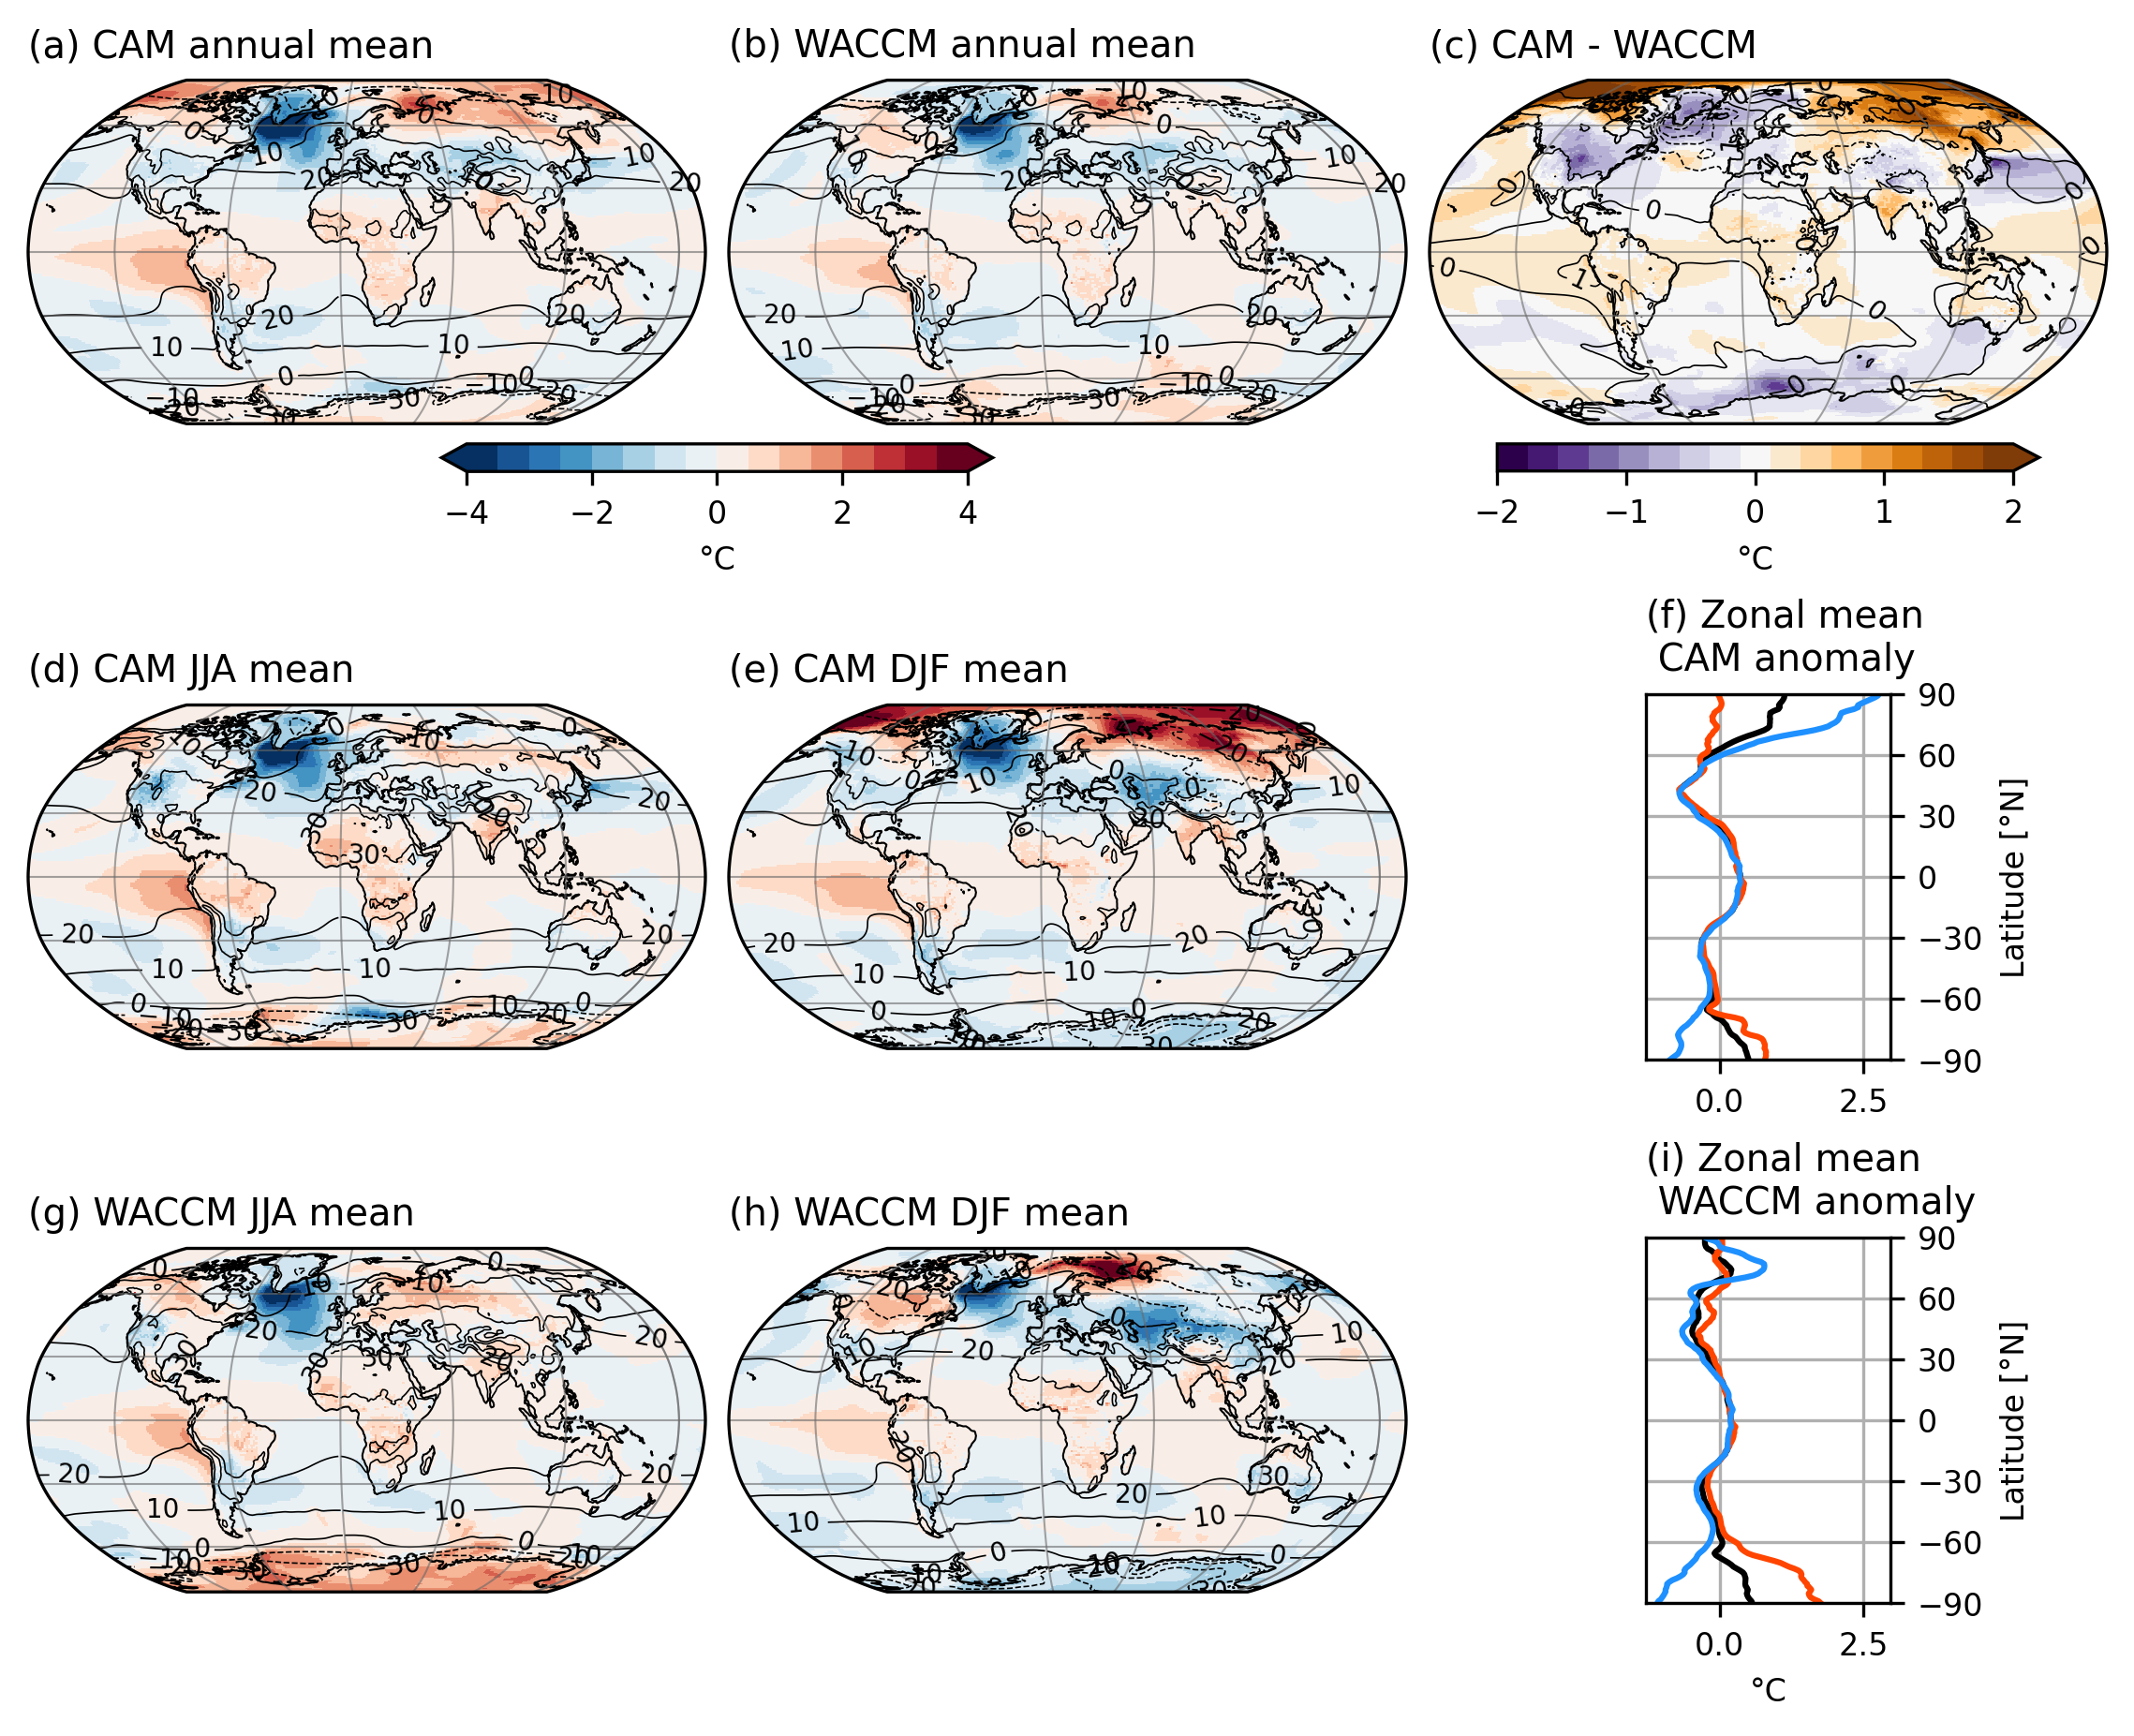
\includegraphics[width=0.95\linewidth]{images/TREFHT_20ref.png}
	\caption{(a,b): Annual mean 2-meter temperature anomalies of SAI 2020 compared to Reference in (a) CAM and (b) WACCM. Reference mean temperature shown in black contours in 10°C intervals. (c): Difference between CAM and WACCM temperature anomalies. WACCM anomaly shown in black contours in 1°C intervals. (d,e): CAM anomalies as in (a,b) for (d) JJA and (e) DJF. (f): CAM zonal average temperature anomaly as in (a,b), annual mean anomaly in black, JJA anomaly in red, DJF anomaly in blue. (g,h,i): analogous to (d,e,f) for WACCM.}
	\label{fig:TREFHT_20ref}
\end{figure}


\subsection{SAI 2020 Precipitation Anomalies in CAM and WACCM}
The annual and seasonal mean precipitation anomalies of SAI 2020 compared to Reference for CAM and WACCM are shown in Figure \ref{fig:PRECT_20ref}. Figure \ref{fig:PRECT_20ref}(c) shows the difference between (a) and (b) as above in Figure \ref{fig:TREFHT_20ref}, note that this difference is calculated in percentage points. Figures \ref{fig:PRECT_20ref}(f) and (i) show the annual and seasonal zonal mean anomalies for CAM and WACCM respectively. 

The annual mean anomalies in Figures \ref{fig:PRECT_20ref} and \ref{fig:PRECT_20ref} show a similar pattern overall, with a small decrease in precipitation over most of the globe and larger increase in dry areas and the tropics. CAM shows a much larger precipitation increase over the eastern Pacific Ocean, with a southward shift of the ITCZ, while WACCM shows a larger increase over dry areas like the Arabian Peninsula. 

The same patterns are observed in the seasonal precipitation anomalies in Figures \ref{fig:PRECT_20ref}(d), (e), (g) and (h), with the exception of southern Brazil, where CAM shows a larger increase than WACCM in the JJA mean. The zonal mean anomalies in Figures \ref{Figure}(f) and (i) also show that precipitation in the ITCZ increases twice as much in CAM compared to WACCM. The increase in the Arctic is also about twice as high in CAM as it is in WACCM, while the Antarctic shows the opposite. 

The observerd precipitation trends correlate with the observed 2-meter temperature trends, in both the annual and seasonal results. A higher 2-meter temperature increase correlates to a higher precipitation increase, most notably in the eastern Pacific Ocean and the Arctic and Antarctic. 

\begin{figure}[H]
	\centering
	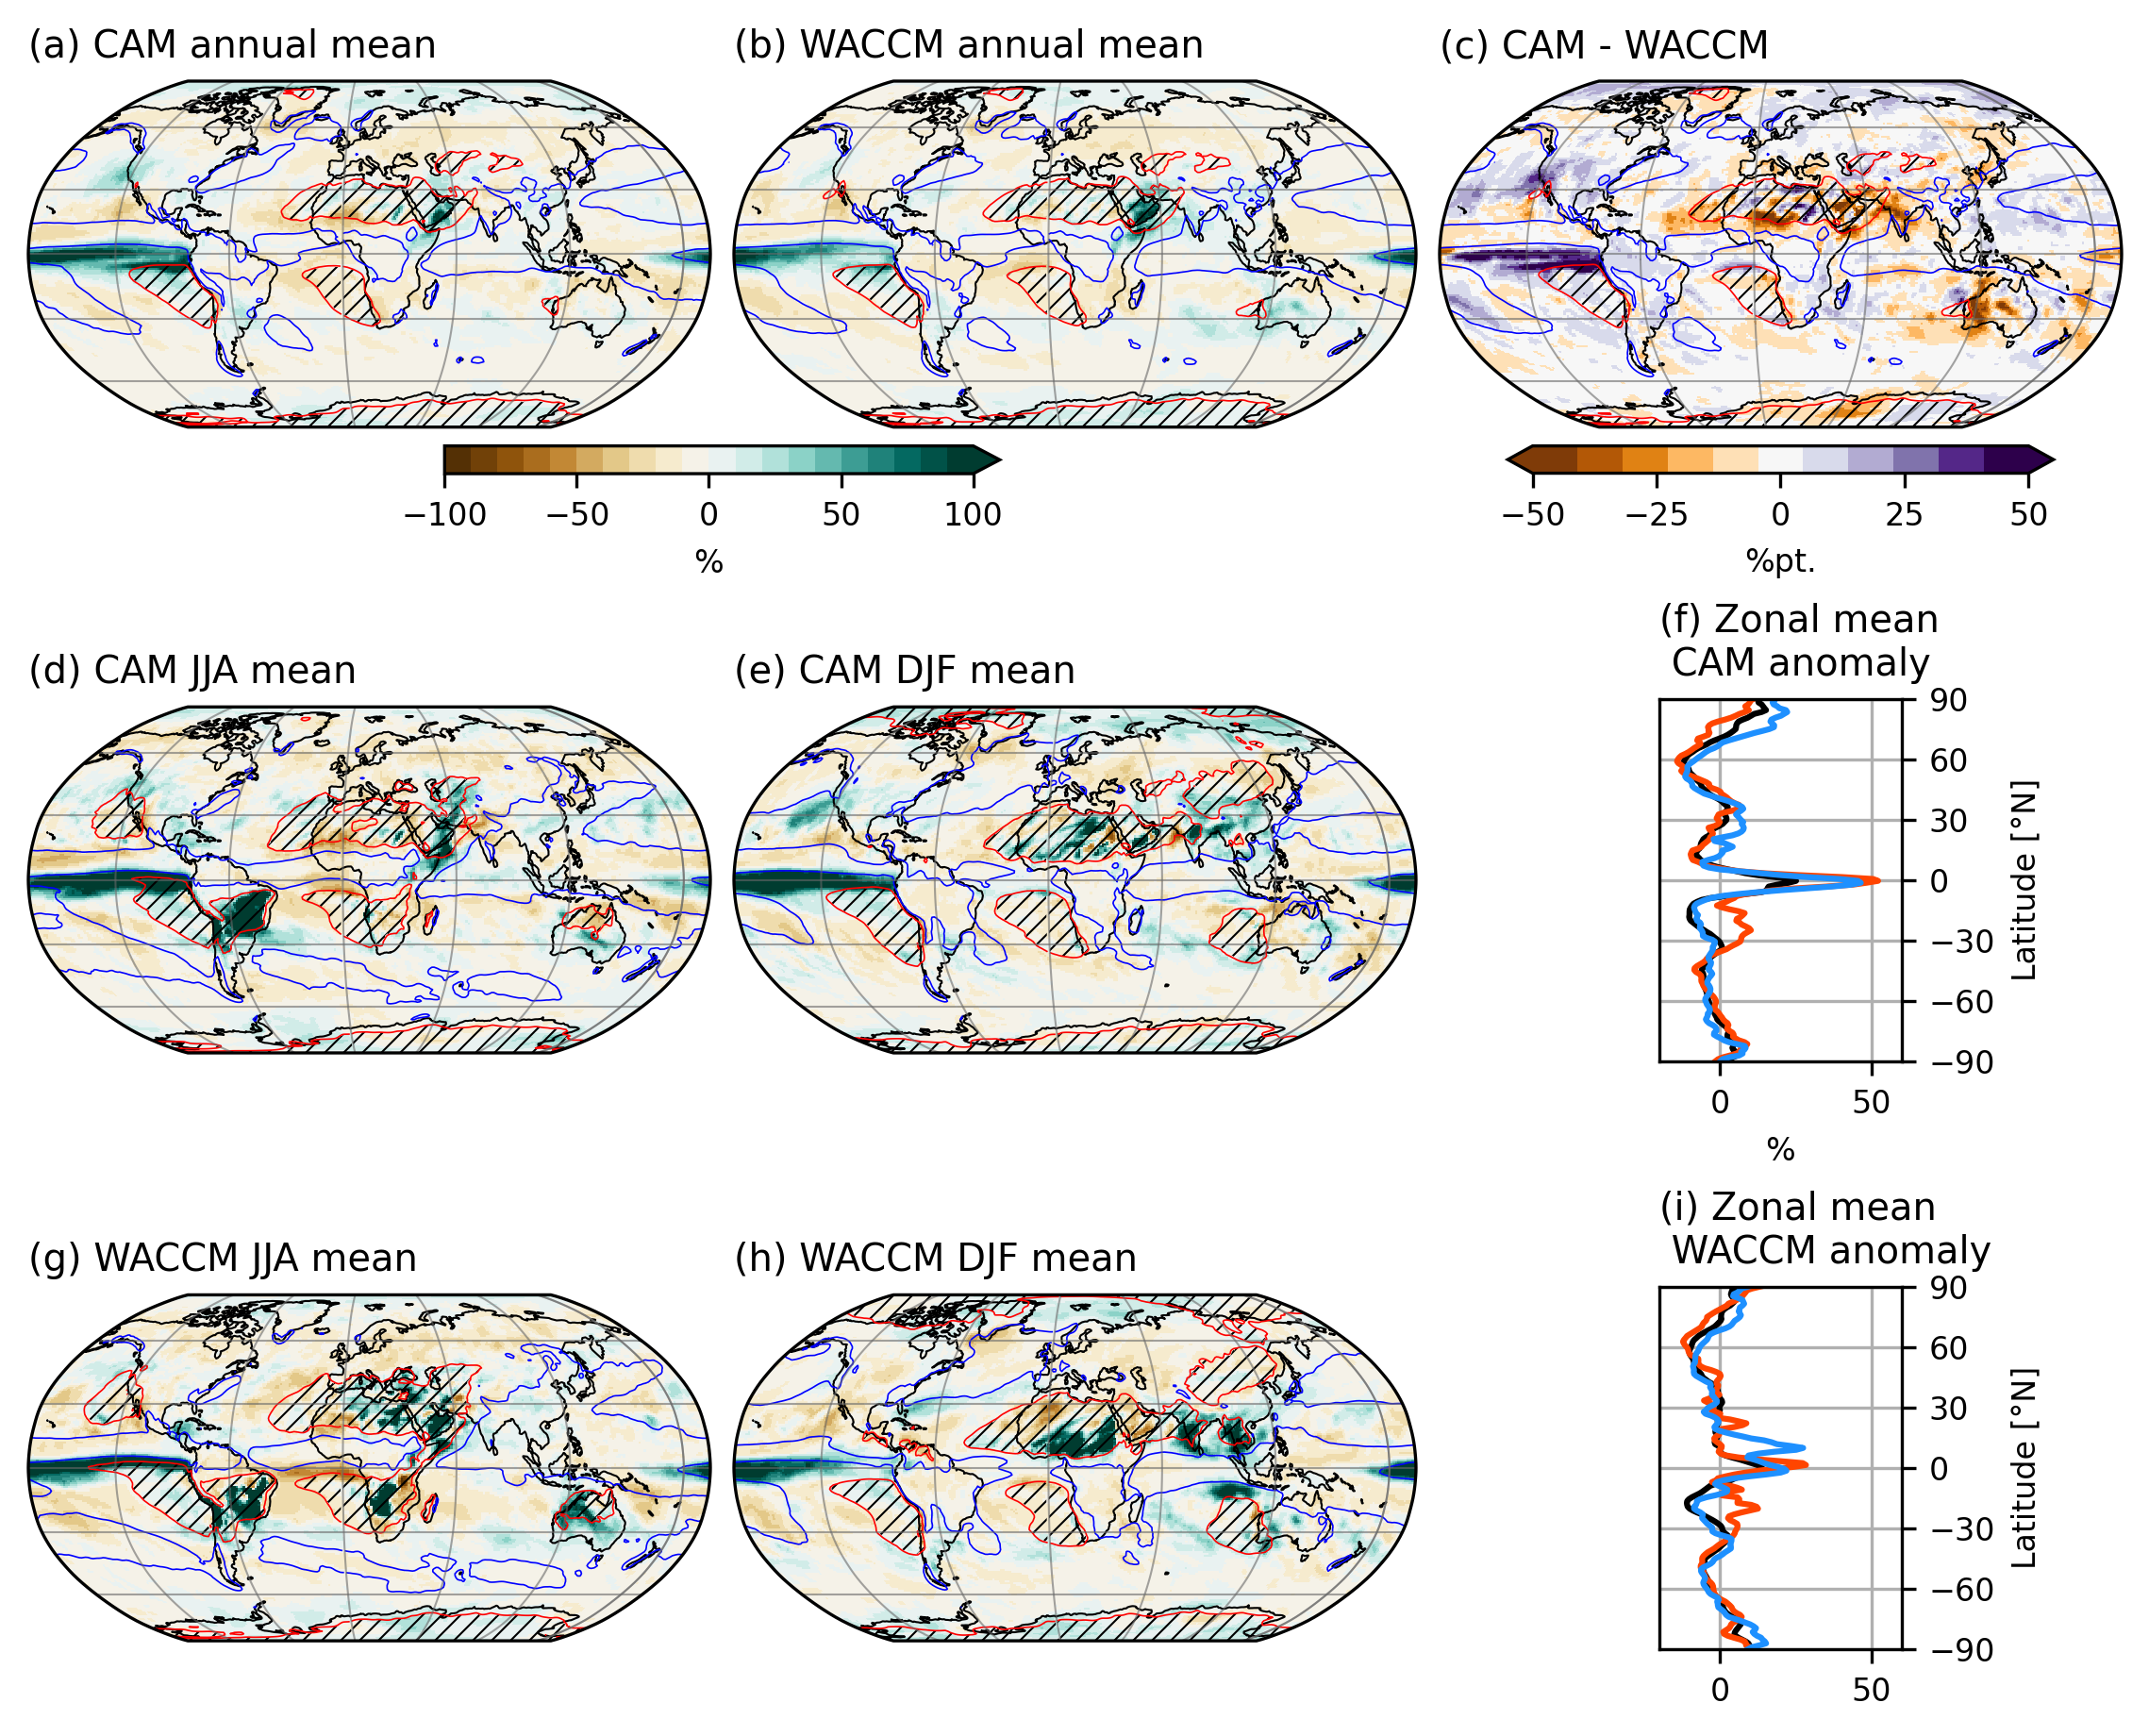
\includegraphics[width=0.95\linewidth]{images/PRECT_20ref.png}
	\caption{(a,b): Annual mean precipitation anomalies of SAI 2020 compared to Reference in (a) CAM and (b) WACCM. Reference mean precipitation shown, 4 mm/day in blue, $<0.3$mm/day in red with hatching. (c): Difference between CAM and WACCM precipitation anomalies. WACCM Control mean precipitation as in (b). (d,e): CAM anomalies as in (a,b) for (d) JJA and (e) DJF. (f): CAM zonal average precipitation anomaly as in (a,b), annual mean anomaly in black, JJA anomaly in red, DJF anomaly in blue. (g,h,i): analogous to (d,e,f) for WACCM.}
	\label{fig:PRECT_20ref}
\end{figure}


\subsection{Absolute temperature and precipitation differences between CAM and WACCM}
The absolute temperature differences for Reference, Control and SAI 2020 are shown in \ref{fig:CAM_WACCM}. The 2-meter temperature difference reveals that CAM is much warmer than CAM on the Northern Hemisphere, with the largest difference in the Arctic where the difference exceeds 7° in Reference and SAI 2020. In contrast, CAM is slightly cooler in the Southern Hemisphere, with the difference being generally less than 2°C except for a few areas in Reference.

This difference is lesser in Control, but still a clear difference between the two hemispheres is visible. The difference is worsened in SAI 2020, with the Arctic warming much more in CAM than in WACCM. 

As for precipitation, there is a small difference in Reference, with cam being slighly wetter over the tropics and dryer over the western Pacific Ocean. Differences shift in Control, with most notably a stark increase in precipitation over the eastern Pacific Ocean in CAM compared to WACCM. The same is seen in SAI 2020, with the ITCZ also shifting more clearly southward in CAM compared to WACCM. 

\begin{figure}[H]
	\centering
	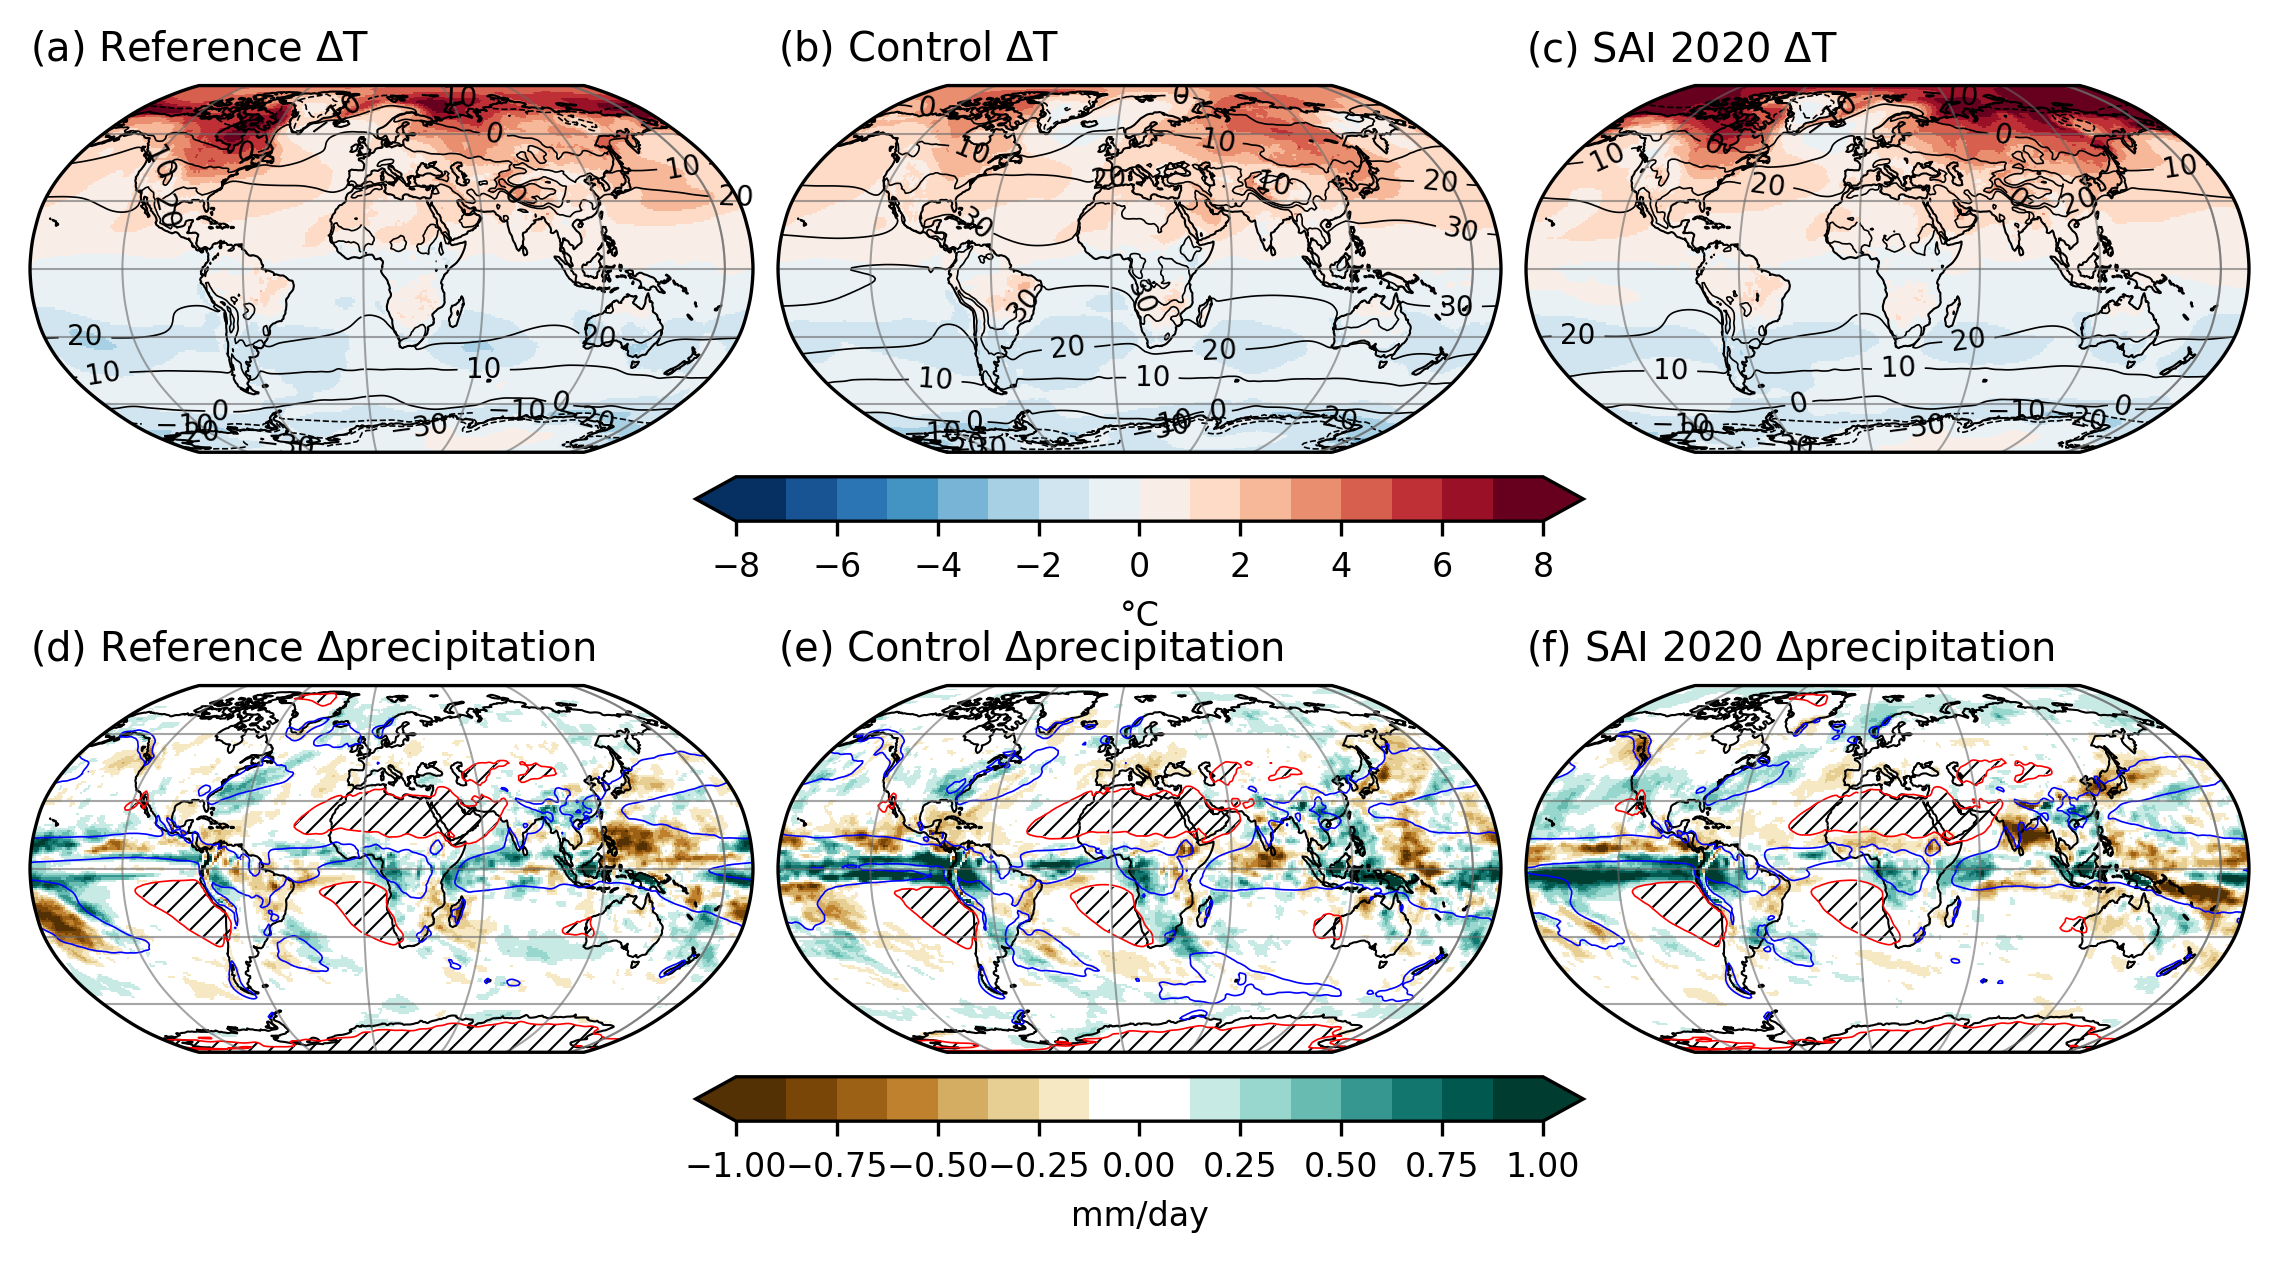
\includegraphics[width=0.95\linewidth]{images/CAM_WACCM.png}
	\caption{(a-c): Reference, Control and SAI 2020 CAM-WACCM 2-meter temperature differences, WACCM temperature in black contours in 10°C intervals. (d-e): Analogous to (a-c) for precipitation, 4 mm/day in blue contours, $<0.3$ mm/day in red contours with hatching.}
	\label{fig:CAM_WACCM}
\end{figure}


\subsection{SAI 2020 Potential Temperature and Zonal Wind Anomalies in CAM and WACCM}
The zonal mean potential temperature $\theta$ anomaly and the zonal mean zonal wind anomaly for CAM and WACCM is shown in Figure \ref{fig:th_U_full}, for both the annual and seasonal mean. 
In Figures \ref{fig:th_U_full}(a)-(f) the potential temperature anomaly shows significant warming in the stratosphere, in a pattern reminiscent of the aerosol field from section \ref{emulator_pt1}. The warming extends to the poles only in the summer hemisphere, due to the poles only receiving solar radiation in their respective summer. The cooling observed in CAM over the Arctic in winter is not observed in WACCM at the same magnitude, any cooling extends to about the same altitude, but is not as severe as it is in CAM. CAM also shows more cooling than WACCM in the Antarctic winter, though the difference is not as stark as in the Arctic. The cooling effect of greenhouse gases in the upper stratosphere is visible in CAM and WACCM in the annual and seasonal means. There is no significant potential temperature change observed below about 300 hPa. 

The zonal mean zonal wind anomaly in Figures \ref{fig:th_U_full}(g)-(l) shows a large increase in zonal winds in the upper stratosphere in both hemispheres. The seasonal mean figures reveal that most zonal wind increase occurs in the winter hemisphere. The polar night jet (PNJ) forms in the upper stratosphere in winter, driven by the large latitudinal temperature gradient during the polar night. The peak increase in the winter hemisphere is observed above the area with the largest increase in the latitudinal temperature gradient, see Figures \ref{fig:th_U_full}(b), (c), (e) and (f), discussed above. The largest anomaly is visible on the equator side of the PNJ, indicating an increase in strenght and an equatorward shift. This pattern is observed everywhere, except in the Arctic winter in WACCM (Fig. \ref{fig:th_U_full}(l)). The PNJ only increases in strength slightly, correlating to the temperature anomaly (Fig. \ref{fig:th_U_full}(f)). 

Lower statospheric and tropospheric winds are largely unchanged in both CAM and WACCM, with only significant changes reaching the surface in the Arctic winter in CAM. 

\begin{figure}[H]
	\centering
	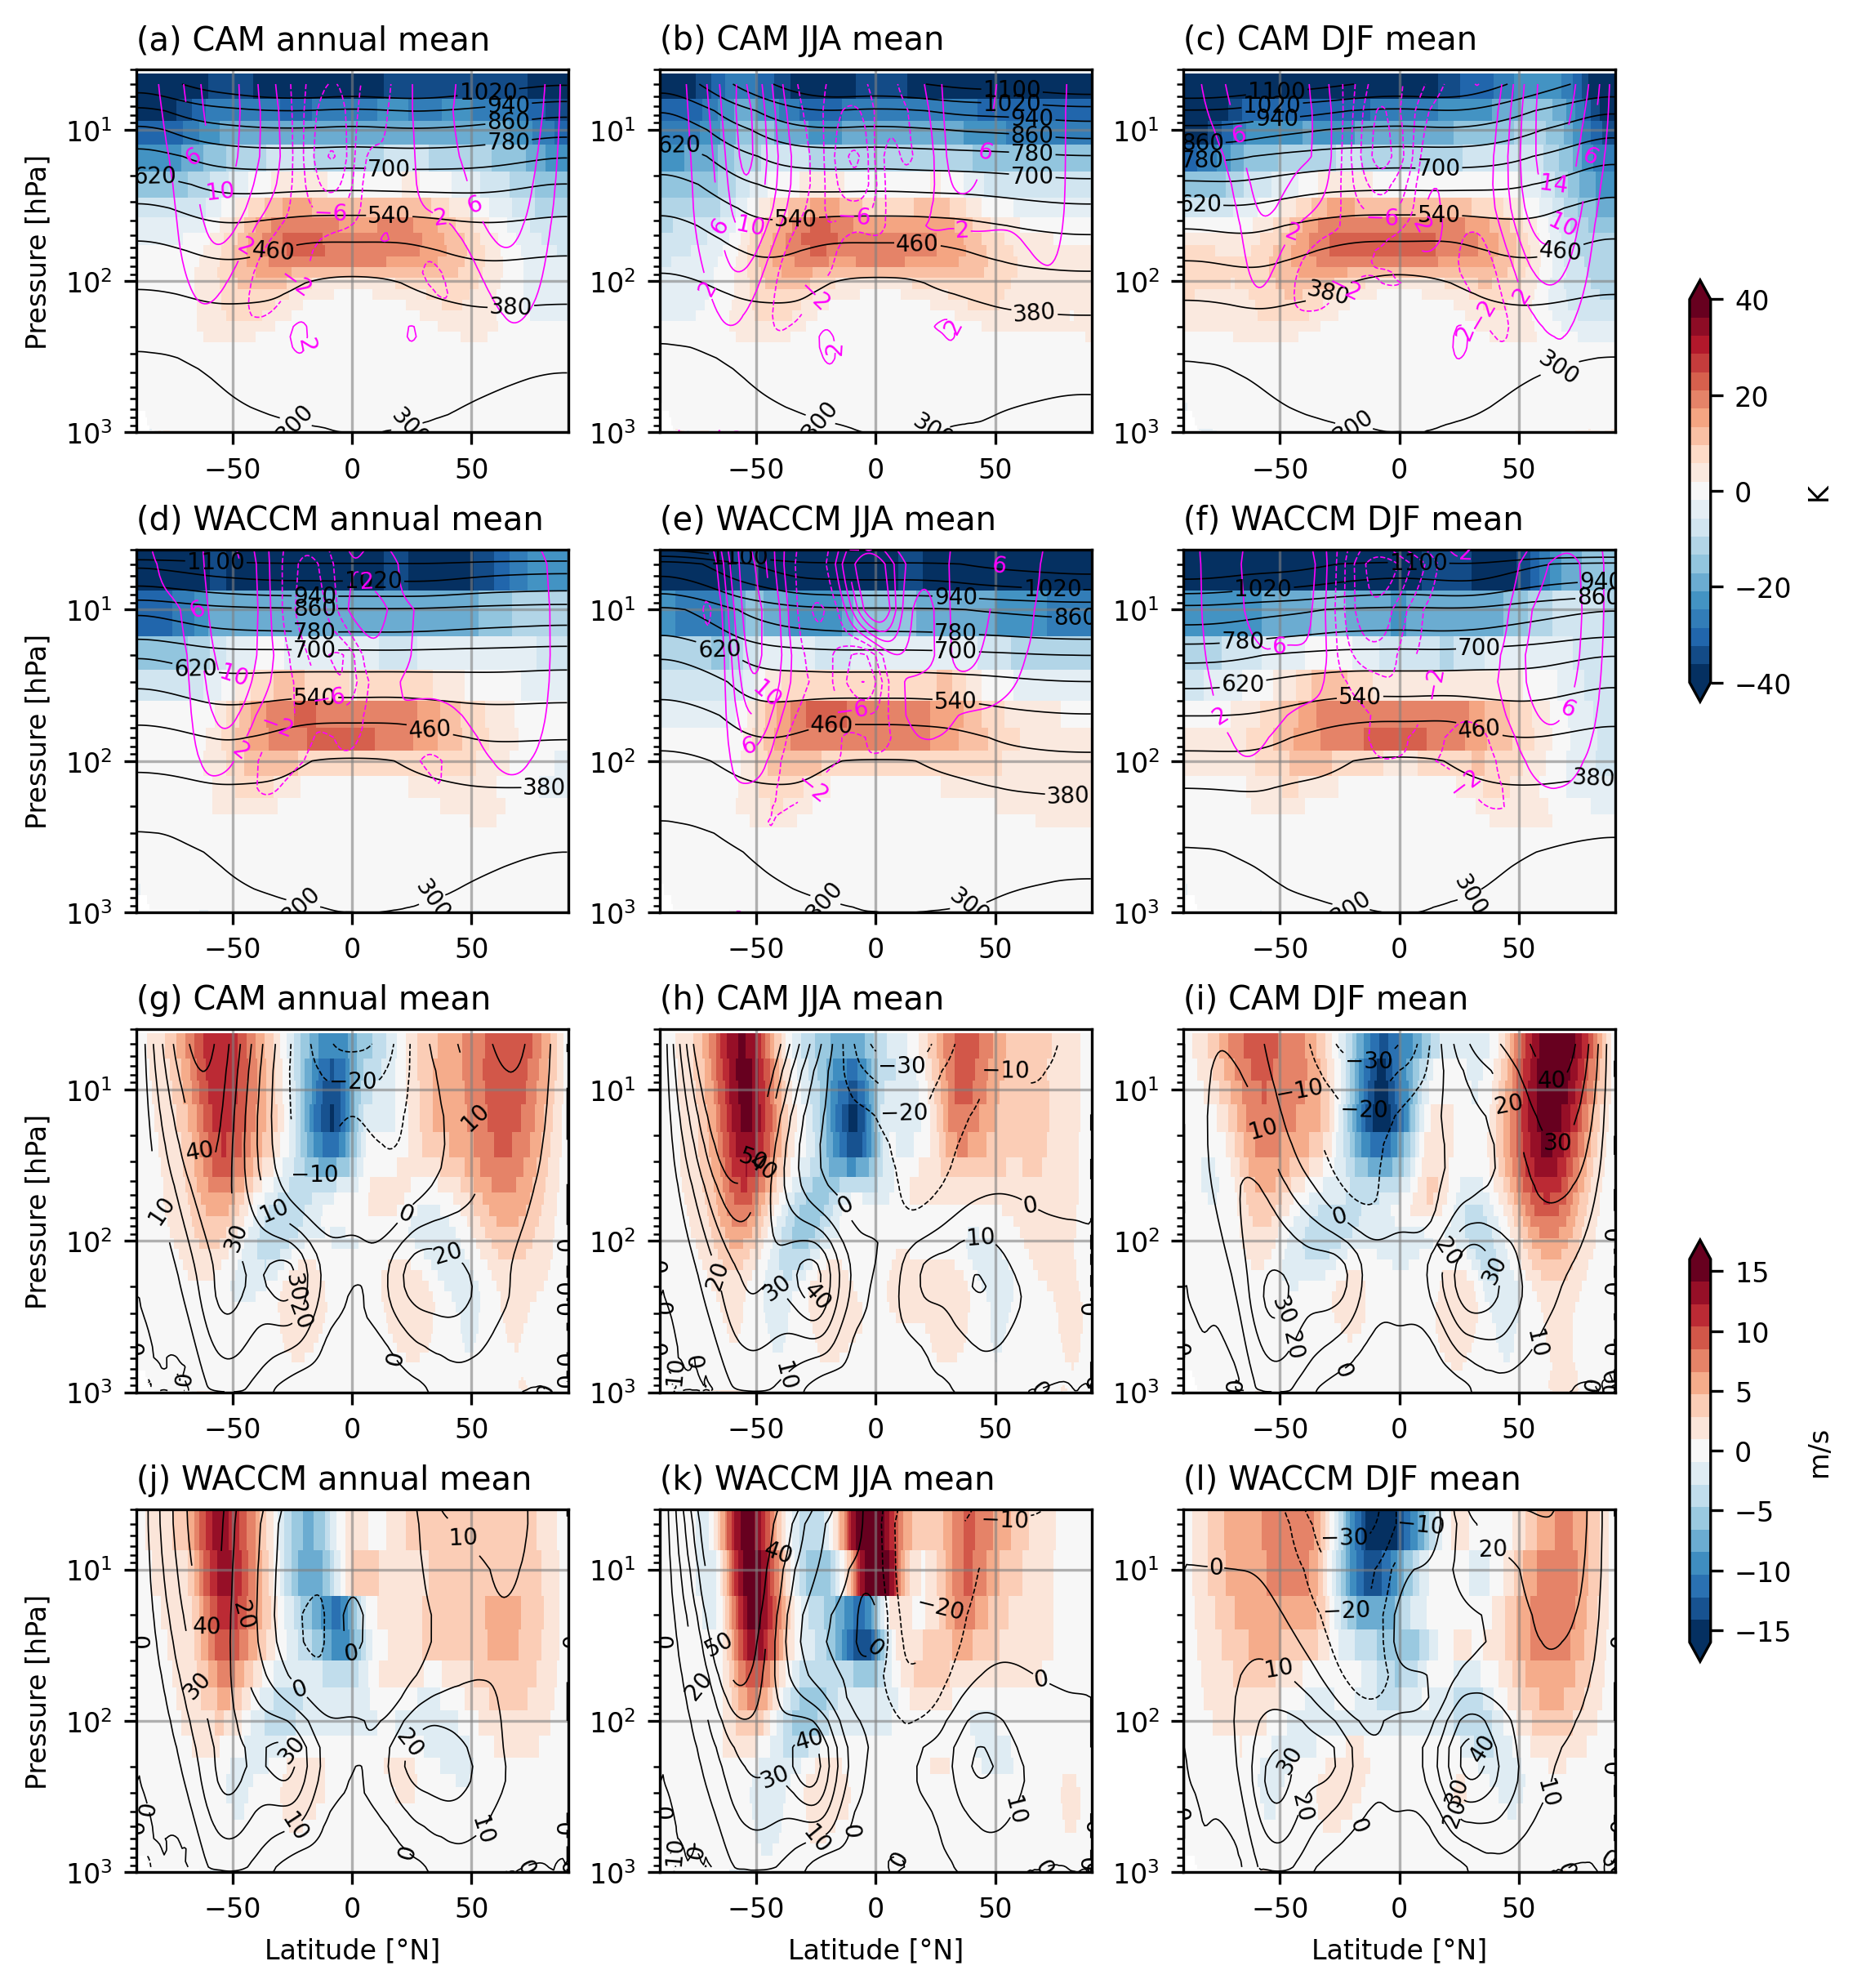
\includegraphics[width=0.95\linewidth]{images/th_U_full.png}
	\caption{(a-f): Zonal mean potential temperature anomaly for (a-c) CAM and (d-f) WACCM, annual, JJA and DJF mean shown for both models. Reference potential temperature shown in black contours, zonal mean zonal wind anomalies shown in magenta contours. (g-l): Zonal mean zonal wind anomaly for WACCM and CAM analogous to (a-f), Reference zonal wind shown in black contours.}
	\label{fig:th_U_full}
\end{figure}
\newpage

\part{Southern Hemisphere Atmospheric Circulation}
\section{Methods Part II}
\subsection{Scenarios Used for the Simulations}
All simulations considered in this second part were extended to 2130, where the forcing was kept constant at the 2100 levels. This extension provides further insight in the long-term effects of deploying SAI. Especially in the rapid cooling SAI scenario the extension provides time for the climate system to adjust to the `shock' it experienced from SAI. 

The rapid cooling experiment is branched from the SSP5-8.5 simulation in 2080, SAI is then deployed to restore temperatures to 2020 levels. The control algorithm is adjusted for the first up to six years to prevent extremely high aerosol concentrations that would result in too rapid cooling. 

Shown in Figure \ref{fig:Tgrad_ext} are the temperature targets from \ref{eq:Tpsi} for the SSP5-5.8, gradual SAI and rapid cooling SAI simulations. After about 10 years of SAI the $T_0$ target is reached and maintained, like in the gradual SAI simulation. However, in contrast to the gradual SAI simulation, the rapid cooling SAI simulation is not able to return to and then maintain 2020 levels for $T_1$ and $T_2$. In the rapid cooling SAI simulation both targets are overshot, though their levels are stabilised after 2100. 

\begin{figure}[h]
	\centering
	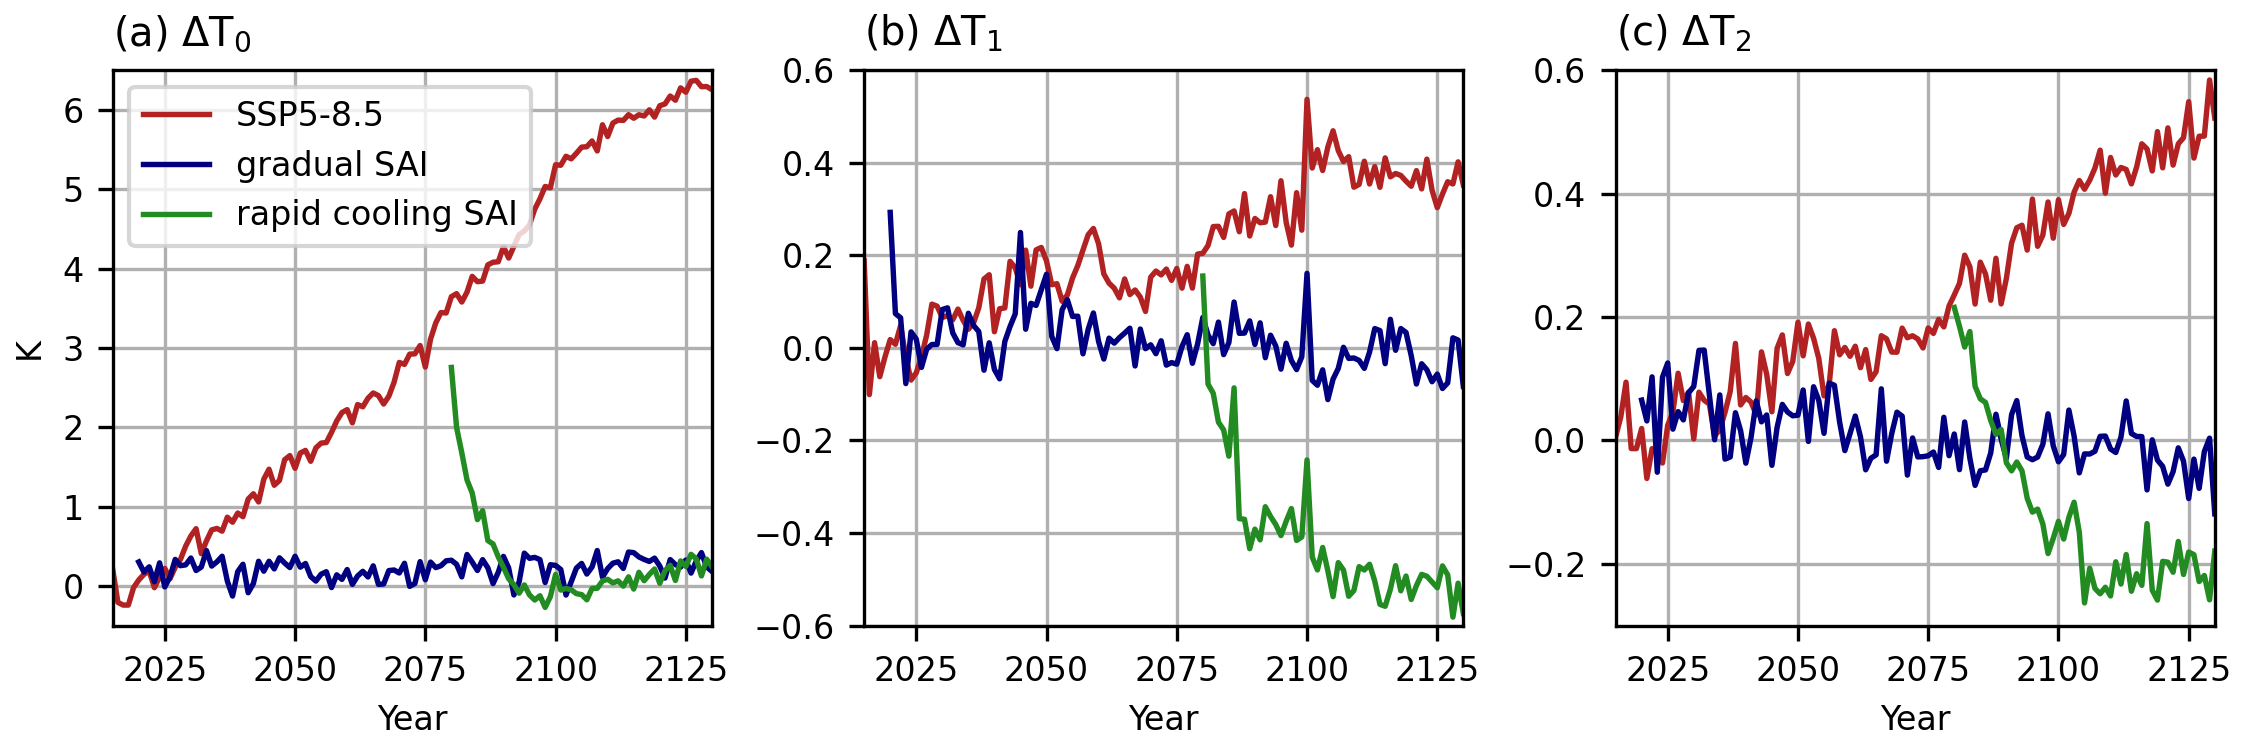
\includegraphics[width=\linewidth]{images/Tgrad_ext.png}
	\caption{Deviatons from temperature targets $T_0$, $T_1$, $T_2$ as compared to 2016-2025 mean, for Control, SAI 2020 and SAI 2080 scenarios in CAM.}
	\label{fig:Tgrad_ext}
\end{figure}


\subsection{Definition of Scenarios and Time Periods for Part II}
The two simulations from Part I are referred to in the same way in this second part, namely the SSP5-8.5 simulation and the gradual SAI simulation. The simulation with the rapid cooling experiment is referred to as the rapid cooling SAI simulation. 

Throughout this second part, four time periods are selected to visualise and interpret the results from the simulations. As in part I, for each period the 20-year mean is taken, unless specified otherwise. These periods are defined as follows:

\begin{itemize}
    \item \textbf{Reference} The period 2016-2035 of the SSP5-8.5 simulation.
    \item \textbf{Control} The period 2111-2130 of the SSP5-8.5 simulation.
    \item \textbf{SAI 2020} The period 2111-2130 of the gradual SAI simulation.
    \item \textbf{SAI 2080} The period 2111-2130 of the rapid cooling SAI simulation.
\end{itemize} % tabel van maken


\subsection{Thermal Wind}
To calculate thermal winds from the temperature gradients, the thermal wind balance equation is used. As the vertical layers of the model are converted to pressure coordinates, the equation takes the form 

\begin{equation}
    \frac{\partial v_g}{\partial p} = - \frac{R}{pf_0} \frac{\partial T}{\partial x};\ 
    \frac{\partial u_g}{\partial p} = \frac{R}{pf_0} \frac{\partial T}{\partial y},
\end{equation}

where $v_g$,$u_g$ is the geostrophic wind in meridional and zonal directions respectively, $R = 286.9$ J kg$^{1}$ K$^{1}$ is the specific gas constant for dry air, $p$ is pressure, $f_0 = 2\Omega \sin \varphi$ is the coriolis parameter at the chosen reference latitude $\varphi$, $\frac{\partial T}{\partial x,y}$ is the layer-mean temperature gradient in zonal and meridional direction respectively. Rewriting and integrating gives us

\begin{equation}
    \begin{split}
        \int\displaylimits_{p_0}^{p_1} \partial v_g &= \int\displaylimits_{p_0}^{p_1} - \frac{R}{f_0} \frac{\partial T}{\partial x} \partial \ln p; \\
        \int\displaylimits_{p_0}^{p_1} \partial u_g &= \int\displaylimits_{p_0}^{p_1} \frac{R}{f_0} \frac{\partial T}{\partial y} \partial \ln p,
    \end{split}
\end{equation}

where $p_{0,1}$ are the lower and upper boundaries of the model layer, respectively, so that $p_1 < p_0$. Because $T$ is the layer-mean temperature and $R$ and $f_0$ are constants, we can evaluate this integral to find the thermal wind in the layer between $p_0$ and $p_1$

\begin{equation}
    \begin{split}
        v_T = v_g(p_1) - v_g(p_0) &= \frac{R}{f_0} \frac{\partial T}{\partial x} \ln\left(\frac{p_0}{p_1}\right);\\
        u_T = u_g(p_1) - u_g(p_0) &= - \frac{R}{f_0} \frac{\partial T}{\partial y} \ln\left(\frac{p_0}{p_1}\right).
    \end{split}
\end{equation}

To increase stability in our calculations, we assume that the thermal wind below 850 hPa is equal to the model wind, because the thermal wind calculation in the layers below that will most likely not produce stable results. To then find the thermal wind at a given pressure coordinate above 850 hPa, we take the cumulative sum of the thermal wind from 850 hPa up to the given pressure plus the meridional or zonal wind of the layer below 850 hPa ($v(p_{-1}),u(p_{-1})$). This gives us for the thermal wind at pressure coordinate $p_i$ 

\begin{equation}
    \begin{split}
        v_{T}(p_i) &= v(p_{-1}) + \frac{R}{f_0} \sum_{i=0}^{i} \frac{\partial T_i}{\partial x} \ln \left(\frac{p_i}{p_{i+1}}\right),\\
        u_{T}(p_i) &= u(p_{-1}) + \frac{R}{f_0} \sum_{i=0}^{i} - \frac{\partial T_i}{\partial y} \ln \left(\frac{p_i}{p_{i+1}}\right).
    \end{split}
\end{equation}


\subsection{Kinetic Energy and Eddy Kinetic Energy}
The CAM model woks with wind in the form of $u = \overline{u} + u^{\ast}$, $v = \overline{v} + v^{\ast}$, with $u,v$ the total wind, $\overline{u},\overline{v}$ the monthly-mean wind and $u^\ast,v^\ast$ the deviation from the mean wind. The model output contains monthly averages $\overline{u},\overline{v}$ and $\overline{u^2},\overline{v^2}$. % check in CESM documentation

The kinetic energy $KE$ per unit mass can thus be found from the model results directly through

\begin{equation}\label{eq:KE}
    KE = \frac{1}{2} \left( \overline{u^2} + \overline{v^2} \right).
\end{equation}

The eddy kinetic energy $EKE$ per unit mass can be found through 

\begin{equation}\label{eq:EKE}
    EKE = \frac{1}{2} \left( \overline{u^{\ast 2}} + \overline{v^{\ast 2}} \right),
\end{equation}

\noindent with $\overline{u^{\ast 2}}, \overline{v^{\ast 2}}$ found through
\begin{equation}
    \begin{split}
        \overline{u^2} &= \overline{\left( \overline{u} + u^\ast \right) \left( \overline{u} + u^\ast \right)},\\
        &= \overline{\overline{u}^2 + 2 \overline{u}u^\ast + u^{\ast 2}},\\
        &= \overline{u}^2 + \overline{u^{\ast 2}} \Rightarrow \overline{u^{\ast 2}} = \overline{u^2} - \overline{u}^2, 
    \end{split}
\end{equation}

which can be found with the model output. 

To find the kinetic and eddy kinetic energy per unit volume, we multiply the results from Eq. \ref{eq:KE} and \ref{eq:EKE} with the local density. Assuming an ideal gas, we approximate the density through
\begin{equation}
    \rho = \frac{p}{RT},
\end{equation}
\noindent with $p$ pressure, $T$ temperature and $R$ again the specific gas constant for dry air. 


\subsection{Jet Intensity Maps}
The jet intensity maps are made by counting the number of times the zonal wind or eddy kinetic energy surpasses a set threshold. Each timestep and coordinate is evaluated individually, after which the set is summed over time and the vertical dimension. This result is then normalised by the number of timesteps multiplied by the number of vertical model levels included in the analysis. This results in a fraction that represents the time and vertical extent of the atmospheric jet. 

To visualise the Polar night jet (PNJ), in the upper stratosphere, and the subtropical jet (STJ), in the lower stratosphere, this method is applied to the zonal wind fields. For the eddy-driven jet (EDJ), also in the lower stratosphere, this method is applied to the eddy kinetic energy fields. 

\newpage

\section{Results Part II: Lower Stratosphere}\label{lowerstrat}
This section contains the results for the SSP5-8.5, the gradual SAI and the rapid cooling SAI experiments, focusing on the atmospheric dynamics of the lower stratosphere.

\subsection{Potential temperature and Zonal Wind Anomaly}
The zonal mean potential temperature and potential temperature anomalies for Control, SAI 2020 and SAI 2080 are shown in Figures \ref{fig:th_U_zmdiff_full} (annual mean), \ref{fig:th_U_zmdiff_full} (JJA) and \ref{fig:th_U_zmdiff_full} (DJF). The countours indicate the zonal mean zonal wind and zonal mean zonal wind anomalies. 

In Control we see the potential temperature anomaly signature of increased greenhouse gases, with warming at the surface and the troposphere, extending to the lower stratosphere and cooling in the upper stratosphere. In both SAI periods the potential temperature increases where SAI is deployed in the lower stratosphere, with the surface and troposphere showing no significant change. The anomaly in SAI 2020 is about 2.5°C larger than SAI 2080. In both SAI experiments the upper stratosphere shows the potential temperature decrease from greenhouse gases also observed in Control. 

The seasonal mean potential temperature anomalies show a larger increase in the summer over the Antarctic. In winter the latitudinal potential temperature gradient is larger, because the Antarctic receives no solar radiation during the polar night. 

The zonal mean zonal wind anomalies show that the most drastic changes in atmospheric dynamics occur in winter (JJA), thus we will focus on this season in our analysis of the lower stratosphere.

In Figure \ref{fig:th_U_zmdiff_JJA} the zonal mean of the zonal component of the thermal wind is shown, together with the observed zonal mean zonal wind in red countours. The observed wind and thermal wind show very similar patterns, with the observed wind consistently lower than the calculated thermal due to friction effects. The largest changes occur in the upper stratosphere, affecting the polar night jet, this will be discussed in section \ref{upperstrat}. 


\begin{figure}[H]
	\centering
	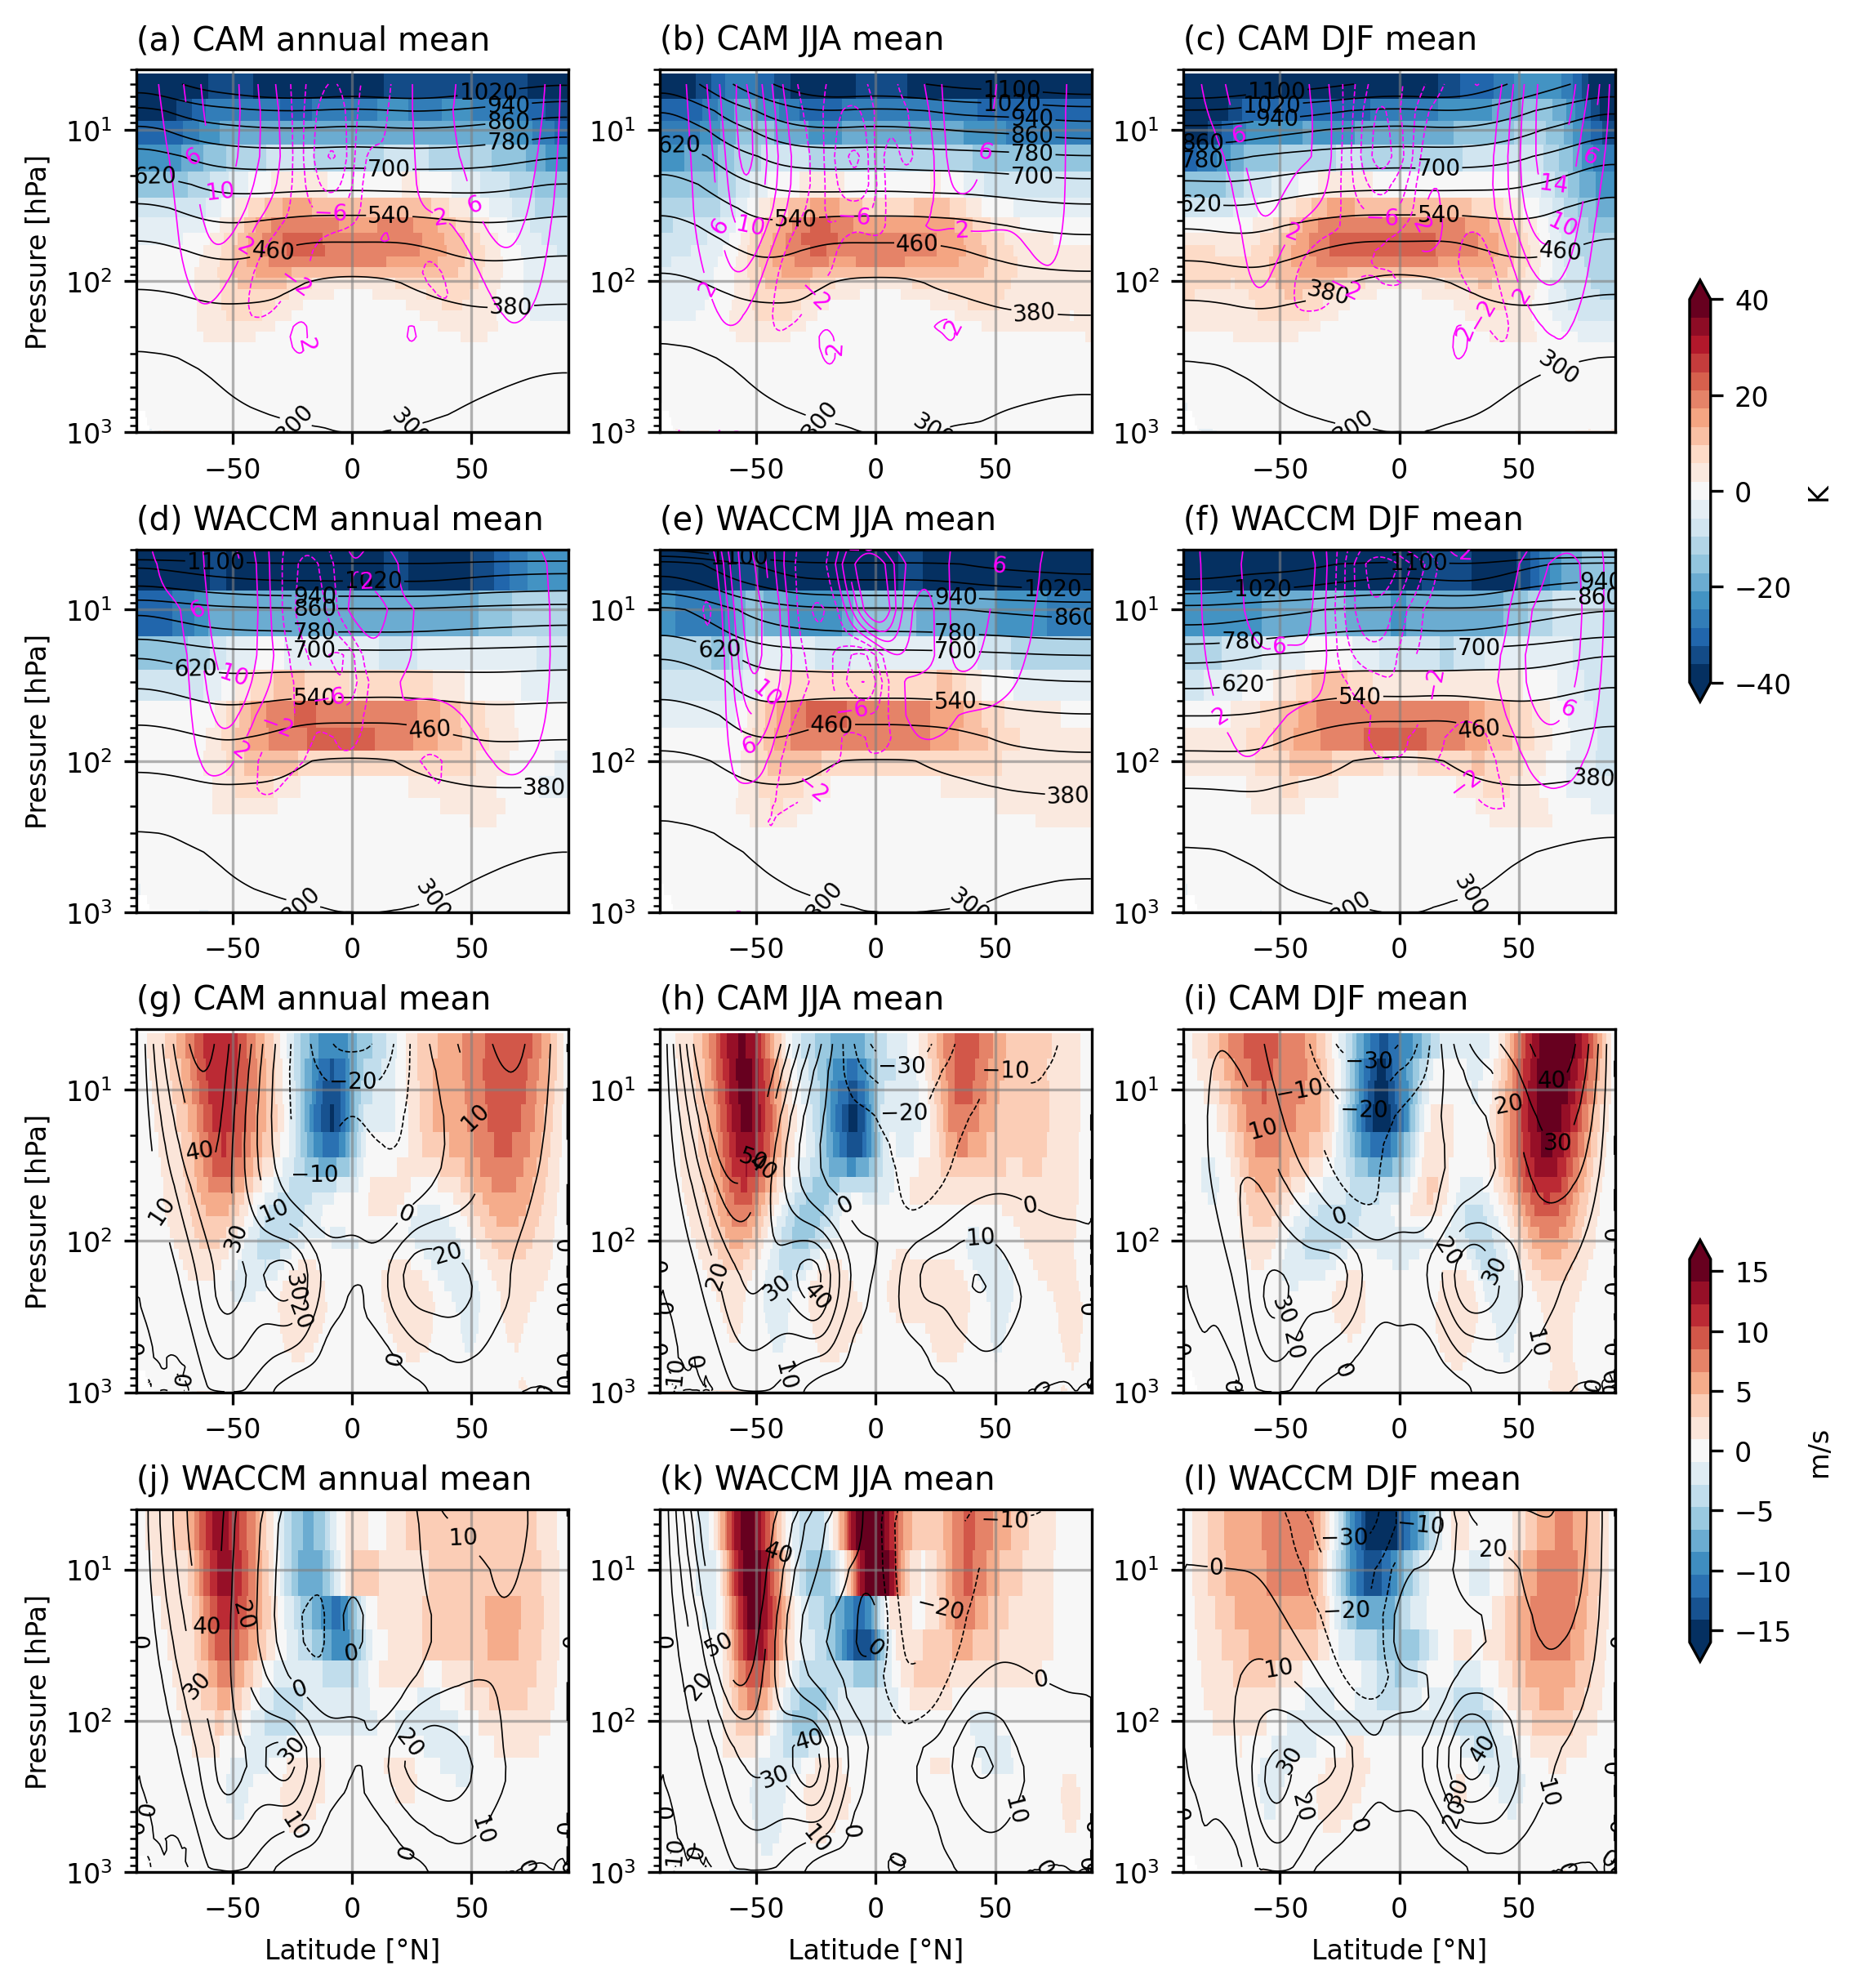
\includegraphics[width=0.95\linewidth]{images/th_U_full.png}
	\caption{Annual mean zonal mean potential temperature (shading and black contours) and zonal mean zonal wind (magenta contours) for (a): Reference; (b-d): Control, SAI 2020 and SAI 2080 anomaly compared to Reference.}
	\label{fig:th_U_zmdiff_full}
\end{figure}


\subsection{Subtropical Jet}
The change in magnitude of the lower stratosphere wind strongly correlates with the change in magnitude of the zonal component of the thermal wind. The subtropical jet (STJ) around 25°S and 200 hPa shifts upward and equatorwad in Control, also showing a significant increase. In contrast, in both SAI 2020 and SAI 2080 the STJ decreases in strength, mainly in the upper regions around 100 hPa.  

On the subtropical jet intensity map in Figure \ref{fig:STJ_map_JJA} the same trends as above are observed. In Control the jet intensifies and shifts equatorward. The largest increase is observed in the easter Pacific Ocean, where in Reference the jet is relatively weak, in Control the jet is strongest in this area.

In SAI 2020 and SAI 2080 the jet is much weaker, but the spatial distribution remains largely unchanged. The jet weakens slightly more in SAI 2080 than in SAI 2020. 

% \begin{figure}[H]
% 	\centering
% 	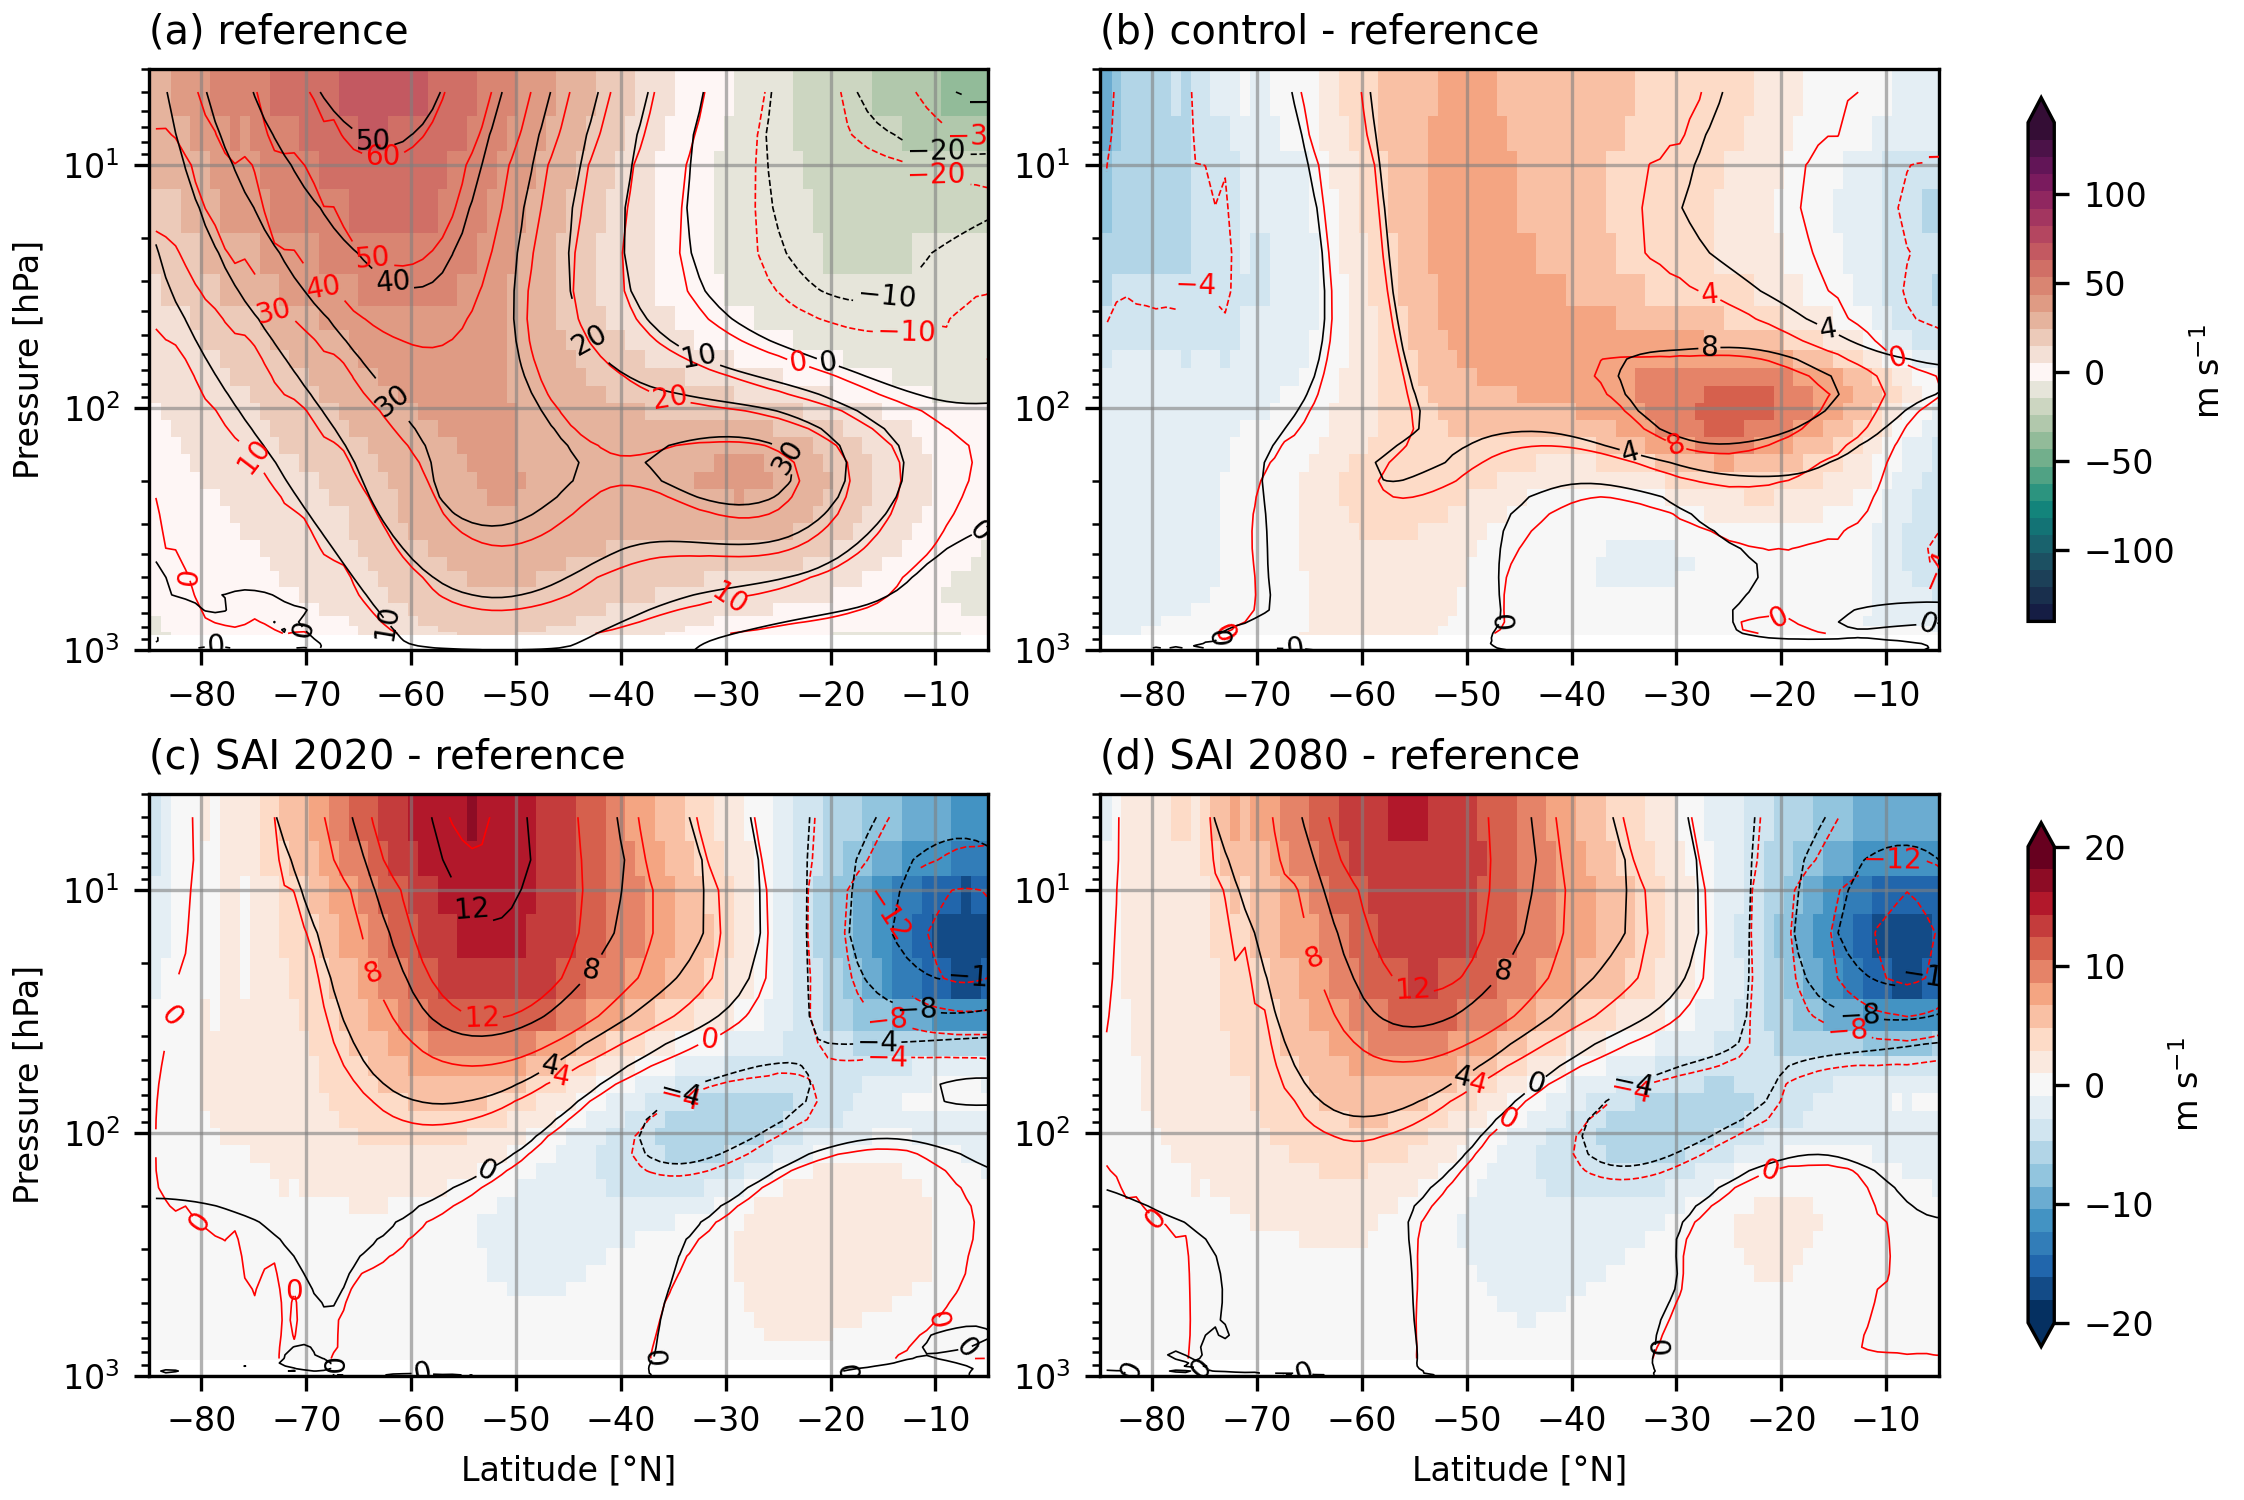
\includegraphics[width=0.95\linewidth]{images/UT_U_zmdiff_ann.png}
% 	\caption{Annual mean zonal mean zonal thermal wind (shading and black contours) and zonal mean zonal wind (red contours) for (a): Reference; (b-d): Control, SAI 2020 and SAI 2080 anomaly compared to Reference.}
% 	\label{fig:th_U_zmdiff_ann}
% \end{figure}

\begin{figure}[H]
	\centering
	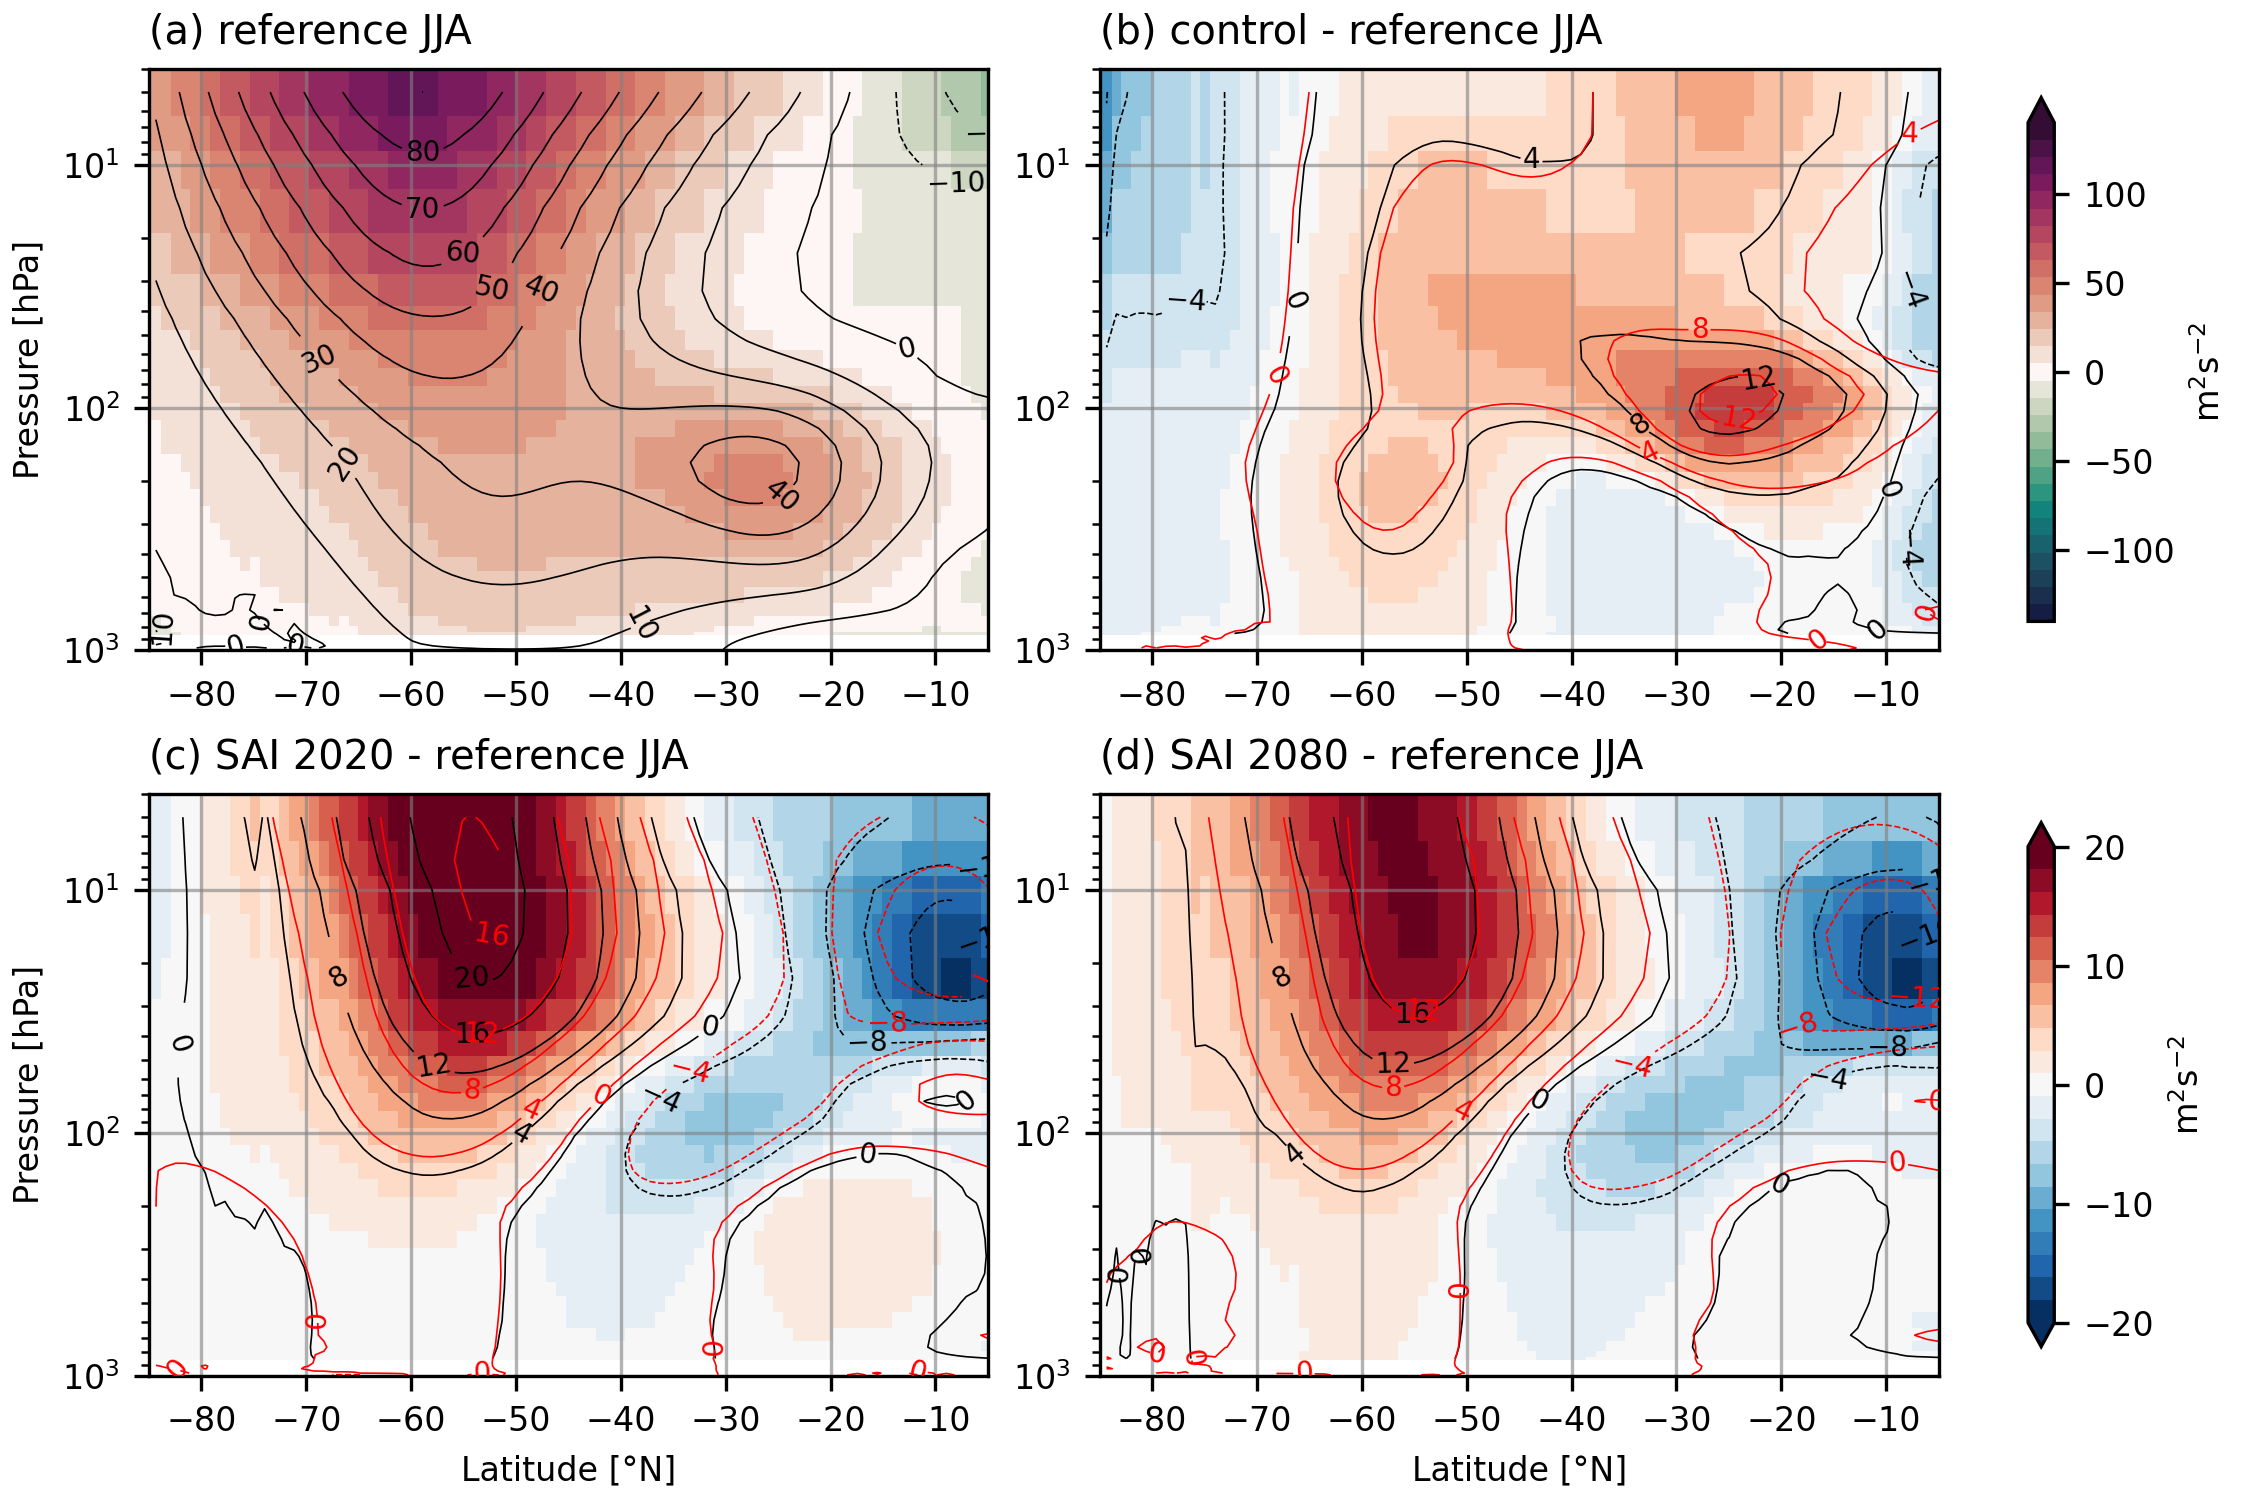
\includegraphics[width=0.95\linewidth]{images/UT_U_zmdiff_JJA.png}
	\caption{JJA mean zonal mean zonal thermal wind (shading and black contours) and zonal mean zonal wind (red contours) for (a): Reference; (b-d): Control, SAI 2020 and SAI 2080 anomaly compared to Reference.}
	\label{fig:th_U_zmdiff_JJA}
\end{figure}

% \begin{figure}[H]
% 	\centering
% 	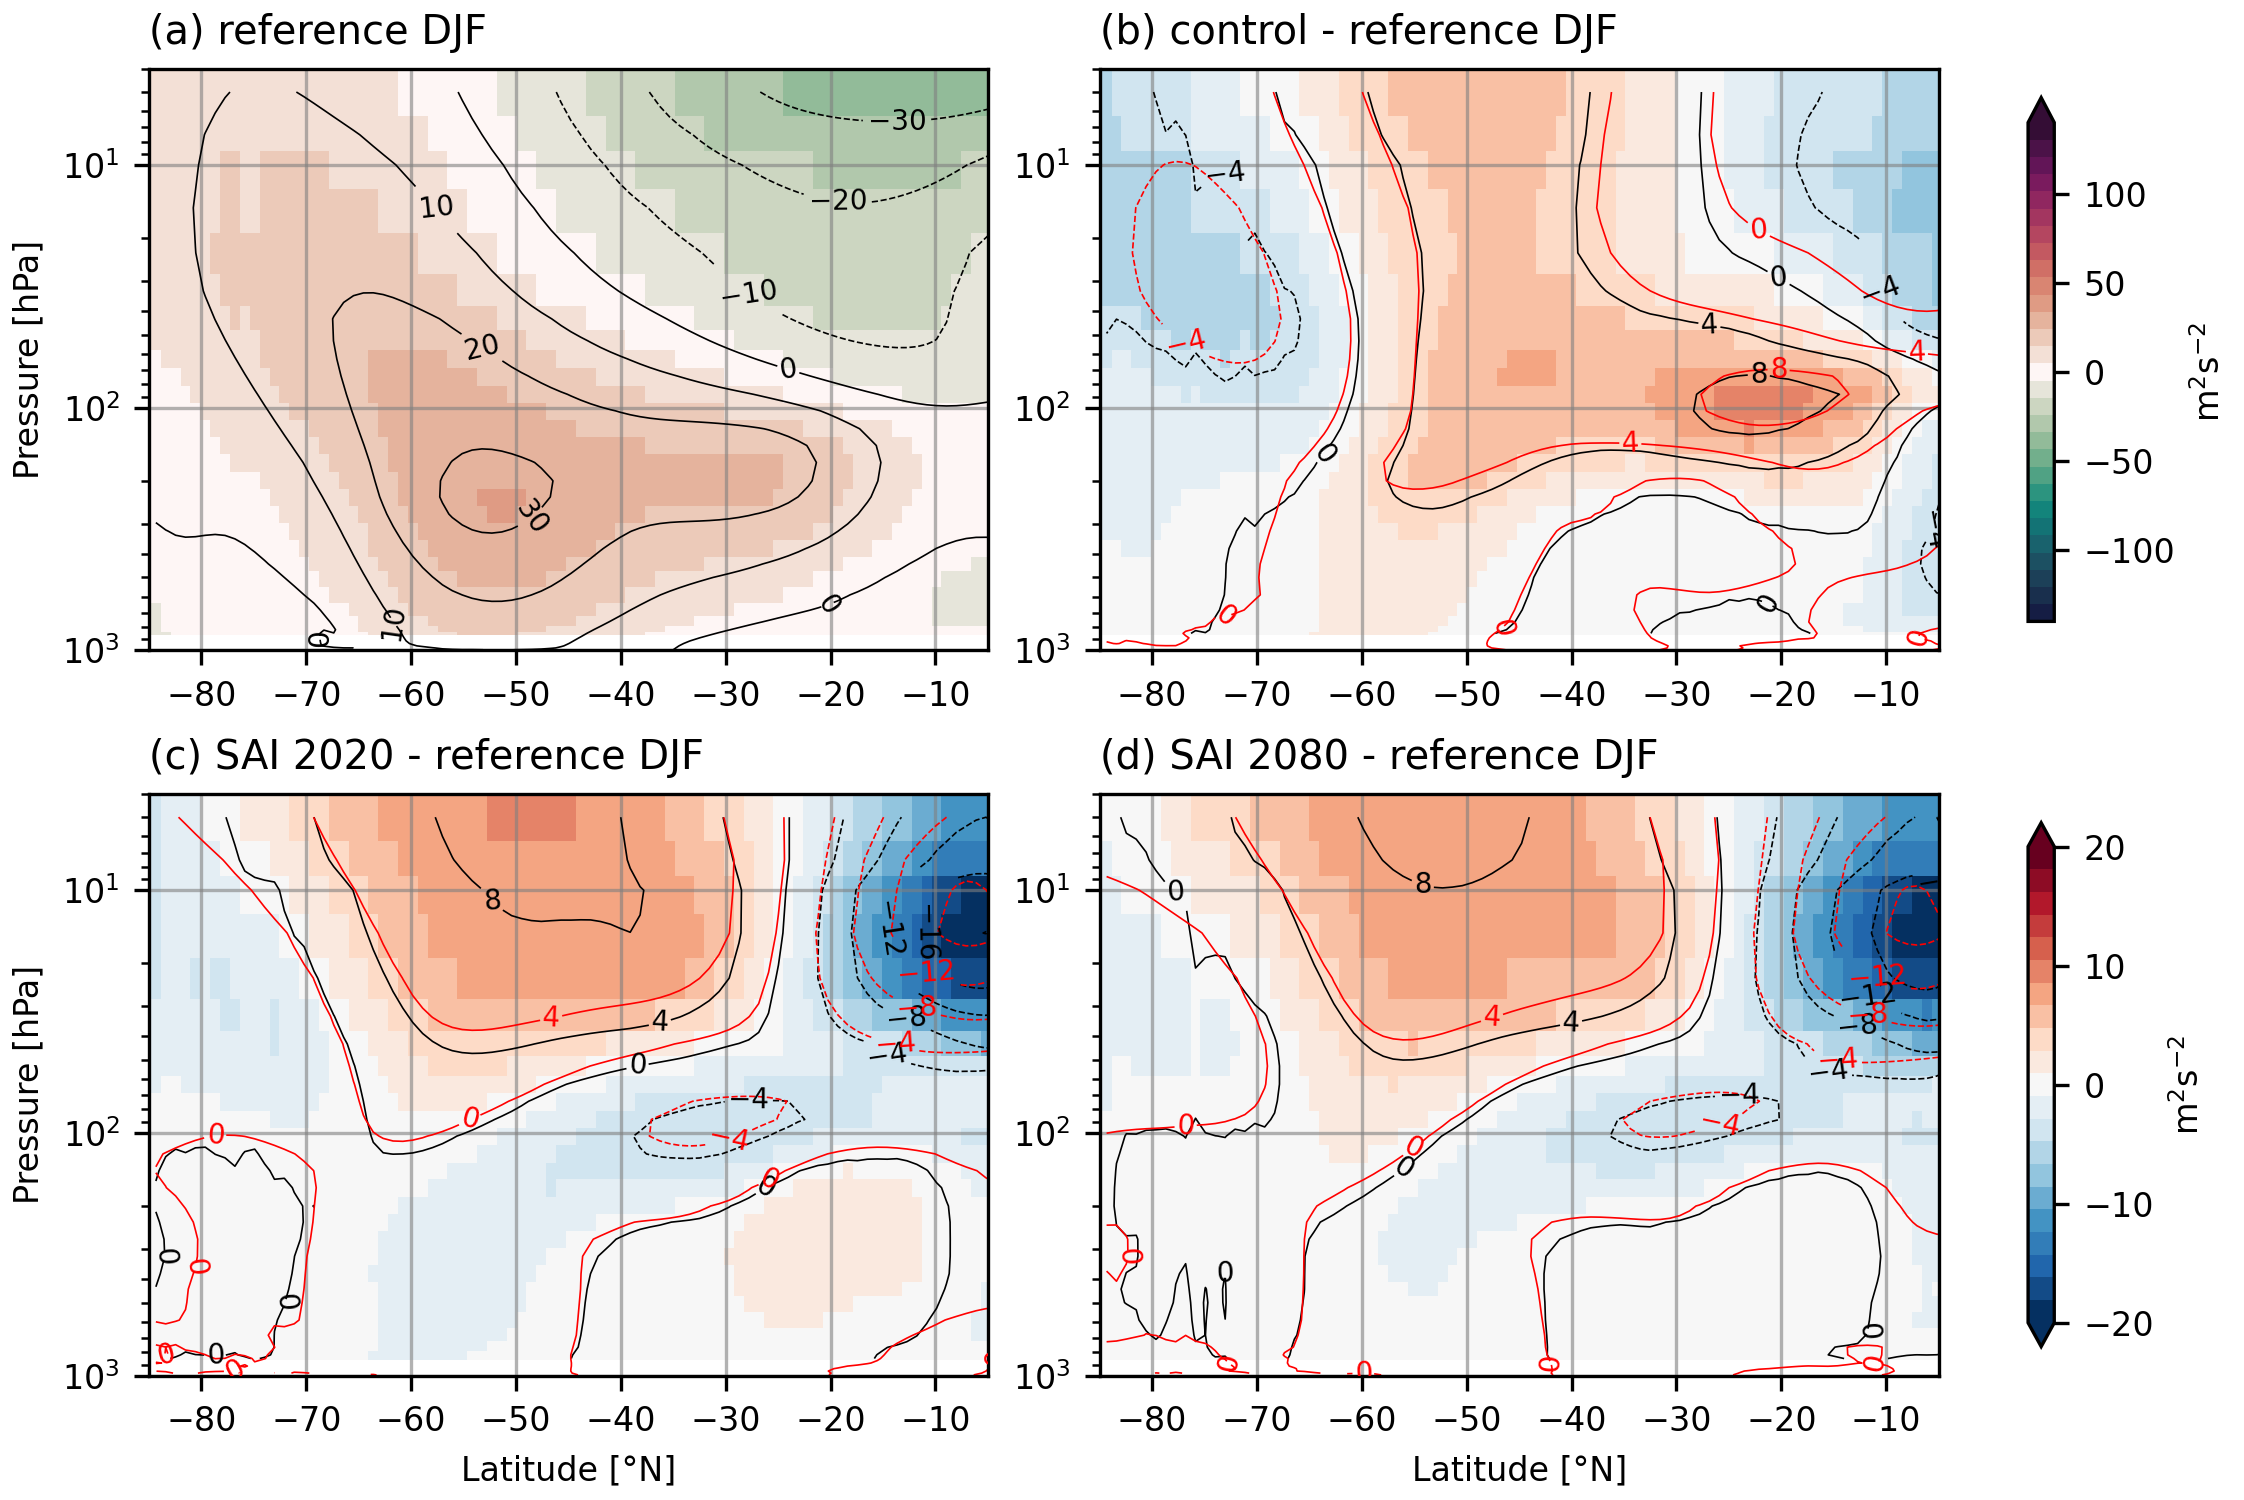
\includegraphics[width=0.95\linewidth]{images/UT_U_zmdiff_DJF.png}
% 	\caption{DJF mean zonal mean zonal thermal wind (shading and black contours) and zonal mean zonal wind (red contours) for (a): Reference; (b-d): Control, SAI 2020 and SAI 2080 anomaly compared to Reference.}
% 	\label{fig:th_U_zmdiff_DJF}
% \end{figure}

\begin{figure}[H]
	\centering
	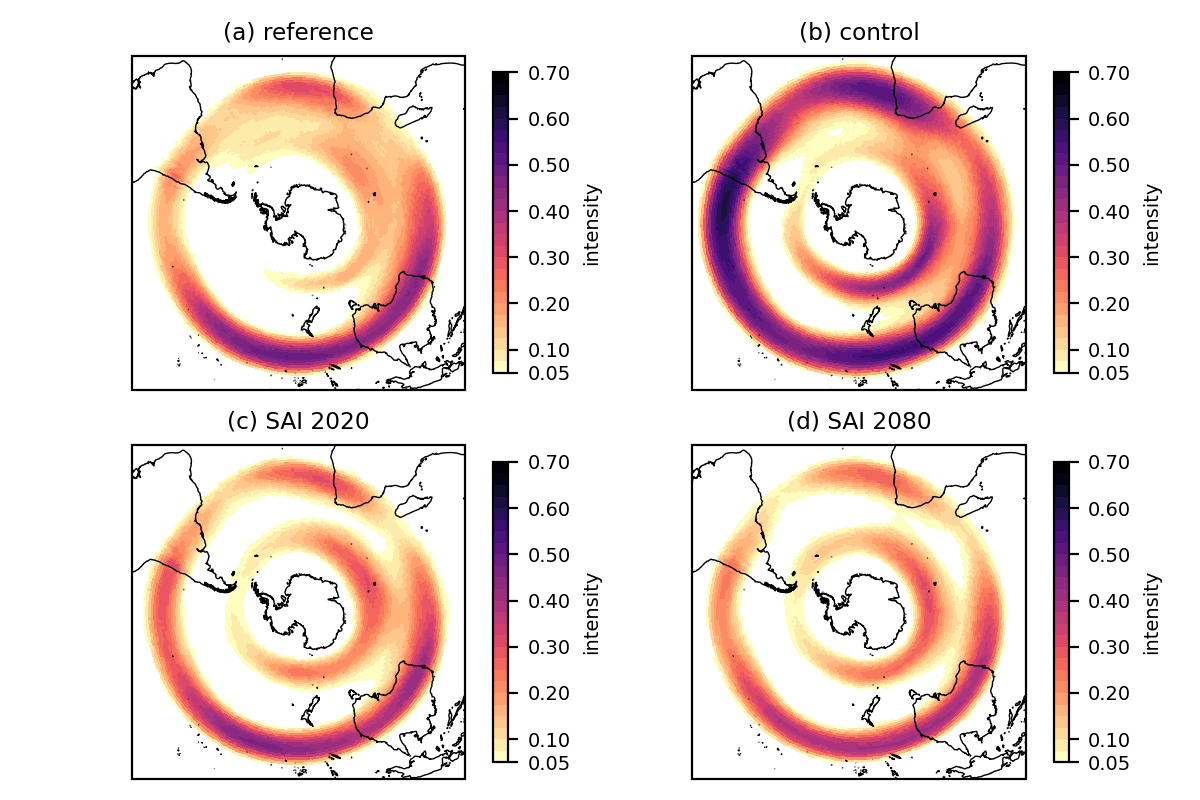
\includegraphics[width=0.95\linewidth]{images/STJ_map_JJA.png}
	\caption{JJA subtropical jet intensity map for (a) Reference, (b) Control, (c) SAI 2020 and (d) SAI 2080.}
	\label{fig:STJ_map_JJA}
\end{figure}


\subsection{Eddy-driven Jet}
More poleward, around 50°S, another jet structure appears, mostly visible in Figure \ref{fig:STJ_map_JJA}. The zonal wind in this area increases, most notably in Control, which is also visible in Figure \ref{fig:th_U_zmdiff_JJA}. Beacuse this jet is driven by eddy activity, the zonal mean eddy kinetic energy (EKE) and EKE anomalies are shown in Figure \ref{fig:EKE_U_zmdiff_JJA}.

Around 50°S and 300 hPa, there is a peak in EKE, i.e. high eddy activity. In Control the EKE decreases on the lower equatorward side of the jet and increases on the upper poleward side, indicating that the jet shifts poleward and upward. In SAI 2020 and SAI 2080 the EKE shows small changes relative to Control, with the most notable change the decrease around 45°S, right in between the EDJ and the STJ. 

The eddy-driven jet intensity map in Figure \ref{fig:EDJ_map_JJA} is also shown to increase in intensity in Control and slightly decrease in both SAI 2020 and SAI 2080. The spatial pattern remains largely unchanged in all scenarios. 

\begin{figure}[H]
	\centering
	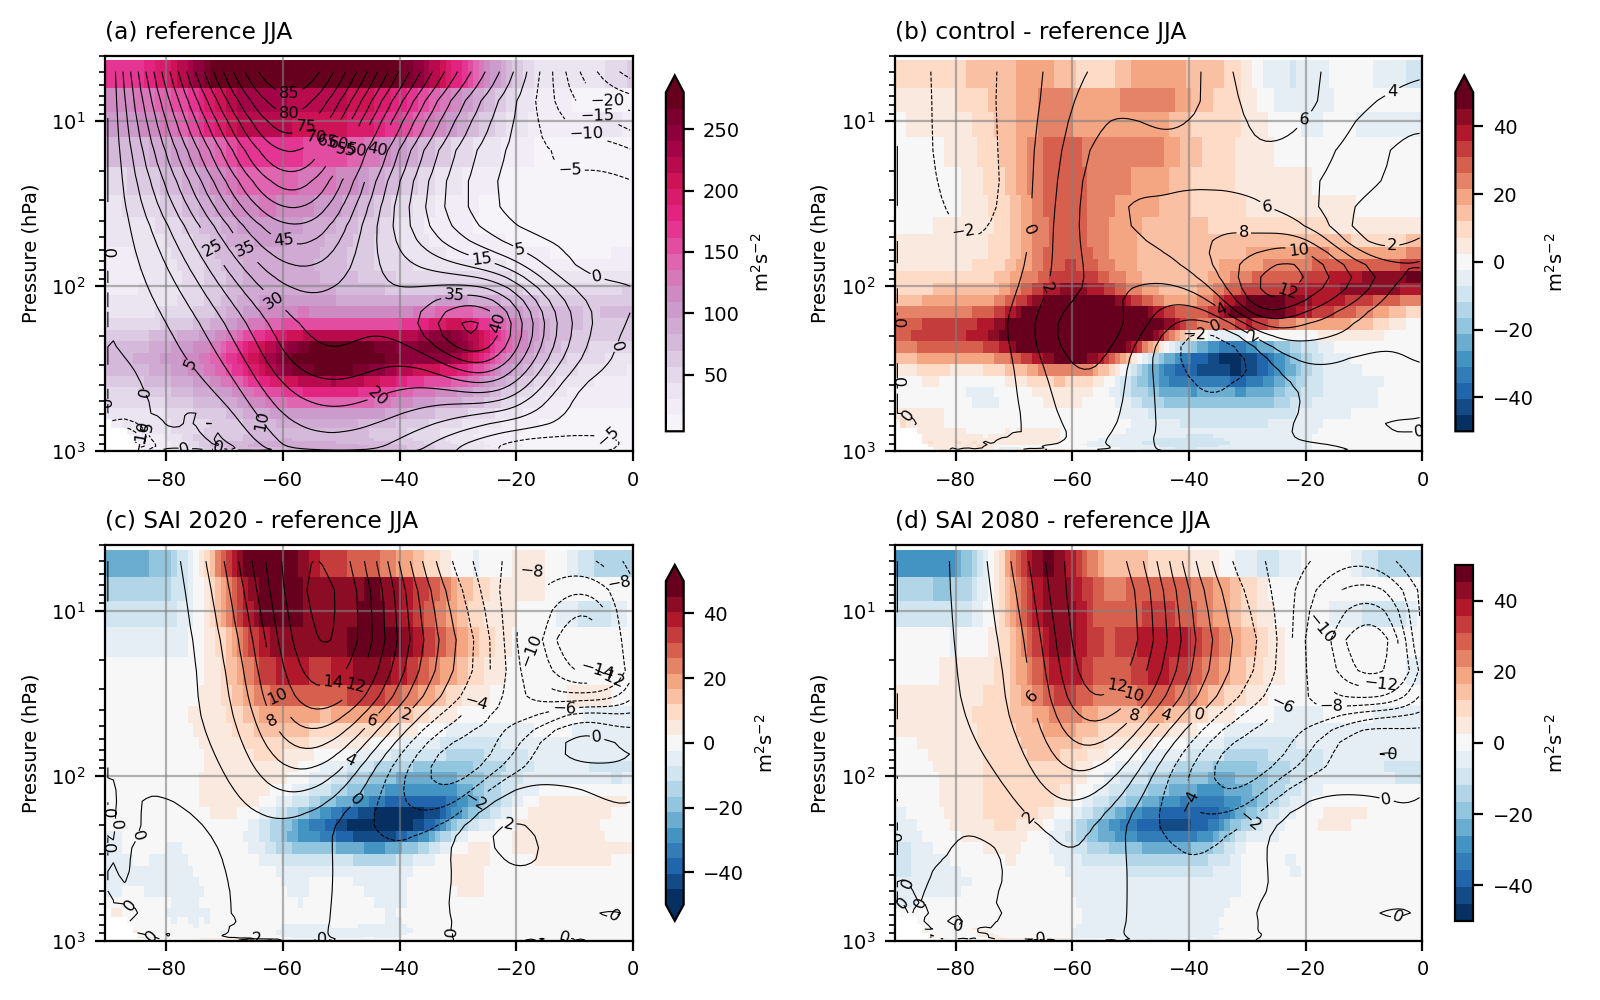
\includegraphics[width=0.95\linewidth]{images/EKE_U_zmdiff_JJA.png}
	\caption{JJA mean zonal mean eddy kinetic energy (shading) and zonal mean zonal wind (contours) for (a): Reference; (b-d): Control, SAI 2020 and SAI 2080 anomaly compared to Reference.}
	\label{fig:EKE_U_zmdiff_JJA}
\end{figure}

\begin{figure}[H]
	\centering
	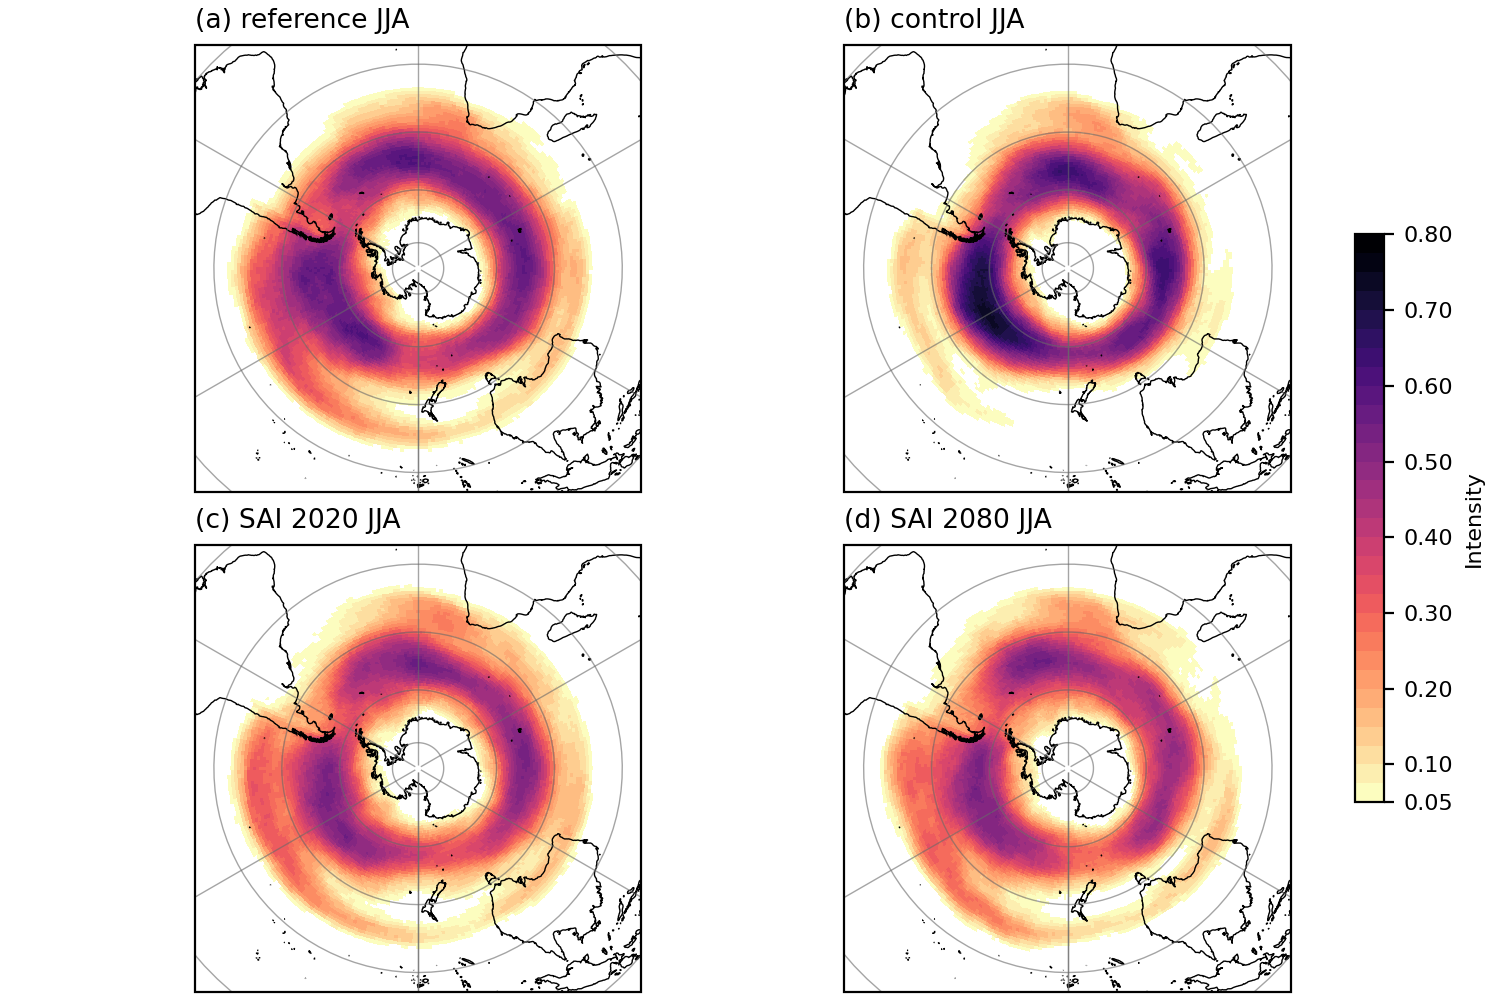
\includegraphics[width=0.95\linewidth]{images/EDJ_map_JJA.png}
	\caption{JJA eddy-driven jet intensity map for (a) Reference, (b) Control, (c) SAI 2020 and (d) SAI 2080.}
	\label{fig:EDJ_map_JJA}
\end{figure}

There is a clear correlation between the EKE anomalies and zonal mean zonal wind anomalies, thus we look at the kinetic energy to disentangle the change in zonal wind from the change in EKE. In Figure \ref{fig:KE_U_zmdiff_JJA} the zonal mean kinetic energy and zonal mean zonal wind are shown. 

For Control the increase in KE energy follows the zonal wind patterns in sign, but not in magnitude. The KE increases with the increasing zonal wind accordingly in the upper regions of the STJ, but the KE increases and decreases more in the EDJ area than would be expedted from the increase in zonal wind. 

For SAI 2020 and SAI 2080 the KE anomaly does follow the zonal wind anomaly proportionally and comparison with Figure \ref{fig:EKE_U_zmdiff_JJA} shows that the decrease in EKE is correlated with the decrease in zonal wind. This correlation is also clear when comparing the jet intensity maps in Figures \ref{fig:SJT_map_JJA} and \ref{fig:EDJ_map_JJA}.

\begin{figure}[H]
	\centering
	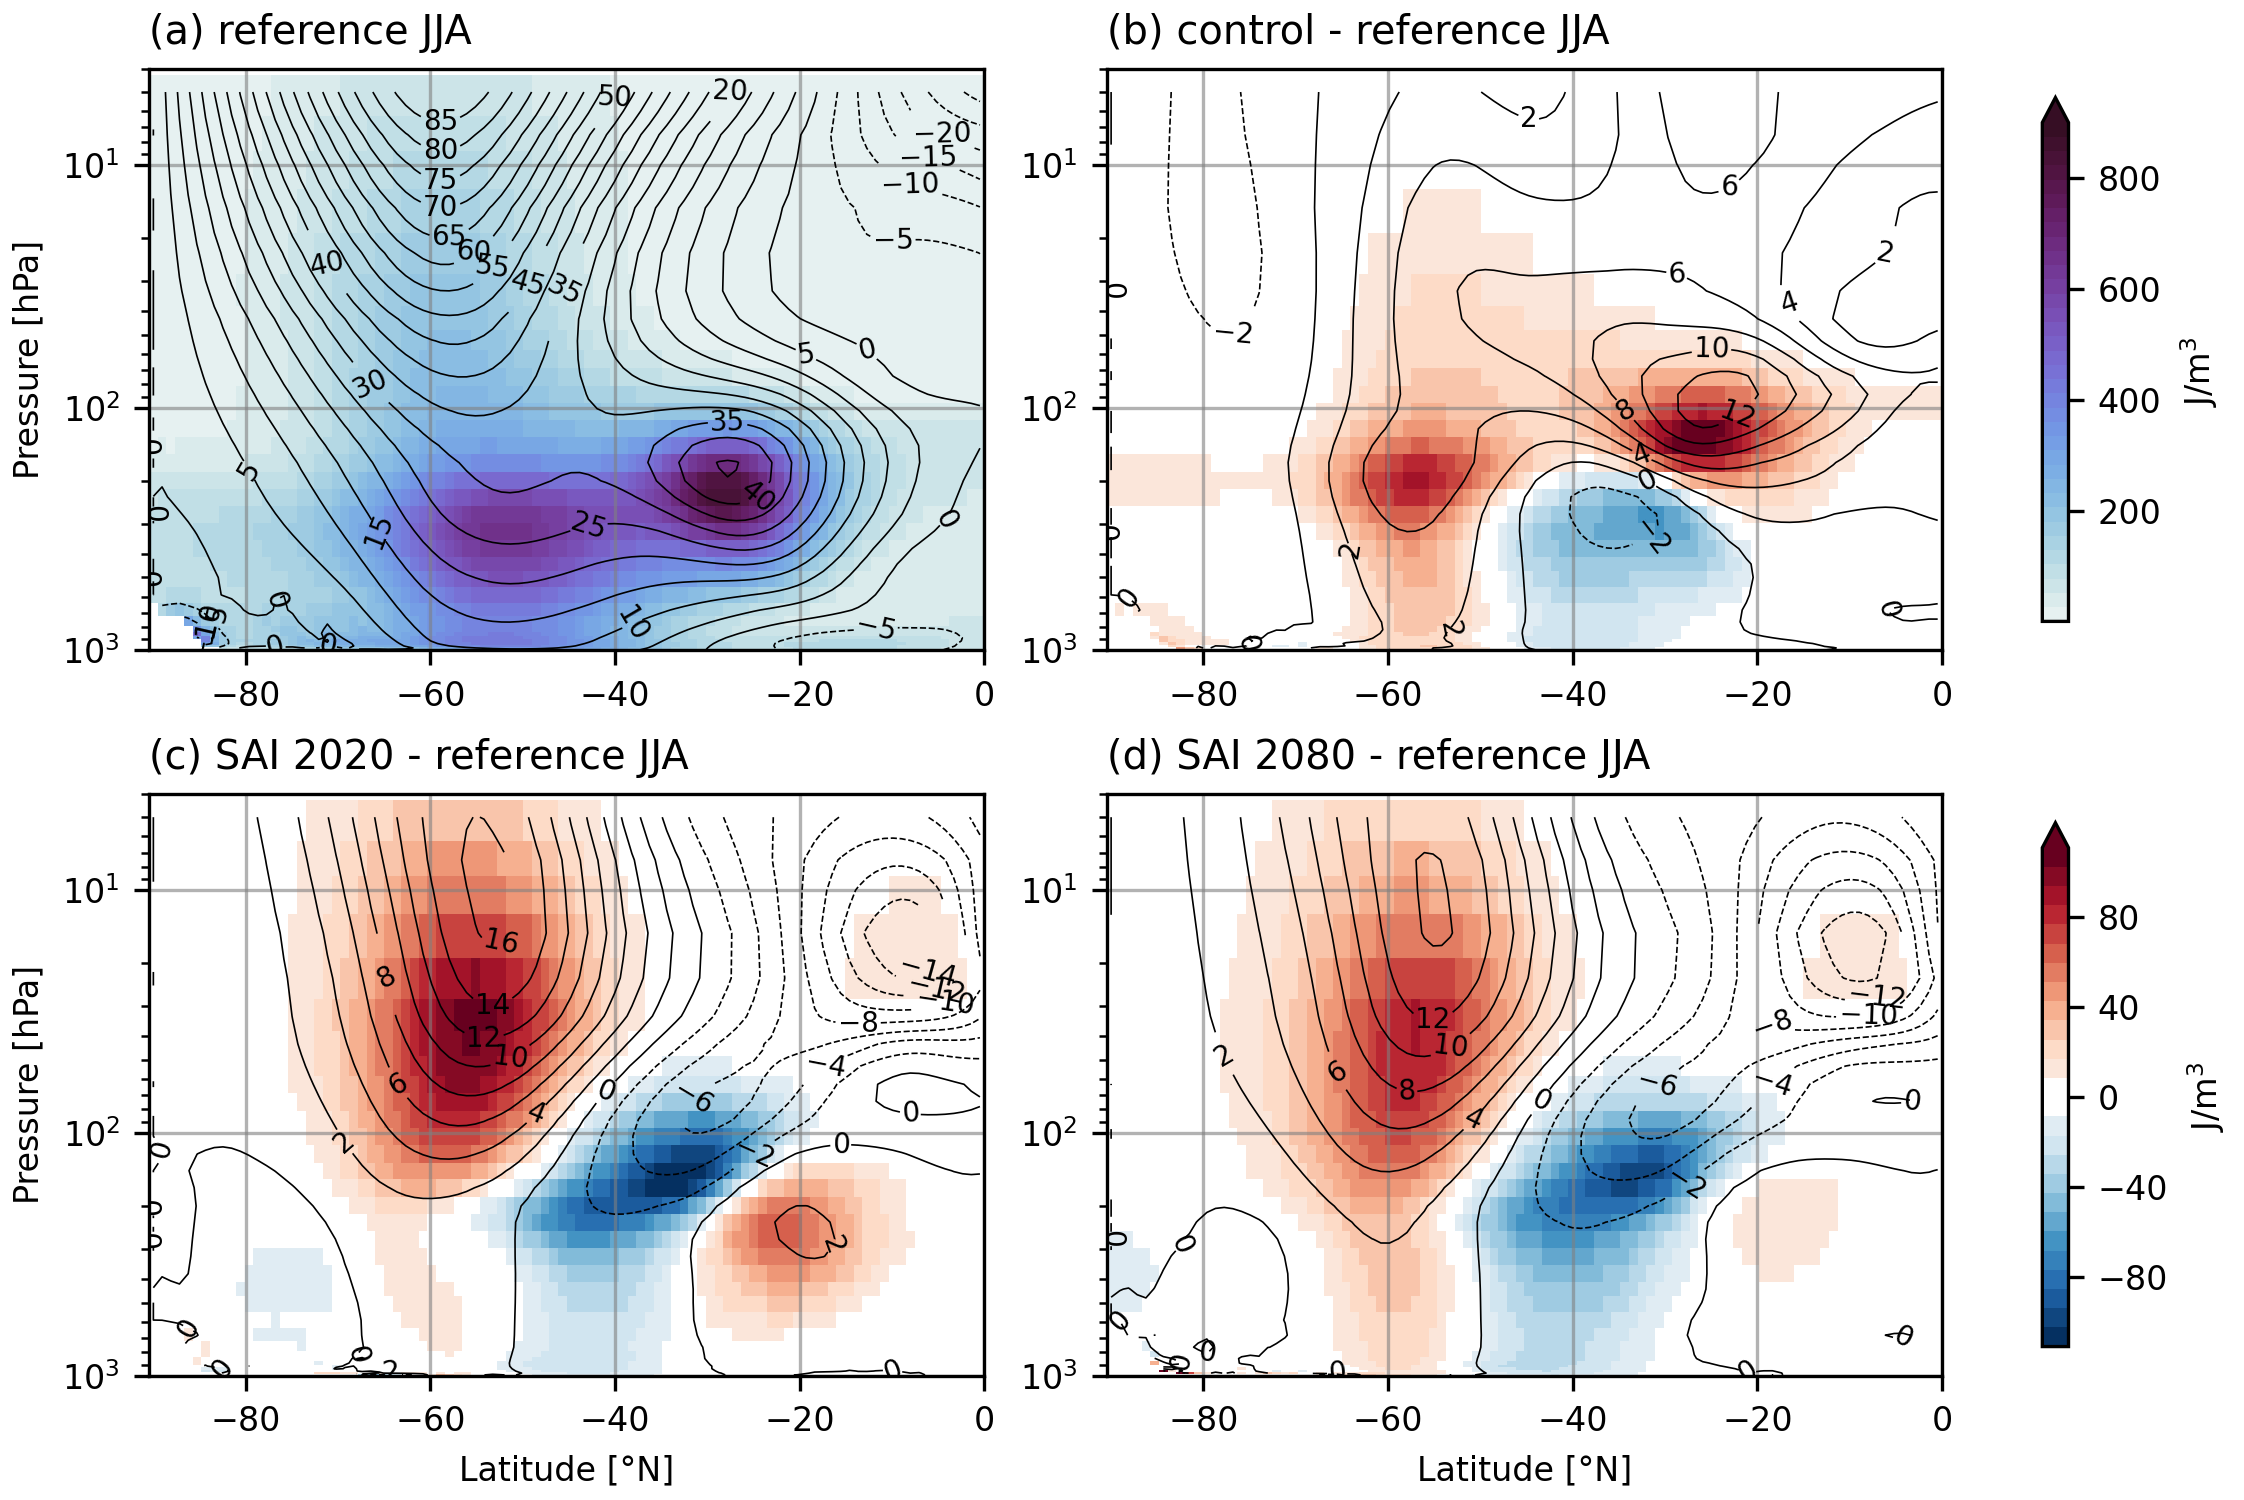
\includegraphics[width=0.95\linewidth]{images/KE_U_zmdiff_JJA.png}
	\caption{JJA mean zonal mean kinetic energy (shading) and zonal mean zonal wind (contours) for (a): Reference; (b-d): Control, SAI 2020 and SAI 2080 anomaly compared to Reference.}
	\label{fig:KE_U_zmdiff_JJA}
\end{figure}
\newpage

\section{Results Part II: Upper Stratosphere}\label{upperstrat}
This section contains the results for the SSP5-8.5, the gradual SAI and the rapid cooling SAI experiments that are relevant for analysis of the upper stratosphere and the polar night jet (PNJ).

The potential temperature and zonal wind anomalies from section \ref{lowerstrat} showed the largest differences in the JJA mean, but the polar night jet is strongest in late winter and early spring. Al figures in this section will therefore consider the August-September-October (ASO) mean. 

\subsection{Polar Night Jet}
Figure \ref{fig:PNJ_UT_U_zmdiff} shows the zonal component of the thermal wind and the anomalies in Control, SAI 2020 and SAI 2080 in ASO. As in section \ref{lowerstrat} the observed wind and the thermal wind show the same patterns, with the thermal wind consistently higher than the observed wind due to friction effects. 

In control the PNJ shifts equatorward, with its strength not significantly changing. In SAI 2020 and SAI 2080 the PNJ shifts equatorward as well, but in contrast to Control the wind speed increases significantly. The pattern in SAI 2080 is the same as in SAI 2020, but the increase is much smaller. 

The kinetic energy per unit mass shown in Figure \ref{fig:PNJ_KE_U_zmdiff} shows largely the same pattern as the thermal wind in Figure \ref{fig:PNJ_UT_U_zmdiff}. In Figure \ref{fig:PNJ_EKE_U_zmdiff} the eddy kinetic energy is shown. In Control there is a decrease in EKE on the poleward side of the PNJ that is large relative to the KE decrease, indicating a relative deacrease in eddy activity.

The decrease in EKE over the Antarctic is visible in SAI 2020 and SAI 2080 as well, though lower, it still indicates a relative decrease in eddy activity. Where the KE increase is largest, the EKE increases the most as well, though contrastingly there is a second peak in EKE increase more equatorward, indicating an increase in eddy activity on the equatorward side of the PNJ. As with the KE, this increase is stronger in SAI 2020 than it is in SAI 2080. 

\begin{figure}[H]
	\centering
	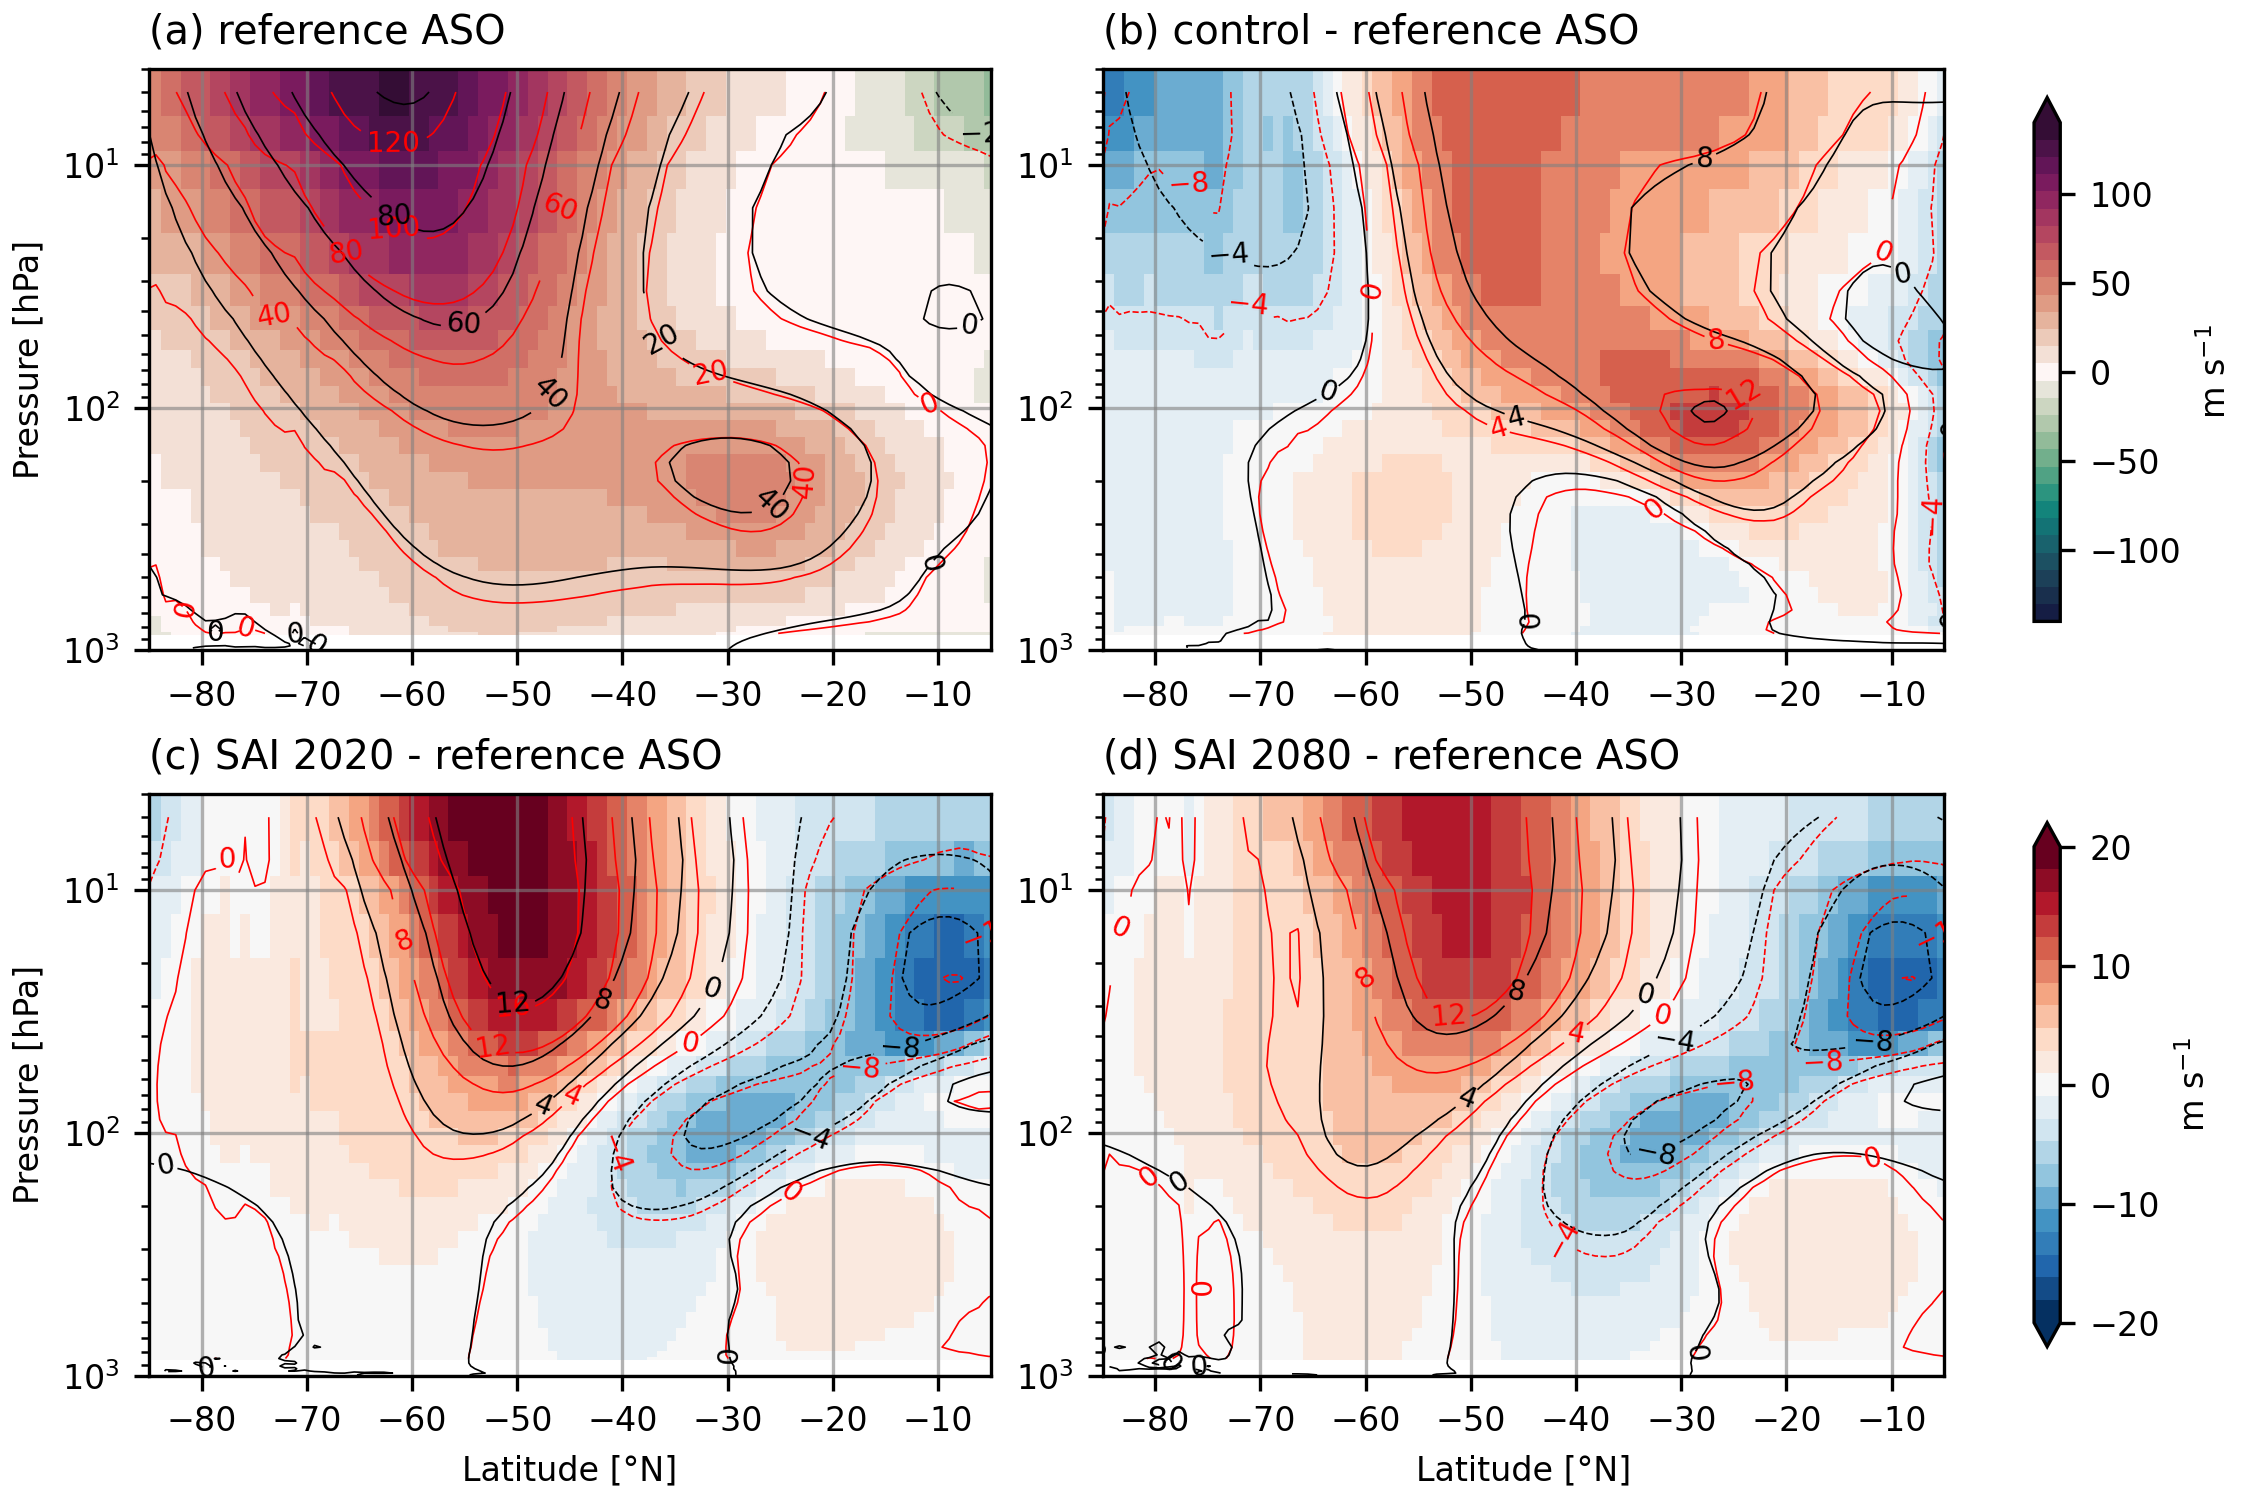
\includegraphics[width=0.95\linewidth]{images/PNJ_UT_U_zmdiff.png}
	\caption{ASO mean zonal mean kinetic energy (shading) and zonal mean zonal wind (contours) for (a): Reference; (b-d): Control, SAI 2020 and SAI 2080 anomaly compared to Reference.}
	\label{fig:PNJ_UT_U_zmdiff}
\end{figure}

\begin{figure}[H]
	\centering
	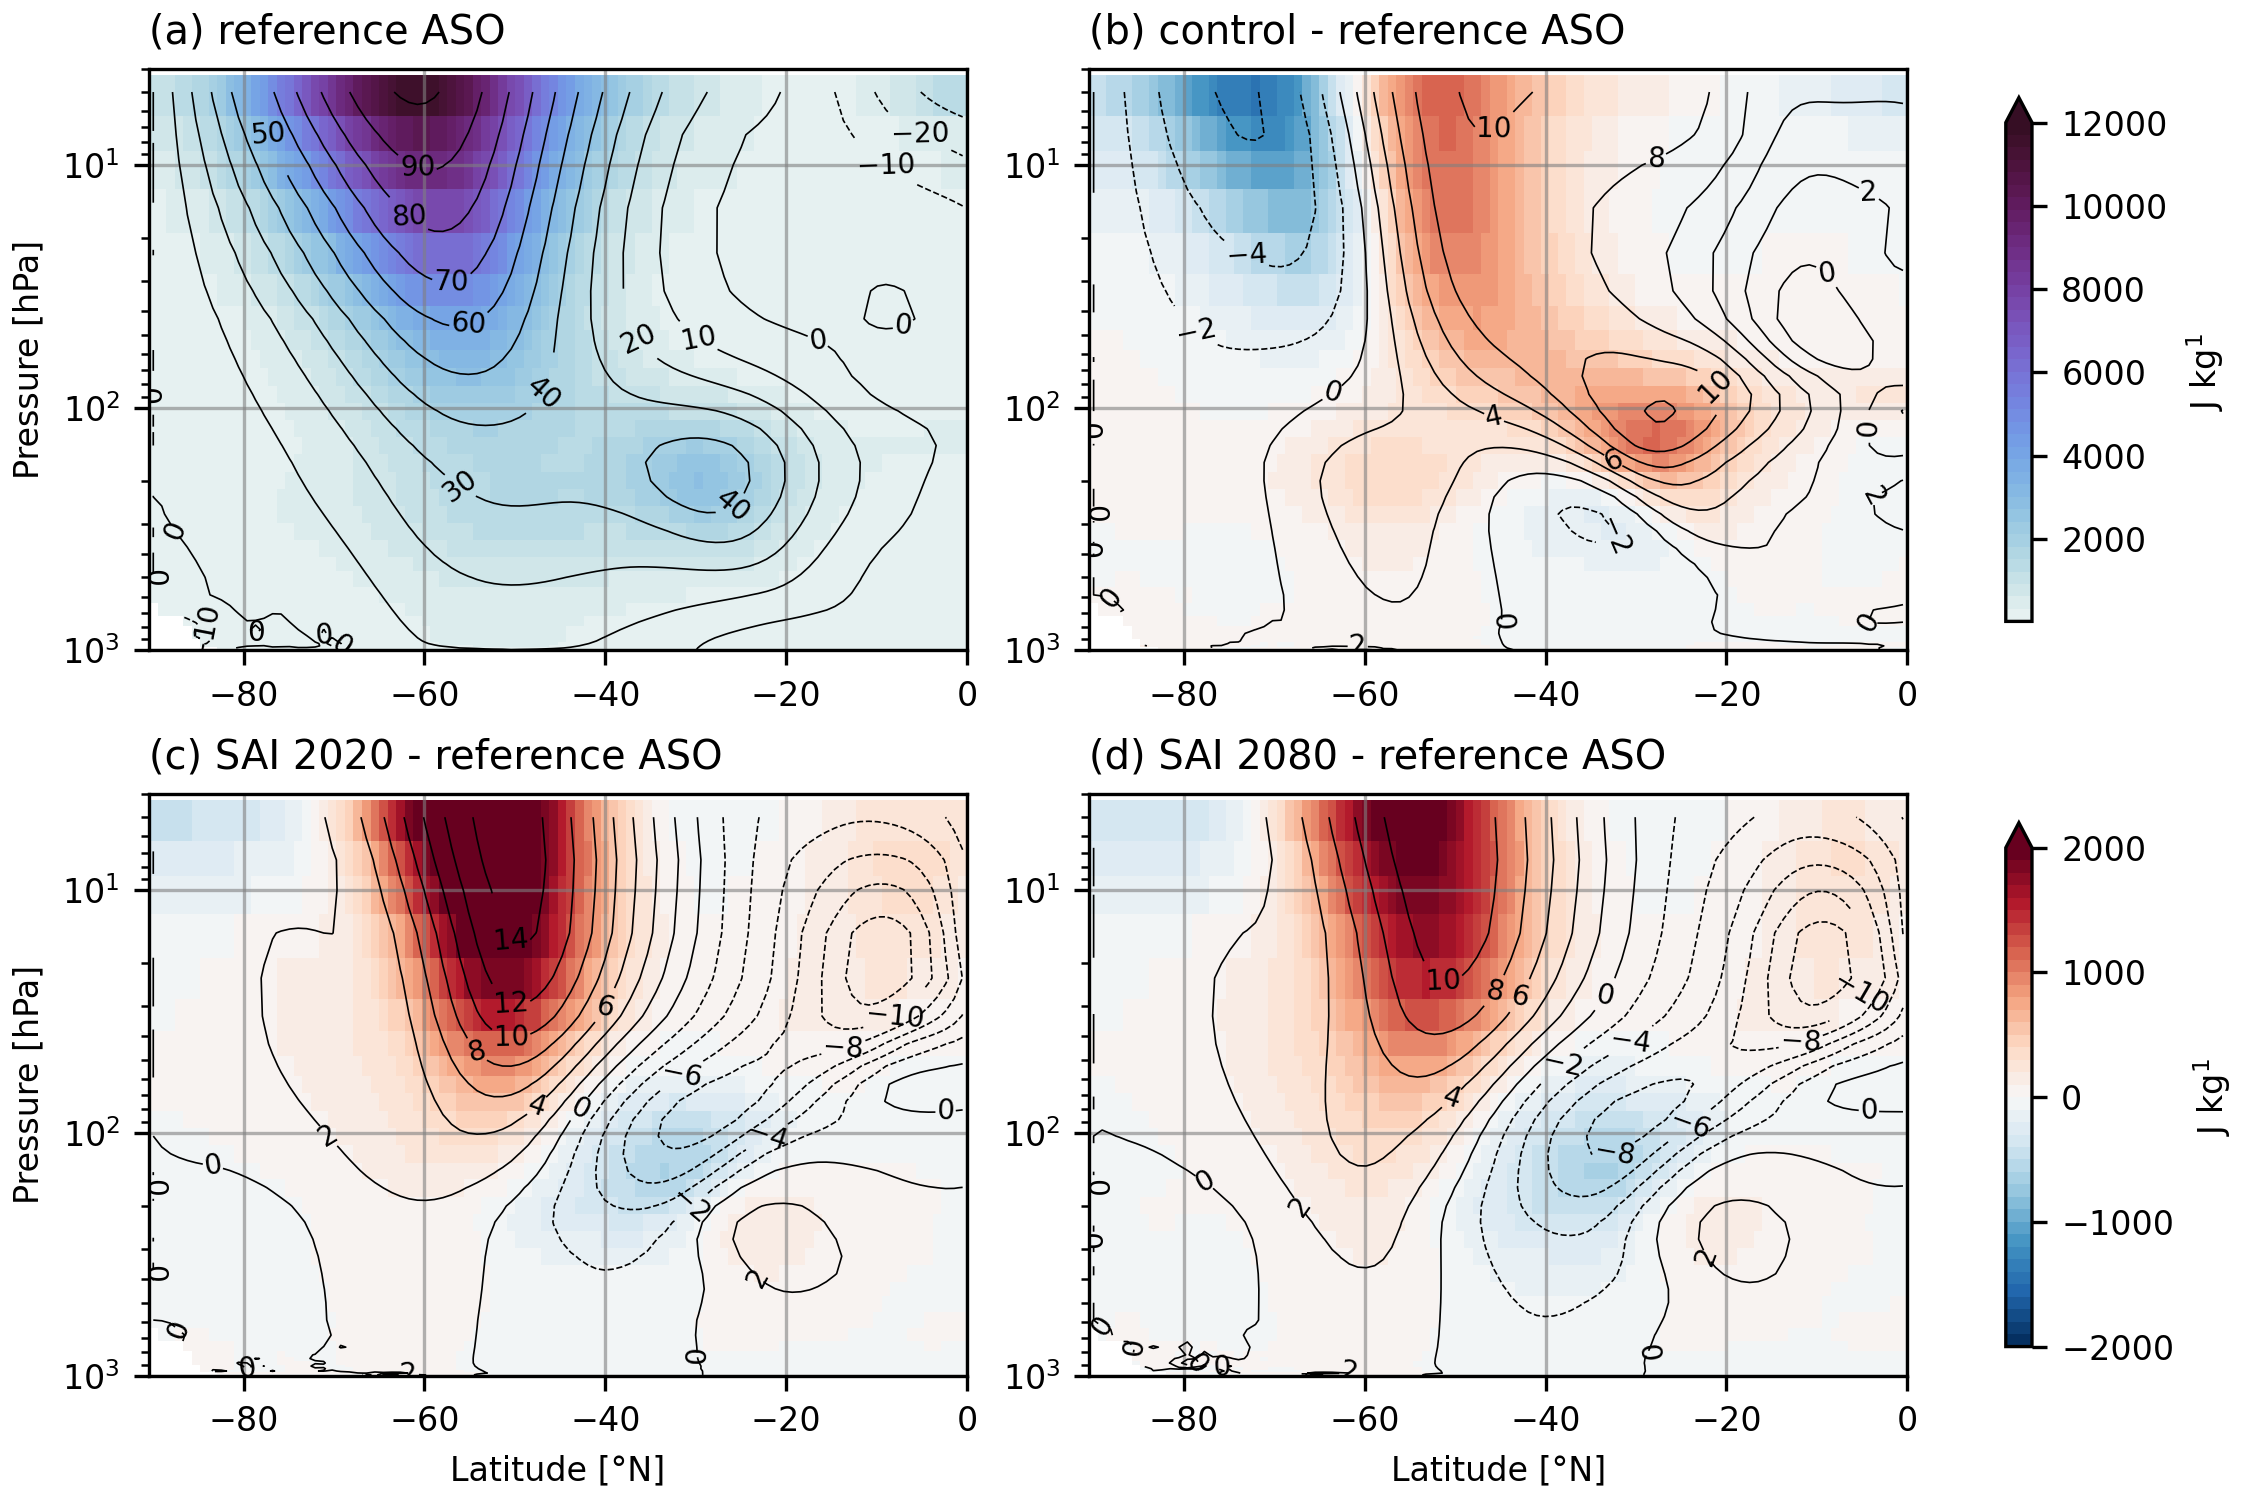
\includegraphics[width=0.95\linewidth]{images/PNJ_KE_U_zmdiff.png}
	\caption{JJA mean zonal mean eddy kinetic energy (shading) and zonal mean zonal wind (contours) for (a): Reference; (b-d): Control, SAI 2020 and SAI 2080 anomaly compared to Reference.}
	\label{fig:PNJ_KE_U_zmdiff}
\end{figure}


\begin{figure}[H]
	\centering
	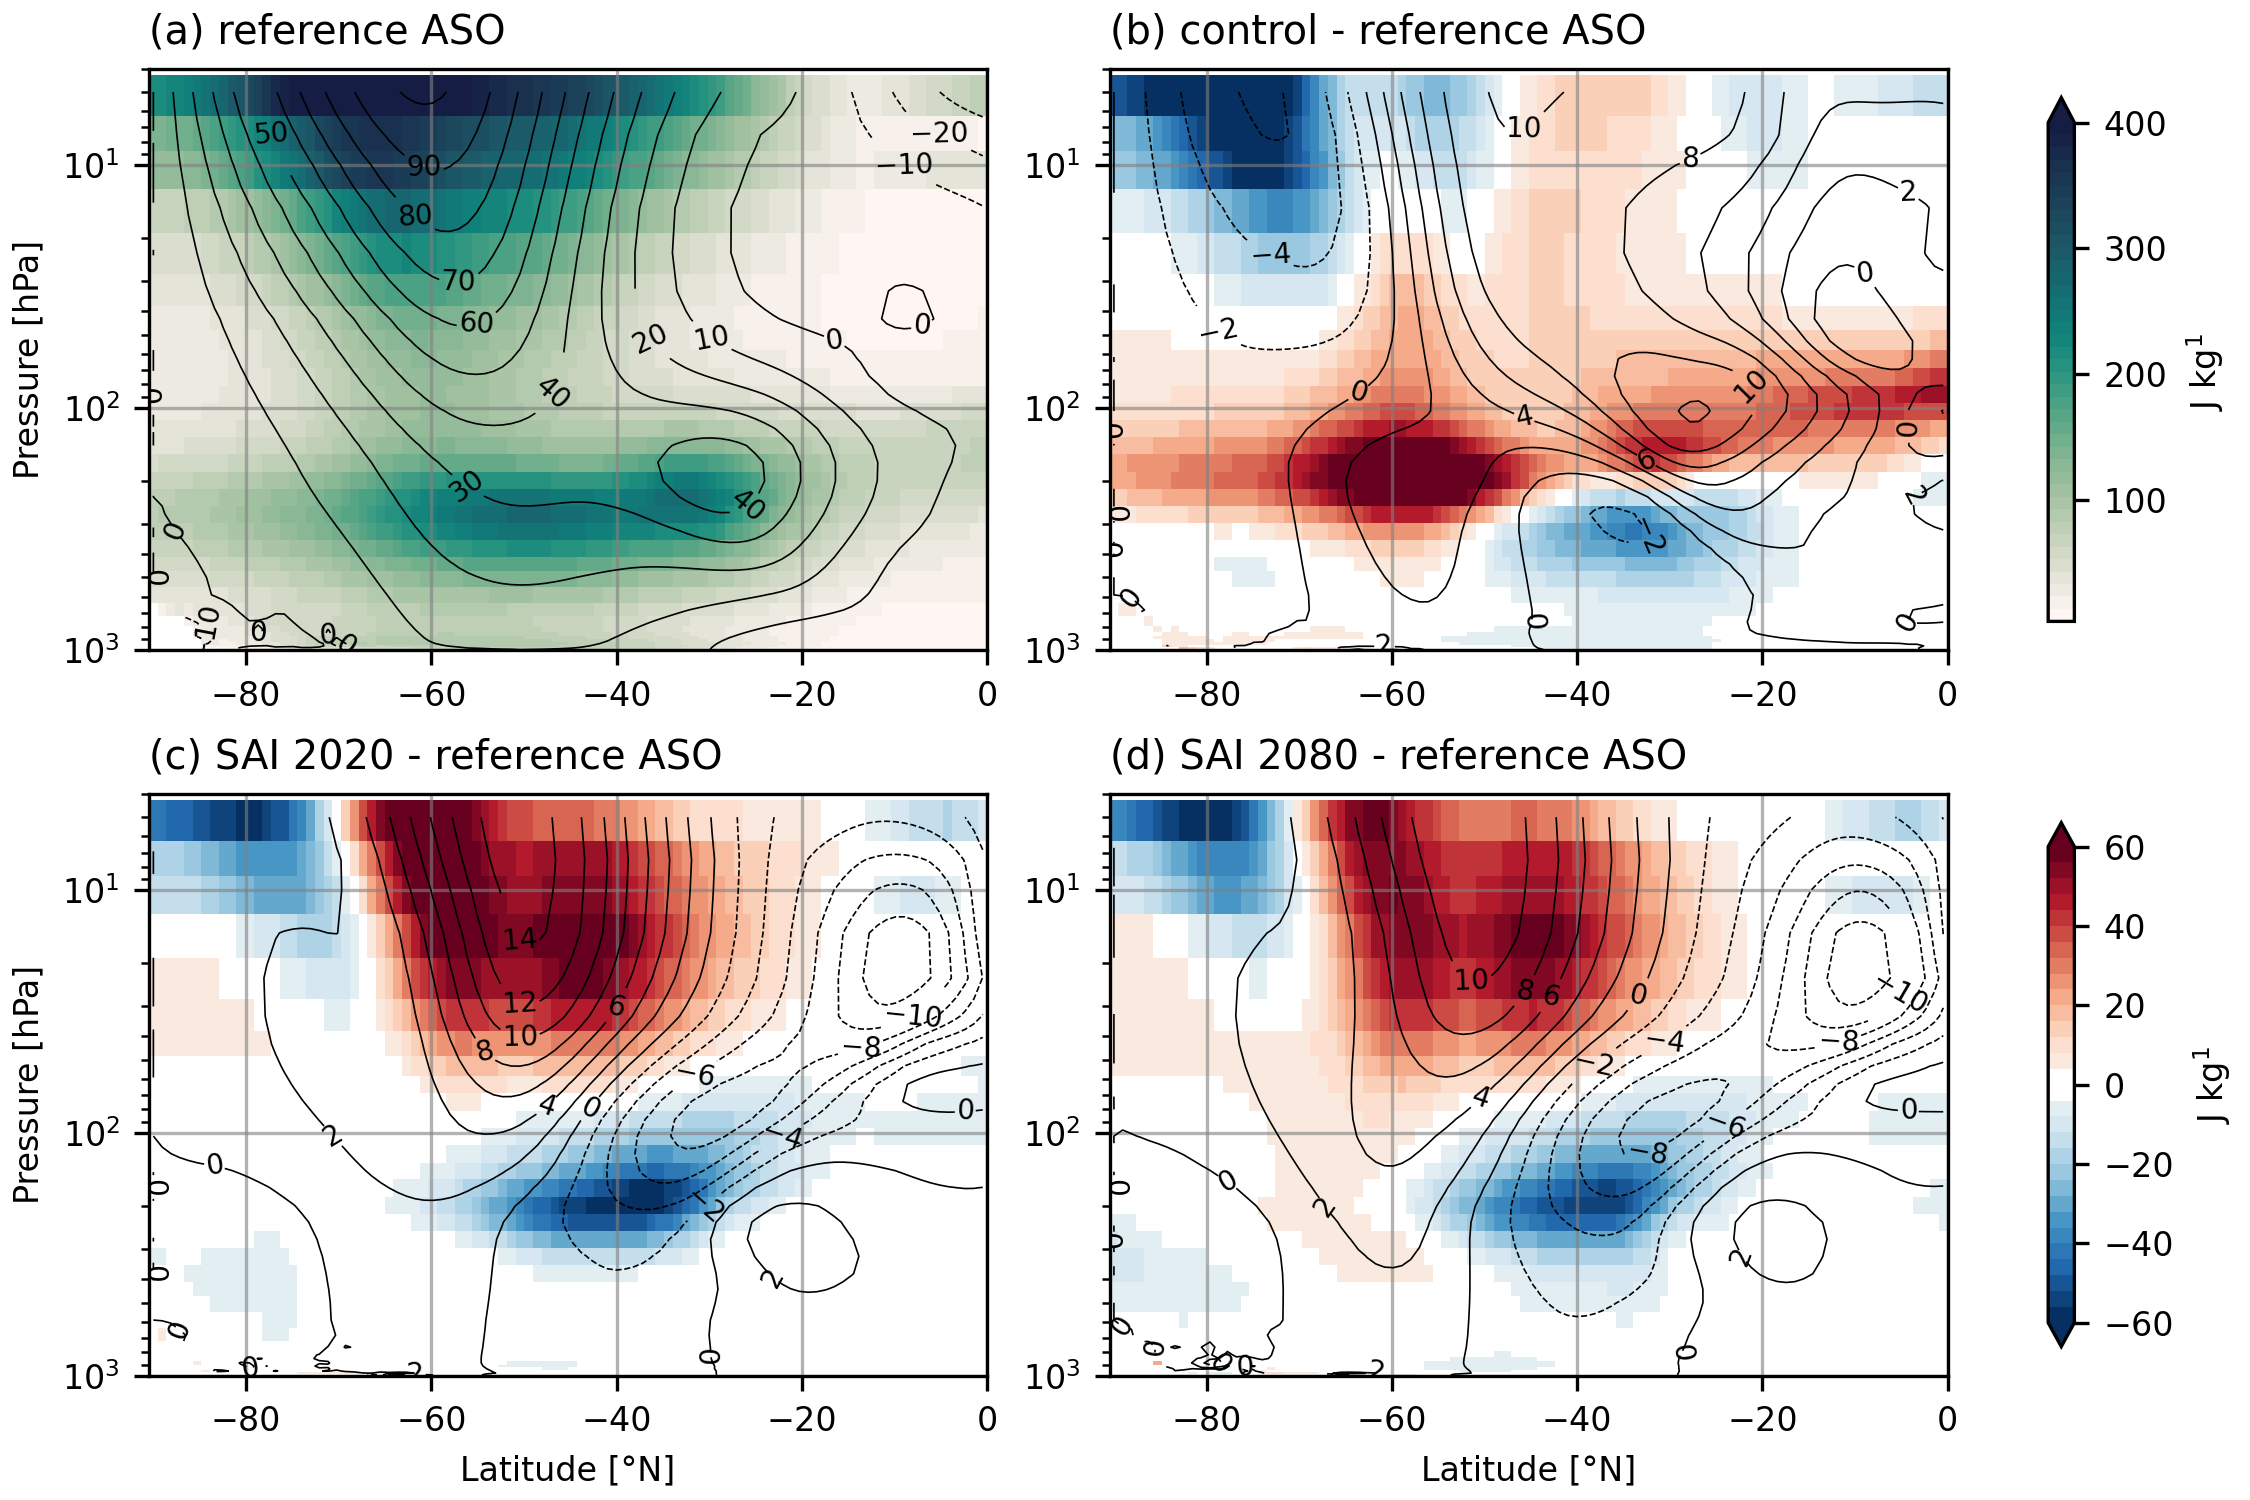
\includegraphics[width=0.95\linewidth]{images/PNJ_EKE_U_zmdiff.png}
	\caption{JJA mean zonal mean eddy kinetic energy (shading) and zonal mean zonal wind (contours) for (a): Reference; (b-d): Control, SAI 2020 and SAI 2080 anomaly compared to Reference.}
	\label{fig:PNJ_EKE_U_zmdiff}
\end{figure}

The increasing strength of the PNJ is again visible in the polar night jet intensity map in Figure \ref{fig:PNJ_map}. The PNJ intensifies in all scenarios, most strongly in SAI 2020, followed by SAI 2080 and lastly Control. The same trend is observed for the position, with the PNJ shifting equatorward in all scenarios. This equatorward shift is more clearly observed in Figure \ref{fig:PNJ_maxloc}, where the mean location of the maximum observed wind speed is shown. The scenario with the largest shift varies per location, with hardly any movement in any scenario in the 0°-60°E section, Control shifting the most in the 120°-180°E section, and SAI 2020 shifting the most in the 240°-300°E section. The shift in SAI 2080 is mostly consistent with SAI 2020, but deviates in the 240°-300°E section, coinciding with Control there.

\begin{figure}[H]
	\centering
	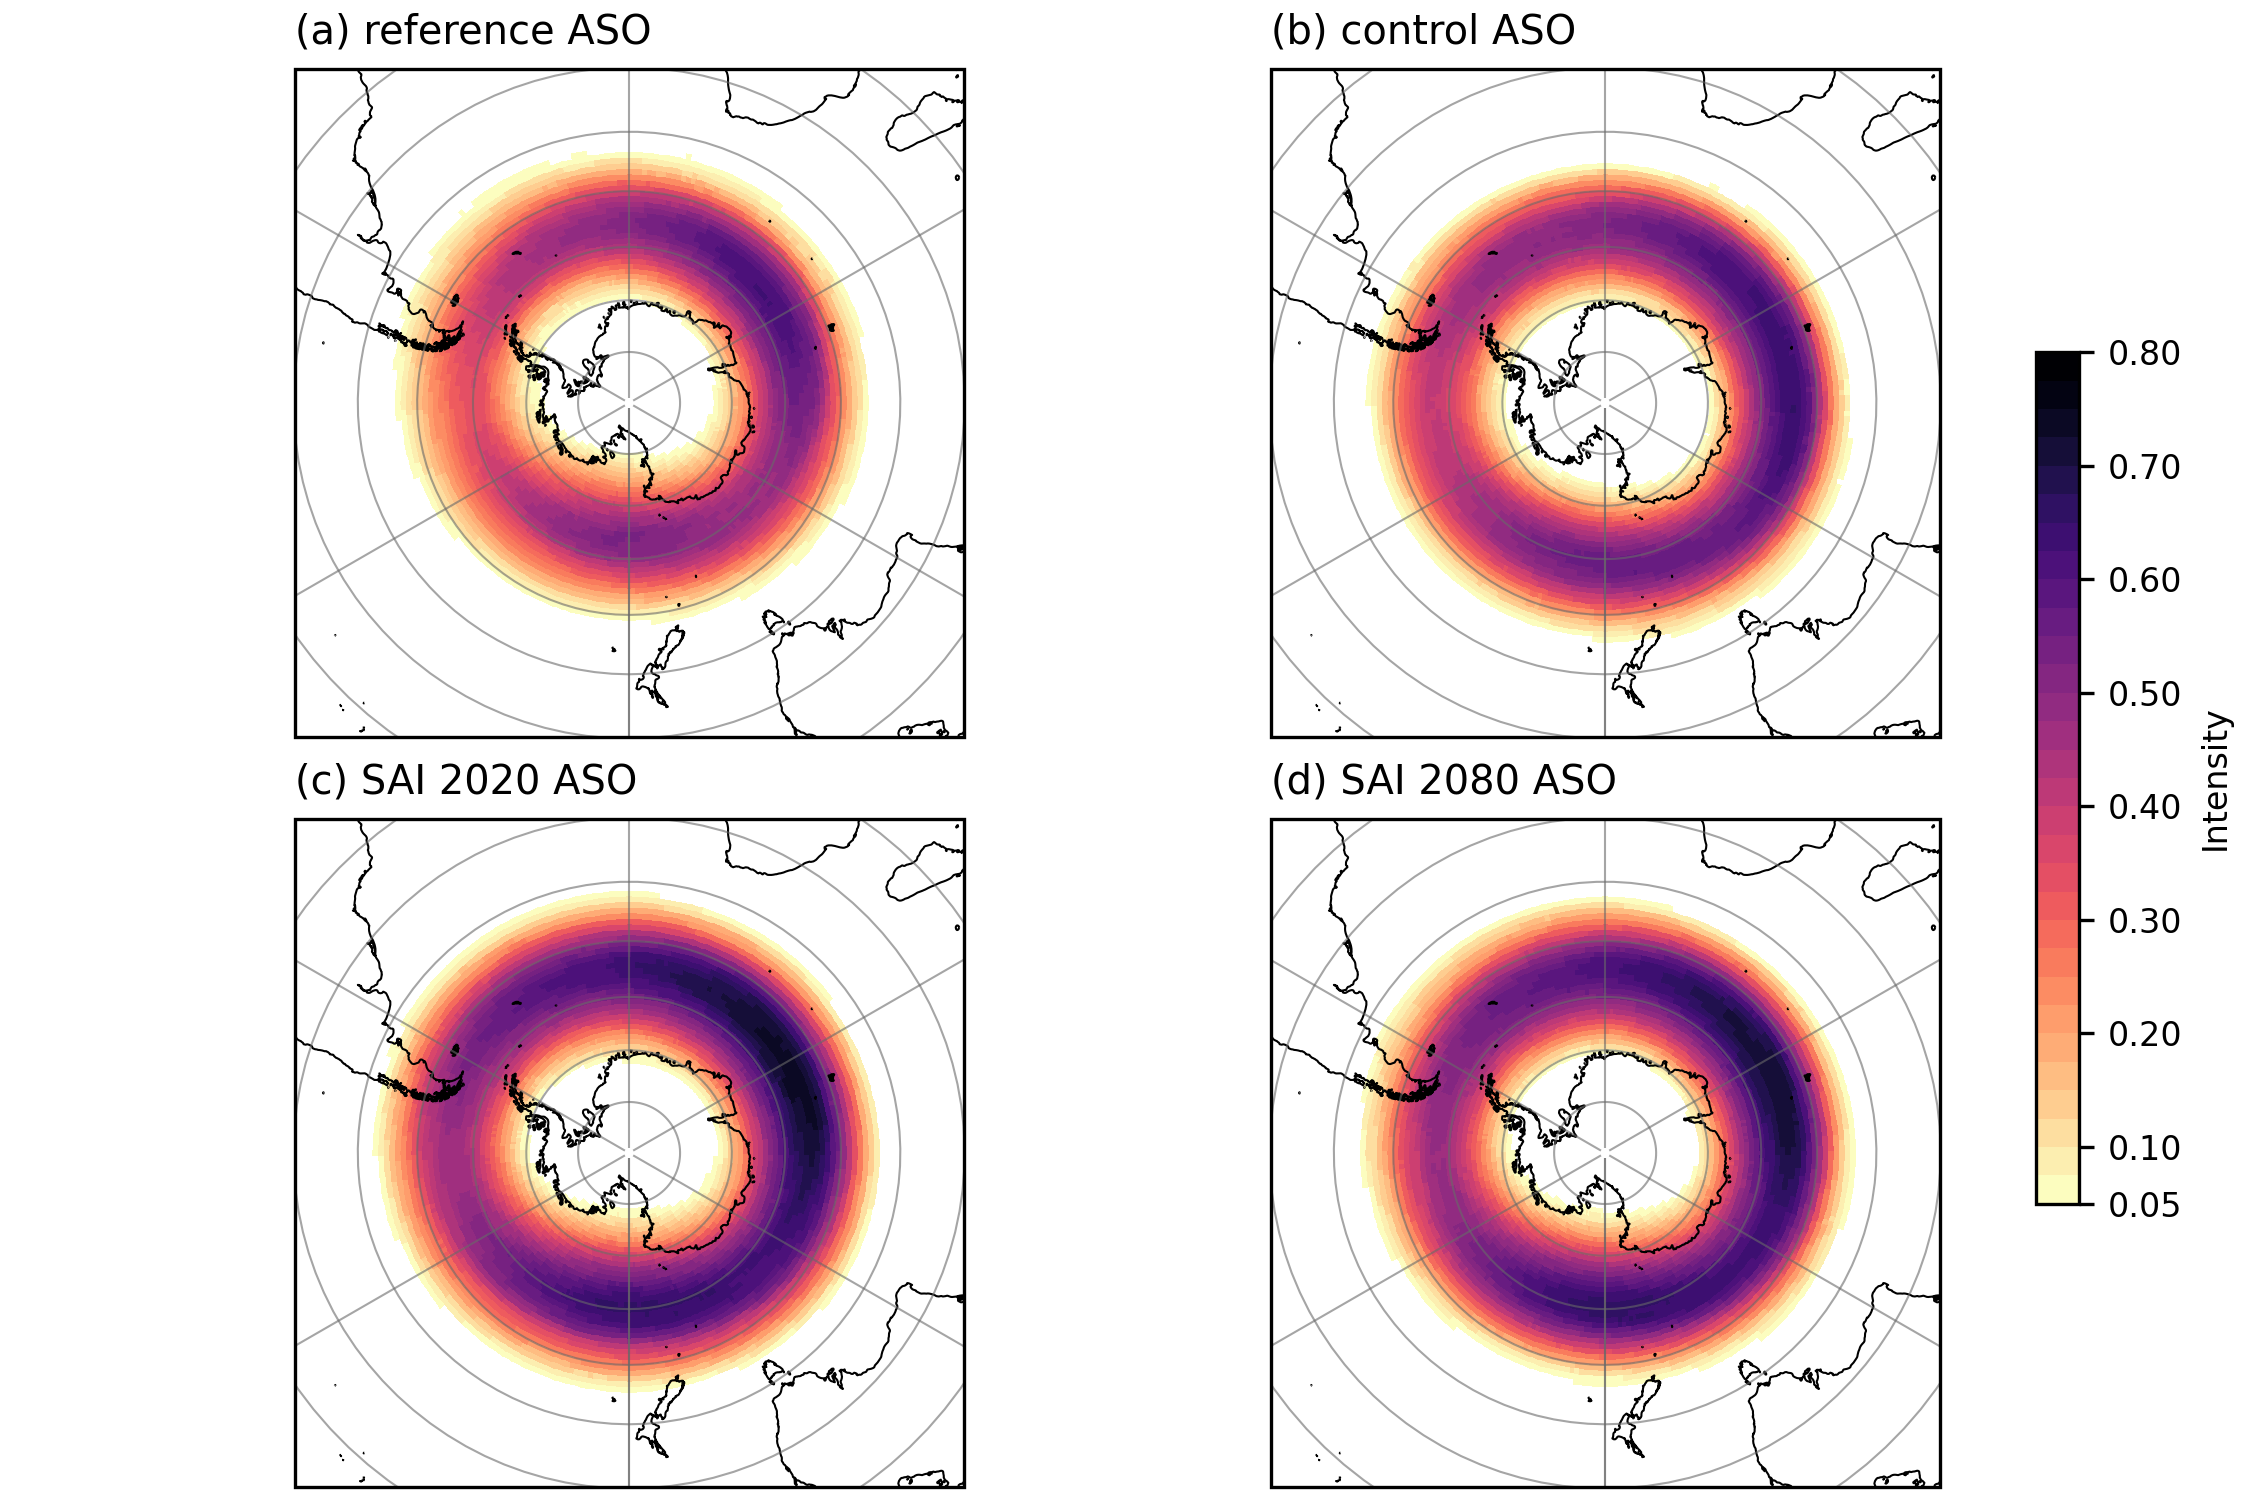
\includegraphics[width=0.95\linewidth]{images/PNJ_map.png}
	\caption{Polar night jet intensity map for (a) Reference, (b) Control, (c) SAI 2020 and (d) SAI 2080.}
	\label{fig:PNJ_map}
\end{figure}


\begin{figure}[H]
	\centering
	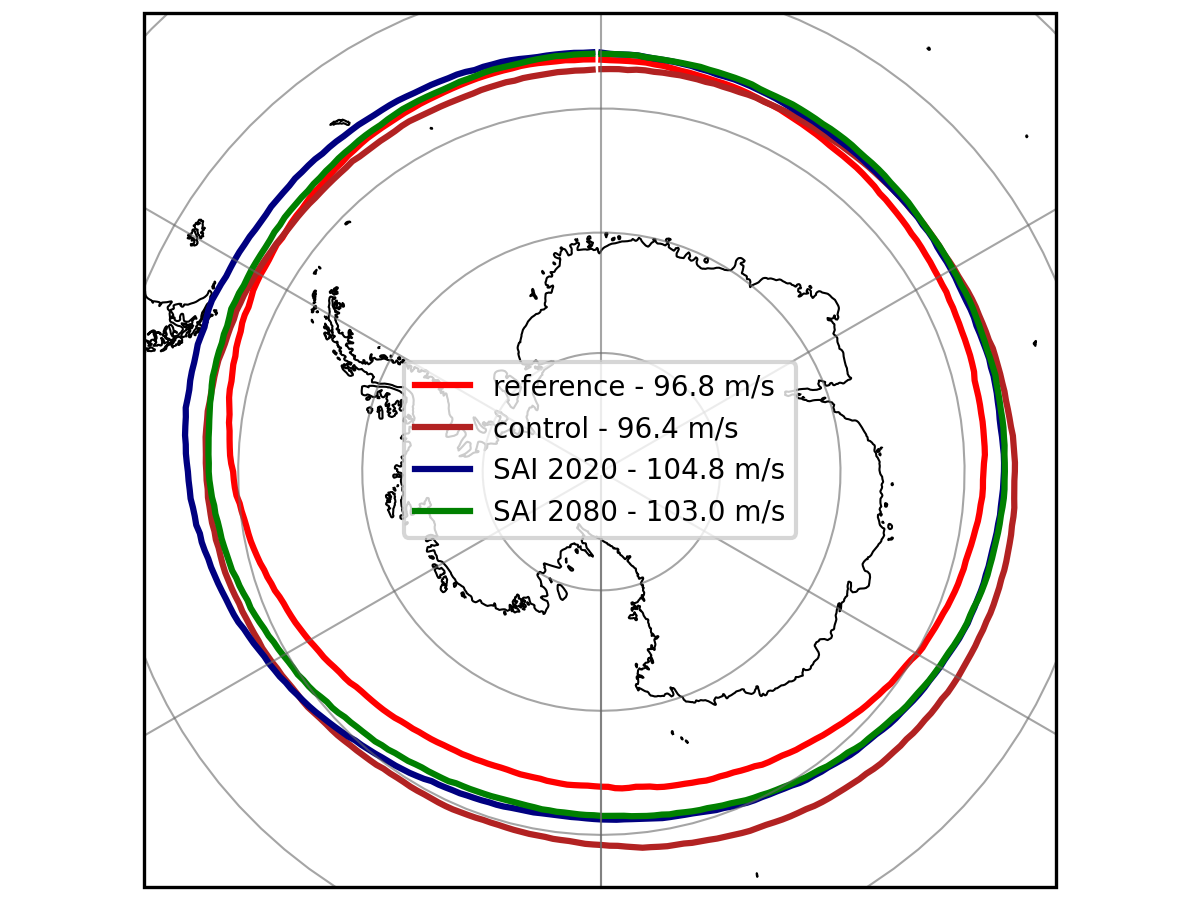
\includegraphics[width=0.48\linewidth]{images/PNJ_maxloc_latlon.png}
	\caption{Mean location of maximum wind speed at 10 hPa, with longitudinal mean maximum wind speed, for Reference, Control, SAI 2020 and SAI 2080.}
	\label{fig:PNJ_maxloc}
\end{figure}

\subsection{Sudden Stratospheric Warming Events}
The decrease in EKE over the Antarctic observed in \ref{fig:PNJ_EKE_U_zmdiff} suggests a decrease in the occurence of sudden stratospheric warming events (SSW). Figure \ref{fig:PNJ_climographTU} shows the area weighted mean temperature of the 10 hPa level above 60°S, together with the zonal wind at 10 hPa and 60°S. Note the  In Reference there is a number of years where the temperature increases and the zonal wind decreases compared to the mean. This indicates large scale SSW, as they are large enough, either in magnitude or duration, to show up in the monthly mean data. In Control the frequency of SSW-like conditions decreases significantly, the temperature and zonal wind bands narrow compared to Reference. In SAI 2020 there appears to be one year with SSW-like conditions, but again the temperature and zonal wind bands narrow. SAI 2080 shows the same trend. 

In all scenarios the zonal wind increases, as was already discussed in the results above, and the temperature decrease due to increased greenhouse gases is also visible. In all scenarios the PNJ forms earlier in the year, surpassing 75 m/s in early June in Control and late May in SAI 2020 and SAI 2080, as opposed to late June in Reference. The PNJ also dissolves later in the year, decreasing to 75 m/s in November in all scenarios as opposed to October in Reference.

\begin{figure}[H]
	\centering
	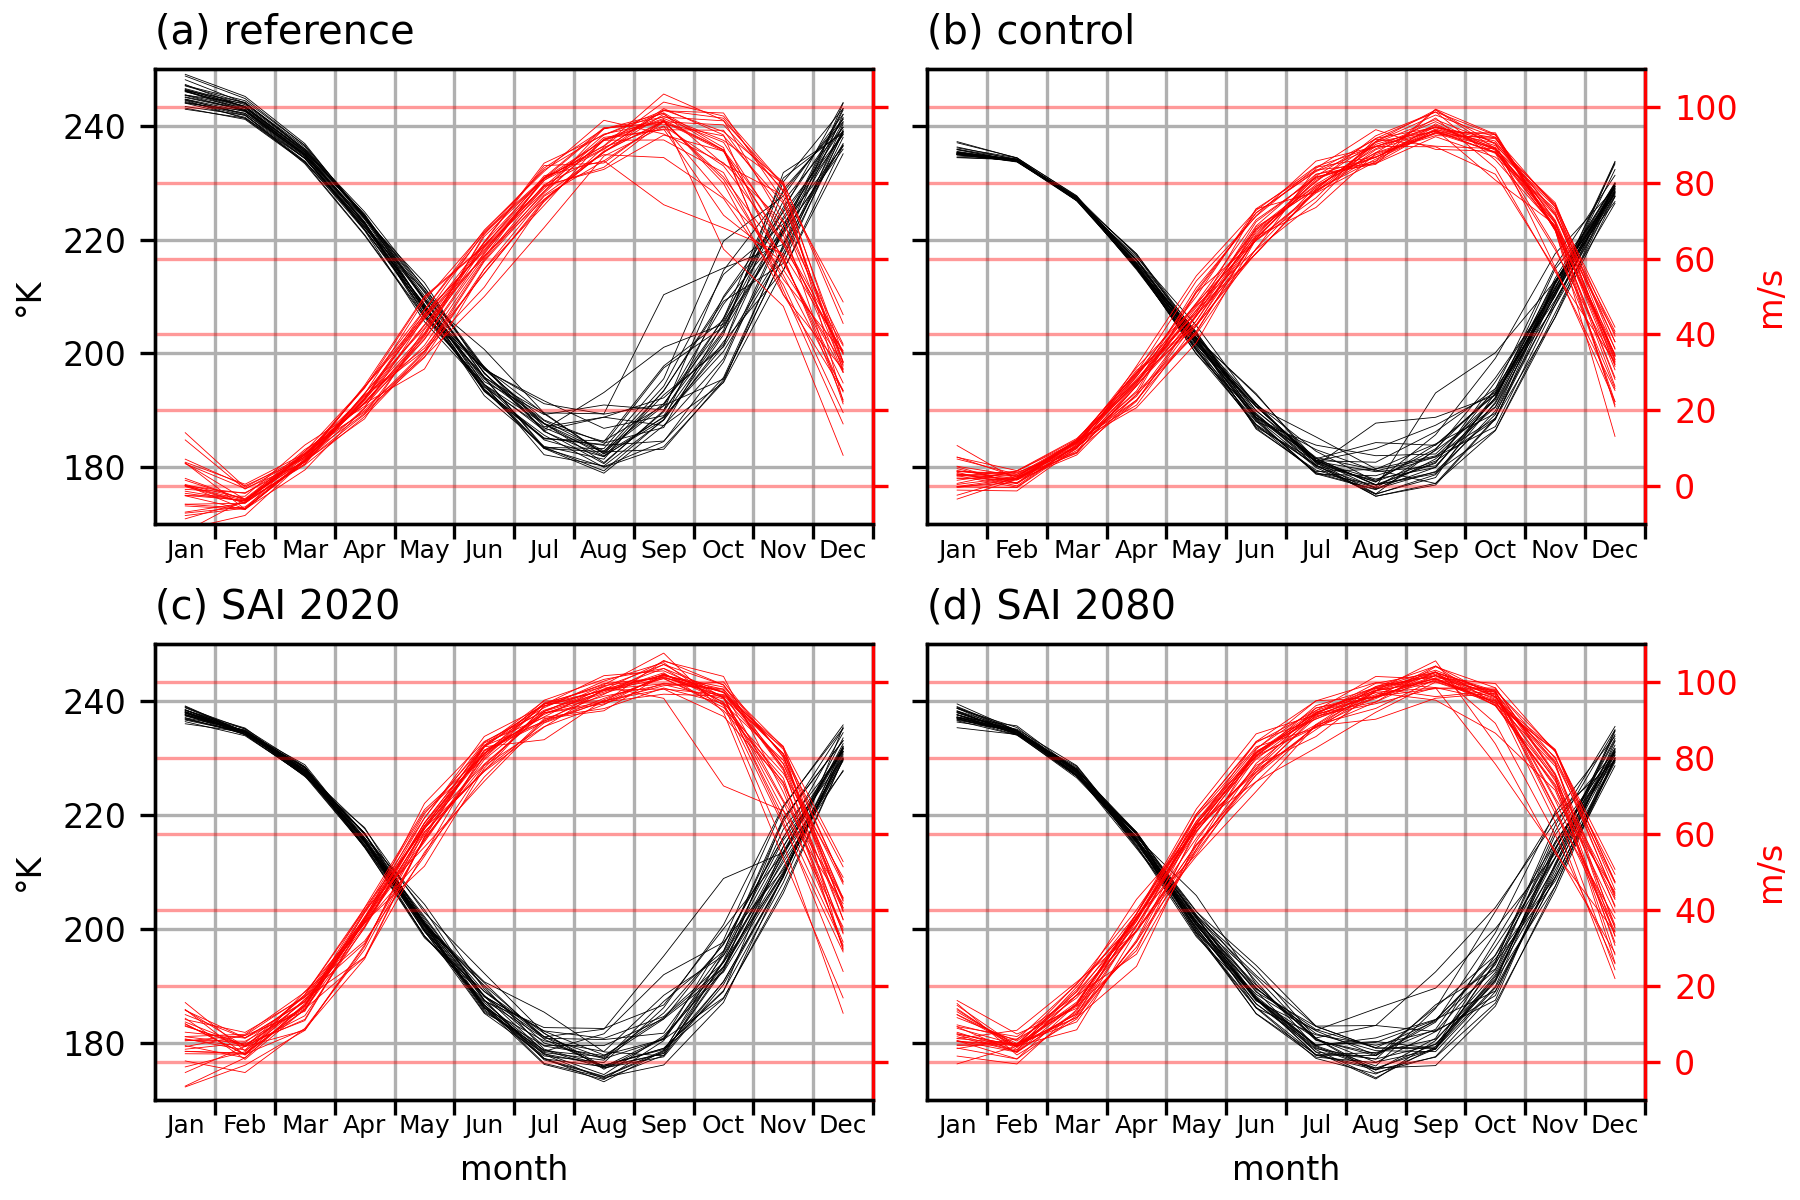
\includegraphics[width=0.95\linewidth]{images/PNJ_climographTU.png}
	\caption{Climograph of area-weighted mean temperature of 60°-90°S at 10 hPa (black) and zonal mean zonal wind at 60°S and 10 hPa (red) for (a) 2016-2045 and (b) 2101-2130 in the SSP5-8.5 experiment, (c) 2101-2130 in the gradual SAI experiment and (d) 2101-2130 in the rapid cooling SAI experiment.}
	\label{fig:PNJ_climographTU}
\end{figure}
\newpage 
\printbibliography

\end{document}
